\documentclass[11pt]{book}
\usepackage[slovene]{babel}
\usepackage[utf8]{inputenc}
\usepackage{amsmath}
\usepackage[dvipsnames]{xcolor}
\usepackage{titlesec}
% \usepackage{amssymb}
\usepackage{pstricks,pst-plot,pst-math}
\usepackage{pstricks-add}
\usepackage{graphicx}
\usepackage{enumerate}
\usepackage{color}
\usepackage{fouriernc}
\usepackage{microtype}
\usepackage{MnSymbol}
\usepackage{tikz-cd}
\usetikzlibrary{backgrounds}
\usepackage{wrapfig}
\usepackage{geometry}
\geometry{
    a4paper,
    left=45mm,
    right=45mm,
    top=20mm,
    bottom=20mm
    }
    \usepackage{comment}
    

\usepackage{amsthm}

\usepackage{changepage}   % for the adjustwidth environment
\usepackage{hyperref}
\hypersetup{
    colorlinks=true,
    linkcolor=cyan,
    filecolor=magenta,      
    urlcolor=cyan
    }

\usepackage[backgroundcolor=svetlosiva,linecolor=siva,textsize=footnotesize]{todonotes}

\pagestyle{plain}

\usepackage{enumitem}
\setlist[description]{leftmargin=\parindent,labelindent=\parindent, font=\normalfont\itshape\textbullet\space}


\def\NN{\mathbf{N}}
\def\ZZ{\mathbf{Z}}
\def\QQ{\mathbf{Q}}
\def\RR{\mathbf{R}}
\def\CC{\mathbf{C}}
\def\conclass{\mathcal{C}}
\def\11{\mathbf{1}}
\def\FF{\mathbf{F}}
\def\Fcal{\mathcal{F}}
\def\EE{\mathbf{E}}
\def\PP{\mathbf{P}}
\def\HH{\mathbf{H}}
\def\GG{\mathcal{G}}
\def\youngsym{\sigma_{\lambda}}

\DeclareMathOperator\image{im}
\DeclareMathOperator\sgn{sgn}
\DeclareMathOperator\Res{Res}
\DeclareMathOperator\Ind{Ind}
\DeclareMathOperator\Rep{Rep}
\DeclareMathOperator\mult{mult}
\DeclareMathOperator\Izotip{Izotip}
\DeclareMathOperator\MK{MK}
\DeclareMathOperator\tr{tr}
\DeclareMathOperator\Irr{Irr}
\DeclareMathOperator\SU{SU}
\DeclareMathOperator\characteristic{char}
\DeclareMathOperator\kk{k}
\DeclareMathOperator\cl{cl}
\def\GAP{\texttt{GAP}}
\DeclareMathOperator\inv{inv}
\DeclareMathOperator\Eigenvalues{Spec}
\DeclareMathOperator\Eigenspace{ES}
\DeclareMathOperator\fun{fun}
\DeclareMathOperator\HS{HS}
\DeclareMathOperator\St{St}
\DeclareMathOperator\Realpart{Re}

\DeclareMathOperator\DNO{DNO}
\DeclareMathOperator\KNO{KNO}


\DeclareMathOperator\Aut{Aut}
\DeclareMathOperator\GL{GL}
\DeclareMathOperator\glfrak{\mathfrak{gl}}
\DeclareMathOperator\slfrak{\mathfrak{sl}}
\DeclareMathOperator\U{U}
\DeclareMathOperator\SL{SL}
\DeclareMathOperator\PSL{PSL}
\DeclareMathOperator\SO{SO}
\DeclareMathOperator\Gal{Gal}
\DeclareMathOperator\Sym{Sym}
\DeclareMathOperator\Homeo{Homeo}
\DeclareMathOperator\Cay{Cay}
\DeclareMathOperator\Isom{Isom}
\DeclareMathOperator\id{id}
\DeclareMathOperator\supp{supp}
\DeclareMathOperator\End{End}
\DeclareMathOperator\Mat{Mat}
\DeclareMathOperator\Cone{Cone}
\DeclareMathOperator\diam{diam}
\DeclareMathOperator\Ad{Ad}
\DeclareMathOperator\imaginary{Im}

\def\definicija{\color{rdeca}\bf\em}
\def\vprasanje{\color{oranzna}}
\def\literatura{\color{modra}}
\def\vaje{{\literatura ($\to$ vaje)}}
\def\kljuka{$\checkmark$}

\theoremstyle{definition}

\newtheoremstyle{zgled}
 {}{}%
 {\color{zelena}}
 {}%
 {\color{zelena}\bfseries}%
 {\color{zelena}.}%
 { }{}

\theoremstyle{zgled}
\newtheorem*{zgled}{Zgled}

\newtheoremstyle{odprtproblem}
 {}{}%
 {\color{oranzna}}
 {}%
 {\color{oranzna}\bfseries}%
 {\color{oranzna}.}%
 { }{}

\theoremstyle{odprtproblem}
\newtheorem*{odprtproblem}{Odprt problem}

\newtheoremstyle{domacanaloga}
 {}{}%
 {\color{vijolicna}}
 {}%
 {\color{vijolicna}\bfseries}%
 {\color{vijolicna}.}%
 { }{}

\theoremstyle{domacanaloga}
\newtheorem*{domacanaloga}{Domača naloga}

\newenvironment{dokaz}
    {\color{siva}\begin{proof}}
    {\end{proof}}

\newtheoremstyle{izrek}
 {}{}% above, below 
 {\color{black}\itshape}
 {}% indent
 {\color{black}\bfseries}%
 {\color{black}.}%
 { }{}

\theoremstyle{izrek}
\newtheorem*{izrek}{Izrek}

\newtheorem*{trditev}{Trditev}
\newtheorem*{pomoznatrditev}{Pomožna trditev}

\newtheorem*{lema}{Lema}

\newtheorem*{posledica}{Posledica}

\newenvironment{povzetek}
    {
\smallskip
\begin{center}
\color{svetlosiva}
\begin{tabular}{|p{0.7\textwidth}}
    }
    {
\end{tabular}
\end{center}
\smallskip
    }


\definecolor{rdeca}{rgb}{0.62, 0.16, 0.10}
\definecolor{zelena}{rgb}{0.15, 0.4, 0.20}
\definecolor{oranzna}{rgb}{0.72, 0.38, 0.082}
\definecolor{rjava}{rgb}{0.7490196078431373, 0.3686274509803922, 0.1843137254901961}
\definecolor{modra}{rgb}{0.2784313725490196, 0.5411764705882353, 0.8392156862745098}
\definecolor{vijolicna}{rgb}{0.48627450980392156, 0.2980392156862745, 0.792156862745098}
\definecolor{siva}{rgb}{0.5, 0.5, 0.5}
\definecolor{svetlosiva}{rgb}{0.7, 0.7, 0.7}


\titleformat{\section}
  {\color{rdeca}\LARGE\bf}{\thesection}{1em}{}
\renewcommand{\thesubsection}{}
\titleformat{\subsection}
  {\Large\bf}{}{1em}{}

\title{\bf Diskretne stukture}
\author{Urban Jezernik}

% za generiranje html dokumenta s stilom mystyle.css uporabi:
% pandoc ds.tex --toc --toc-depth=2 --metadata date="`date -u "+%d. %m. %Y"`" --template template.html -c mystyle.css -s --mathjax -o index.html


\begin{document}

\baselineskip=14pt

\maketitle

\setcounter{tocdepth}{1}
\tableofcontents

\newpage

\subsection*{Kratek opis predmeta}

Pri predmetu se bomo najprej naučili, kaj točno so \emph{izjave} in kako jih matematično \emph{formalizirati}. Eden pomembnih ciljev tega je eksakten opis  \emph{sklepanja}, ki ga uporabljamo počez matematike. Te koncepte bomo najprej razvili v osnovnem \emph{izjavnem računu}, nato pa ga bomo še posplošili do \emph{predikatnega računa}, s katerim bomo podrobneje raziskali matematične izjave. 

\begin{zgled}
Nepridipravi so razbili vhodna vrata FMF. Glavni osumljenci so študenti Ana, Bor in Cveto. Ko jih vprašamo, kdo je kriv, odgovorijo z naslednjimi izjavami:

\begin{itemize}
    \item Ana: ``Bor je kriv, Cveto pa ne.''
    \item Bor: ``Če je kriva Ana, je kriv tudi Cveto.''
    \item Cveto: ``Jaz nisem kriv, toda vsaj eden od drugih dveh je kriv.''
\end{itemize}

Pri predmetu se bomo naučili, kako lahko na \emph{sistematičen način} odkrijemo, kdo je lagal, če krivi lažejo, nedolžni pa govorijo resnico.
\end{zgled}

Za tem bomo pri predmetu spoznali nekaj osnovnih diskretnih struktur, po katerih se ta predmet imenuje. Najprej bomo raziskali \emph{relacije}, s katerimi opisujemo odnose med elementi dane množice. Pomemben poseben primer teh so \emph{urejenosti}, ki posplošujejo običajne ureditve števil po velikosti. Najbolj podrobno si bomo ogledali \emph{grafe}, s katerimi lahko abstraktno predstavimo mnogo pomembnih primerov relacij.

\begin{zgled}
Graf je diskretna struktura, pri kateri dano množico \emph{vozlišč} povežemo s \emph{povezavami}. Z grafi lahko opišemo veliko različnih vrst omrežij, na primer internetno omrežje, omrežje prijateljskih povezav na Facebooku, omrežja veriženja blokov (kriptovalute) \dots 

Konkreten graf na spodnji sliki se imenuje {\definicija Petersenov graf}. Ta graf bomo tekom predmeta večkrat srečali. Na koncu predmeta bomo znali \emph{dokazati}, da se tega grafa ne da narisati v ravnini, brez da bi se vsaj dve povezavi sekali.

\begin{figure}[h]
    \centering
    \includegraphics[width=0.5\linewidth]{img/opis-petersen.png}
    \caption{Petersenov graf}
\end{figure}
\end{zgled}

\newpage

\subsection*{Literatura}

\begin{itemize}
\item {\literatura G. Fijavž, \href{http://matematika.fri.uni-lj.si/ds/ds.pdf}{\emph{Diskretne strukture}}, elektronska knjiga, 2015.} 
\item {\literatura M. Juvan in P. Potočnik, \href{http://www.dmfa-zaloznistvo.si/ipmr/1662.htm}{\emph{Teorija grafov in kombinatorika}}, DMFA-založništvo, Ljubljana 2000.}
\item {\literatura N. Prijatelj, \emph{Osnove matematične logike I}, DMFA-založništvo, Ljubljana, 1992.}
\end{itemize}

\todo{Dodaj literaturo za vaje.}

\chapter{Izjavni račun}

V tem poglavju si bomo pogledali, kako \emph{formaliziramo} preproste izjave in kako \emph{dokazujemo} njihovo veljavnost oziroma neveljavnost.

\section{Izjave in izjavni vezniki}

{\definicija Izjava} je poved, ki je bodisi resnična bodisi lažna.

\begin{zgled} \leavevmode
\begin{itemize}
    \item Ena in ena je tri. \emph{Lažna izjava.}
    \item Ena in ena je dve. \emph{Resnična izjava.}
    \item Koliko je ena in ena? \emph{Ni izjava.}
    \item Pojdimo na kavo! \emph{Ni izjava.}
\end{itemize}
\end{zgled}

Izjave lahko razdelimo na dve skupini \emph{po vsebini}, in sicer:
\begin{itemize}
    \item {\definicija resnične izjave}, ki imajo resničnostno vrednost $1$ ali $\top$ ali \texttt{true},
    \item {\definicija lažne izjave}, ki imajo resničnostno vrednost $0$ ali $\bot$ ali \texttt{false}.
\end{itemize}
Po \emph{zgradbi} oziroma \emph{obliki} pa izjave razdelimo na:
\begin{itemize}
    \item {\definicija osnovne}, ki ne vsebujejo izjavnih veznikov,
    \item {\definicija sestavljene}, ki vsebujejo izjavne veznike.
\end{itemize}

\begin{zgled} \leavevmode
\begin{itemize}
    \item Vreme je lepo. \emph{Osnovna izjava.}
    \item Špela gre v hribe. \emph{Osnovna izjava.}
    \item Vreme je lepo \emph{in} Špela gre v hribe. \emph{Sestavljena izjava.}
    \item \emph{Če} je vreme lepo, \emph{potem} gre Špela v hribe. \emph{Sestavljena izjava.}
    \item Špela \emph{ne} gre v hribe. \emph{Sestavljena izjava.}
\end{itemize}
\end{zgled}

Naj bo $n \in \NN_0$. {\definicija Izjavni veznik reda $n$} (ali {\definicija $n$-mestni izjavni veznik}) je funkcija, ki vsaki urejeni $n$-terici ničel in enic priredi vrednost $0$ ali $1$.

\begin{zgled} \leavevmode
\begin{itemize}
    \item Primer izjavnega veznika reda $1$ je {\definicija negacija}. Simbol za ta veznik je $\lnot$. Če je $p$ izjava, njeno negacijo označimo kot $\lnot p$ in preberemo kot \emph{ne $p$} ali kot \emph{ni res, da velja $p$}. Negacija $1$-terici $0$ priredi vrednost $1$, $1$-terici $1$ pa priredi vrednost $0$.
    
    \begin{table}[h]
        \centering
        \begin{tabular}{c|c}
            $p$ & $\lnot p$ \\ \hline
            0 & 1 \\
            1 & 0
        \end{tabular}
        \caption{Resničnostna tabela negacije}
    \end{table}

    \item Oglejmo si nekaj pomembnih dvomestnih izjavnih veznikov. Njihovi predpisi so zbrani v tabeli.
    \begin{itemize}
        \item {\definicija Konjunkcija} izjav $p$ in $q$ ima simbol $p \land q$, kar preberemo kot \emph{$p$ in $q$}.
        \item {\definicija Disjunkcija} izjav $p$ in $q$ ima simbol $p \lor q$, kar preberemo kot \emph{$p$ ali $q$}.
        \item {\definicija Implikacija} izjav $p$ in $q$ ima simbol $p \Rightarrow q$, kar preberemo kot \emph{če $p$, potem $q$} ali kot \emph{iz $p$ sledi $q$} ali kot \emph{$p$ je zadosten pogoj za $q$} ali \emph{kot $q$ je potreben pogoj za $p$}.
        \item {\definicija Ekvivalenca} izjav $p$ in $q$ ima simbol $p \Leftrightarrow q$, kar preberemo kot \emph{$p$ natanko tedaj, ko $q$} ali kot \emph{$p$, če in samo če $q$} ali kot \emph{$p$ je ekvivalentno $q$}.
    \end{itemize}

    \begin{table}[h]
        \centering
        \begin{tabular}{cc|cccc}
            $p$ & $q$ & $p \land q$ & $p \lor q$ & $p \Rightarrow q$ & $p \Leftrightarrow q$ \\ \hline
            1 & 1 & 1 & 1 & 1 & 1 \\
            1 & 0 & 0 & 1 & 0 & 0 \\
            0 & 1 & 0 & 1 & 1 & 0 \\
            0 & 0 & 0 & 0 & 1 & 1
        \end{tabular}
        \caption{Resničnostna tabela nekaterih pomembnih dvomestnih izjavnih veznikov}
    \end{table}

    \item Izjavni veznik reda $0$ je funkcija iz množice urejenih $0$-teric ničel in enic. Obstaja natanko ena taka $0$-terica, in sicer \emph{prazna $0$-terica}. Izjavni veznik reda $0$ je torej natanko določen s sliko te $0$-terice, za kar imamo dve možnosti, $0$ ali $1$.
    \begin{itemize}
        \item Izjavni veznik reda $0$, ki ima vselej resničnostno vrednost $0$, imenujemo {\definicija 0} in preberemo kot \emph{lažna izjava}.
        \item Izjavni veznik reda $0$, ki ima vselej resničnostno vrednost $1$, imenujemo {\definicija 1} in preberemo kot \emph{resnična izjava}.
    \end{itemize}
    Izjavnima veznikoma reda $0$ pravimo tudi {\definicija izjavni konstanti}.
\end{itemize}
\end{zgled}

Glede na zgornjo obravnavamo izjavnih veznikov redov $0$, $1$ in $2$ se lahko vprašamo, koliko je vseh $n$-mestnih izjavnih veznikov za poljuben $n \in \NN_0$. Vsak tak veznik je enolično določen s svojo resničnostno tabelo, v kateri zabeležimo vrednosti veznika v {\definicija izjavnih spremenljivkah} $p_1, p_2, \dots, p_n$, kjer vsak $p_i$ zavzema vrednosti $0$ ali $1$.

\begin{table}[h]
    \centering
    \begin{tabular}{cccc|c}
        $p_1$ & $p_1$ & $\cdots$ & $p_n$ & veznik($p_1$, $p_2$, \dots, $p_n$) \\ \hline
        1 & 1 & $\cdots$ & 1 & 0 ali 1 \emph{(dve možnosti)} \\
        1 & 1 & $\cdots$ & 0 & 0 ali 1 \emph{(dve možnosti)} \\
        $\vdots$ & $\vdots$ & & $\vdots$ & $\vdots$ \\
        0 & 0 & $\cdots$ & 0 & 0 ali 1 \emph{(dve možnosti)} \\
    \end{tabular}
    \caption{Resničnostna tabela $n$-mestnega izjavnega veznika}
\end{table}

Število vseh $n$-mestnih izjavnih veznikov torej izračunamo tako, da preštejemo število vseh možnih resničnostnih tabel. Število vrstic tabele je enako $2^n$, število vseh tabel pa je zato enako $2^{2^n}$.

\begin{table}[h]
    \centering
    \begin{tabular}{c|cc}
        $n$ & $2^n$ & $2^{2^n}$ \\ \hline
        0 & 1 & 2 \\
        1 & 2 & 4 \\
        2 & 4 & 16 \\
        3 & 8 & 256 \\
        4 & 16 & 65536 \\
        5 & 32 & $\sim 4 \cdot 10^9$ \\
        6 & 64 & $\sim 2 \cdot 10^{19}$
    \end{tabular}
    \caption{Hitra rast števila $n$-mestnih izjavnih veznikov}
\end{table}

\section{Izjavni izrazi}

{\definicija Izjavni izraz} definiramo induktivno na naslednji način:
\begin{itemize}
    \item \emph{Osnovni izraz 1:} Vsaka \emph{izjavna konstanta} (torej $0$ ali $1$) je izjavni izraz. 
    \item \emph{Osnovni izraz 2:} Vsaka \emph{izjavna spremenljivka} $p_1, p_2, \dots$ je izjavni izraz.
    \item \emph{Sestavljeni izraz:} Če je $f$ \emph{izjavni veznik} reda $n$ in so $A_1, A_2, \dots, A_n$ izjavni izrazi, potem je $(f(A_1,A_2,\dots,A_n))$ izjavni izraz.
\end{itemize}

Izjavni izrazi so torej izjave, ki jih dobimo iz $0,1$ in izjavnih spremenljivk z (večkratno) uporabo izjavnih veznikov.

\begin{zgled}
    Naj bodo $p,q,r$ izjavne spremenljivke. Tvorimo lahko izjavne izraze $(p \Rightarrow q)$, $(\lnot r)$, $((p \Rightarrow q) \land (\lnot r))$, \dots
\end{zgled}

Pri pisanju bolj zakompliciranih izjavnih izrazov se prične pojavljati mnogo oklepajev. V izogib pisanju prevelikega števila teh oklepajev uporabljamo naslednji {\definicija dogovor o prednostnem vrstnem redu veznikov}:
\begin{itemize}
    \item $\lnot$ ima prednost pred dvomestnimi vezniki,
    \item veznik iz $(\land, \lor, \Rightarrow, \Leftrightarrow)$ ima prednost pred vezniki desno od sebe,
    \item če isti veznik nastopi večkrat zapored, ima levi nastop prednost pred desnim,
    \item zunanji oklepaj spuščamo.
\end{itemize}

\begin{zgled} \leavevmode
\begin{itemize}
    \item Izjavni izraz $(p \Rightarrow (q \land r))$ pišemo krajše kot $p \Rightarrow q \land r$.
    \item Izraz $p \Rightarrow q \Rightarrow r \Rightarrow s$ je okrajšava za izjavni izraz $(((p \Rightarrow q) \Rightarrow r) \Rightarrow s)$.
    \item Izraz $p \lor \lnot q \Leftrightarrow r \Rightarrow q$ je okrajšava za izjavni izraz $(( p \lor (\lnot q)) \Leftrightarrow (r \Rightarrow p))$.
\end{itemize}
\end{zgled}

Izjavni izrazi vsebujejo izjavne spremenljivke, zato določajo neko resničnostno tabelo in s tem tudi nek izjavni veznik.

\begin{zgled}
Naj bodo $p,q,r$ izjavne spremenljivke in naj bo $f(p,q,r) = (p \Rightarrow q) \land \lnot r$ izjavni izraz. Izračunamo lahko resničnostno tabelo tega izraza in na ta način lahko na $f$ gledamo kot na izjavni veznik reda $3$.

\begin{table}[h]
    \centering
    \begin{tabular}{ccc|c}
        $p$ & $q$ & $r$ & $(p \Rightarrow q) \land \lnot r$ \\ \hline
        1 & 1 & 1 & 0 \\
        1 & 1 & 0 & 1 \\
        1 & 0 & 1 & 0 \\
        1 & 0 & 0 & 0 \\
        0 & 1 & 1 & 0 \\
        0 & 1 & 0 & 1 \\
        0 & 0 & 1 & 0 \\
        0 & 0 & 0 & 1
    \end{tabular}
    \caption{Resničnostna tabela izjavnega izraza $(p \Rightarrow q) \land \lnot r$}
\end{table}
\end{zgled}

\section{Tavtologije in enakovredni izrazi}

Če je izjavni izraz \emph{resničen} pri vseh naborih svojih izjavnih spremenljivk, mu rečemo {\definicija tavtologija}. Če je \emph{lažen} pri vseh naborih, mu rečemo {\definicija protislovje}. Če ni niti tavtologija niti protislovje, je {\definicija kontingenten}.

\begin{zgled} \leavevmode
\begin{itemize}
    \item Izjavna izraza $1$ in $p \lor \lnot p$ sta tavtologiji.
    \item Izjavna izraza $0$, $p \land \lnot p$ sta protislovji.
    \item Izračunajmo resničnostne tabele izjavnih izrazov $p \Rightarrow q \Leftrightarrow \lnot p \lor q$, $p \land \lnot (q \Rightarrow p)$ in $p \land (\lnot q \lor p)$. 
    
    \begin{table}[h]
        \centering
        \begin{tabular}{cc|ccc}
            $p$ & $q$ & $p \Rightarrow q \Leftrightarrow \lnot p \lor q$ & $p \land \lnot (q \Rightarrow p)$ & $p \land (\lnot q \lor p)$ \\ \hline
            1 & 1 & 1 & 0 & 1 \\
            1 & 0 & 1 & 0 & 1 \\
            0 & 1 & 1 & 0 & 0 \\
            0 & 0 & 1 & 0 & 0 \\
        \end{tabular}
        \caption{Resničnostne tabele treh izjavnih izrazov}
    \end{table}

    Vidimo, da je prvi izraz tavtologija, drugi protislovje, tretji pa kontingenten.

    \begin{domacanaloga}
        Prepričaj se, da je resničnostna tabela izjavnega izraza $p \land (\lnot q \lor p)$ enaka resničnosti tabeli izjavnega izraza $p$. Sklepaj, da je izjava $p \land (\lnot q \lor p) \Leftrightarrow p$ tavtologija. Na podoben način se prepričaj, da je izraz $p \Rightarrow q \Leftrightarrow \lnot q \Rightarrow \lnot p$ tavtologija.
    \end{domacanaloga}        
\end{itemize}
\end{zgled}

Naj bosta $A$ in $B$ izjavna izraza. Kadar je $A \Leftrightarrow B$ tavtologija, tedaj rečemo, da sta izraza $A$ in $B$ {\definicija enakovredna}. Z drugimi besedami, izraza $A$ in $B$ sta enakovrednosta, kadar imata enaka stolpca v resničnostni tabeli. V tem primeru uporabimo oznako $A \sim B$.

\begin{zgled}
Velja $p \Rightarrow q \sim \lnot p \lor q \sim \lnot q \Rightarrow \lnot p$ in $p \land (\lnot q \lor p) \sim p$.
\end{zgled}

Enakovrednemu paru izjavnih izrazov $A \sim B$ rečemo {\definicija zakoni izjavnega računa}. V vsakem izjavnem izrazu lahko poljuben izraz zamenjamo z enakovrednim in s tem poenostavimo izjavni izraz.

\begin{zgled}
Velja
\[
    p \land (\lnot q \lor p) \Rightarrow (\lnot q \Rightarrow \lnot p) \sim
    p \Rightarrow (p \Rightarrow q).
\]
\end{zgled}

Navedimo nekaj uporabnih zakonov izjavnega računa, ki veljajo za vse izjavne izraze $A,B,C$.
\begin{itemize}
    \item $\lnot 0 \sim 1$, $\lnot 1 \sim 0$
    \item $A \land 0 \sim 0$, $A \land 1 \sim A$, $A \lor 0 \sim A$, $A \lor 1 \sim 1$
    \item $A \land A \sim A$, $A \lor A \sim A$ ({\definicija idempotentnost})
    \item $A \land B \sim B \land A$, $A \lor B \sim B \lor A$ ({\definicija komutativnost})
    \item $A \land (B \land C) \sim (A \land B) \land C$, $A \lor (B \lor C) \sim (A \lor B) \lor C$ ({\definicija asociativnost})
    \item $A \land (A \lor B) \sim A$, $A \lor (A \land B) \sim A$ ({\definicija absorpcija})
    \item $A \land (B \lor C) \sim (A \land B) \lor (A \land C)$, $A \lor (B \land C) \sim (A \lor B) \land (A \lor C)$ ({\definicija distributivnost})
    \item $\lnot \lnot A \sim A$ ({\definicija dvojna negacija})
    \item $\lnot (A \land B) \sim \lnot A \lor \lnot B$, $\lnot (A \lor B) \sim \lnot A \land \lnot B$ ({\definicija De Morganova zakona})
    \item $A \Rightarrow B \sim \lnot B \Rightarrow \lnot A$ ({\definicija kontrapozicija}), $A \Rightarrow B \sim \lnot A \lor B$
    \item $A \Leftrightarrow B \sim (A \Rightarrow B) \land (B \Rightarrow A)$
\end{itemize}

\begin{zgled}
Izjavni izraz iz zadnjega zgleda lahko z naštetimi zakoni poenostavimo do
\[
    p \Rightarrow (p \Rightarrow q) \sim
    \lnot p \lor (\lnot p \lor q) \sim
    (\lnot p \lor \lnot p) \lor q \sim
    \lnot p \lor q \sim
    p \Rightarrow q.
\]
\end{zgled}

\section{DNO in KNO}

Do sedaj smo govorili o tem, kako za dan izjavni izraz določimo njegovo resničnostno tabelo. V tem razdelku si bomo zastavili obratno nalogo. Recimo, da je dana resničnostna tabela nekega kontingentnega izjavnega izraza $A$. Pokazali bomo, da lahko zgolj z uporabo izjavnih veznikov $\lnot$, $\land$, $\lor$ sestavimo izjavni izraz $D$, tako da bo $A \sim D$. Za začetek si oglejmo, kako to naredimo na enem konkretnem primeru.

\begin{zgled}
Naj bo izjavni izraz $A$ dan z resničnostno tabelo $T$.

\begin{table}[h]
    \centering
    \begin{tabular}{ccc|c}
        $p$ & $q$ & $r$ & $A$ \\ \hline
        1 & 1 & 1 & 0 \\
        1 & 1 & 0 & 1 \\
        1 & 0 & 1 & 0 \\
        1 & 0 & 0 & 0 \\
        0 & 1 & 1 & 0 \\
        0 & 1 & 0 & 1 \\
        0 & 0 & 1 & 0 \\
        0 & 0 & 0 & 1
    \end{tabular}
    \caption{Resničnostna tabela $T$ izjavnega izraza $A$}
\end{table}

Iskani izjavni izraz $D$ mora biti resničen natanko v 2., 6. in 8. vrstici tabele $T$. To je res natanko tedaj, ko velja $p \land q \land \lnot r$ ali $\lnot p \land q \land \lnot r$ ali $\lnot p \land \lnot q \land \lnot r$. Torej lahko vzamemo preprosto
\[
    D = (p \land q \land \lnot r) \lor (\lnot p \land q \land \lnot r) \lor (\lnot p \land \lnot q \land \lnot r)
\]
in res velja $D \sim A$. Dobljeni izjavni izraz $D$ lahko še nekoliko poenostavimo. 

\begin{domacanaloga}
    Z uporabo zakonov izjavnega računa se prepričaj, da velja $D \sim \lnot (p \Rightarrow q \Rightarrow r)$.
\end{domacanaloga}
\end{zgled}

Naj bo zdaj $A$ poljuben kontingenten izjavni izraz in $T$ njegova resničnostna tabela. {\definicija Disjunktivna normalna oblika} izraza $A$ je disjunkcija \emph{osnovnih konjunkcij} tistih vrstic, kjer je $A$ resničen. Pri tem je osnovna konjunkcija neke vrstice konjunkcija tistih izjavnih spremenljivk, ki so v tej vrstici resnične, in negacij tistih izjavnih spremenljivk, ki so v tej vrstici lažne. Disjunktivno normalno obliko izraza $A$ krajše pišemo kot $\DNO(A)$.

\begin{zgled}
V zadnjem zgledu je $\DNO(A) = D$.
\end{zgled}

Disjunktivna normalna oblika $\DNO(A)$ je izjavni izraz, ki je zapisan le z uporabo izjavnih veznikov $\lnot$, $\land$, $\lor$. Preverimo še, da je ta izraz res enakovreden začetnemu izrazu $A$.

\begin{trditev}
Naj bo $A$ kontingenten izraz. Potem je $A \sim \DNO(A)$.
\end{trditev}
\begin{dokaz}
Naj bo $T$ resničnostna tabela izraza $A$. Naj bo $i$ poljubna vrstica $T$. Dokazati želimo, da imata $T$ in $\DNO(A)$ v tej vrstici enako resničnostno vrednost.

\begin{description}
    \item[Če je $A$ resničen v vrstici $i$:] Po definiciji disjunktivne normalne oblike je $\DNO(A)$ disjunkcija osnovnih konjunkcij vrstic $T$. V posebnem osnovna konjunkcija vrstice $i$ nastopa v $\DNO(A)$. Ta osnovna konjunkcija je v vrstici $i$ resnična, zato je resnična tudi disjunkcija $\DNO(A)$. \kljuka
    \item[Če je $\DNO(A)$ resničen v vrstici $i$:] V tem primeru mora biti resničen vsaj en člen disjunkcije $\DNO(A)$, torej mora biti v vrstici $i$ resnična osnovna konjunkcija neke vrstice $j$. Osnovna konjunkcija vrstice $j$ je izraz, ki je v vrstici $j$ resničen, v vseh ostalih vrsticah pa lažen. Od tod sledi, da je $i = j$. Torej $\DNO(A)$ vsebuje osnovno konjunkcijo vrstice $i$, zato je $A$ resničen v vrstici $i$. \kljuka
\end{description}

Res imata torej $T$ in $\DNO(A)$ enake resničnostne vrednosti, torej sta $A$ in $\DNO(A)$ enakovredna.
\end{dokaz}

V sestavljanju disjunktivne normalne oblike smo opazovali vrstice, kjer je dan izjavni izraz $A$ resničen. Analogno bi lahko opazovali vrstice, kjer je izraz $A$ lažen, in sestavili izjavni izraz, ki bo \emph{lažen} natanko v vrsticah, v katerih je $A$ lažen. Na primeru pojasnimo, kako lahko na ta način dobimo alternativen izjavni izraz, ki je zopet izražen le z vezniki $\lnot$, $\land$, $\lor$ in je enakovreden izrazu $A$.

\begin{zgled}
Naj bo $T$ resničnostna tabela izjavnega izraza $A$ iz predzadnjega zgleda. Ta tabela je lažna v vrsticah $1,3,4,5,7$. Sestavimo izjavni izraz $K$, ki bo lažen natanko v teh vrsticah. To je enakovredno zahtevi, da je $K$ resničen natanko tedaj, ko nismo v nobeni od vrstic $1,3,4,5,7$. Slednjo zahtevo lahko izrazimo kot konjunkcijo \emph{osnovnih  disjunkcij} vrstic $1,3,4,5,7$, se pravi kot
\[
    K = 
    (\lnot p \lor \lnot q \lor \lnot r) \land
    (\lnot p \lor q \lor \lnot r) \land
    (\lnot p \lor q \lor r) \land
    (o \lor \lnot q \lor \lnot r) \land
    (p \lor q \lor \lnot r).
\]
Tako sestavljenemu izravnemu izrazu $K$ pravimo {\definicija konjunktivna normalna oblika} izraza $A$, krajše $\KNO(A)$. Sorodno kot za disjunktivno normalno obliko se prepričamo, da velja $\KNO(A) \sim A$.
\end{zgled}

\section{Sklepanje v izjavnem računu}

{\definicija Sklep} je končno zaporedje izjav $p_1, p_2, \dots, p_k, z$. Pri tem izjavam $p_1, p_2, \dots, p_k$ pravimo {\definicija predpostavke}, izjavi $z$ pa {\definicija zaključek}.

\begin{zgled}
Opazujmo naslednje zaporedje izjav.

\begin{description}
    \item[$p_1$:] Če je ta žival ptič, potem ima krila.
    \item[$p_2$:] Ta žival nima kril.
    \item[$z$:] Ta žival ni ptič. 
\end{description}

Imamo torej sklep $p_1, p_2, z$. Ta sklep lahko zapišemo nekoliko bolj natančno z upoštevanjem sestavljene strukture izjav v sklepu. Uvedimo izjavi $p$ in $q$ kot:

\begin{description}
    \item[$p$:] Ta žival je ptič.
    \item[$q$:] Ta žival ima krila.  
\end{description}

Sklep $p_1, p_2, z$ lahko torej zapišemo v obliki $p \Rightarrow q, \ \lnot q, \ \lnot p$.
\end{zgled}

Zaporedje izjavnih izrazov $A_1, A_2, \dots, A_k, B$ je {\definicija pravilen sklep} (rekli bomo tudi {\definicija veljaven sklep}), če je zaključek $B$ resničen pri vseh tistih naborih izjavnih spremenljivk, pri katerih so resnične vse predpostavke $A_1, A_2, \dots, A_k$. V tem primeru pišemo $A_1, A_2, \dots, A_k \models B$.

\begin{zgled}
Sklep iz zadnjega zgleda smo zapisali v obliki $p \Rightarrow q, \ \lnot q, \ \lnot p$. Če pri tem gledamo na $p$ in $q$ kot na izjavni spremenljivki (in ne kot oznaki za konkretne izjave), se lahko vprašamo o veljavnosti sklepa. V ta namen sestavimo resničnostno tabelo vseh izjavnih izrazov v sklepu.

\begin{table}[h]
    \centering
    \begin{tabular}{cc|ccc}
        $p$ & $q$ & $p \Rightarrow q$ & $\lnot q$ & $\lnot p$ \\ \hline
        1 & 1 & 1 & 0 & 0 \\
        1 & 0 & 0 & 1 & 0 \\
        0 & 1 & 1 & 0 & 1 \\
        0 & 0 & 1 & 1 & 1
    \end{tabular}
    \caption{Resničnostna tabela sklepa $p \Rightarrow q, \ \lnot q \models \lnot p$}
\end{table}

Edini nabor izjavnih spremenljivk, pri katerih sta resnični obe predpostavki sklepa, je nabor $(p,q)=(0,0)$. Pri tem naboru je resničen tudi zaključek sklepa. Sklep je torej veljaven, se pravi $p \Rightarrow q, \ \lnot q \models \lnot p$.
\end{zgled}

Zabeležimo nekaj pomembnih veljavnih sklepov, ki jim pravimo {\definicija osnovna pravila sklepanja}.

\begin{itemize}
    \item $A, \ A \Rightarrow B \models B$ ({\definicija modus ponens (MP)})
    \item $A \Rightarrow B, \ \lnot B \models \lnot A$ ({\definicija modus tollens (MT)})
    \item $A \lor B, \ \lnot B \models A$ ({\definicija disjunktivni silogizem (DS)})
    \item $A \Rightarrow B, \ B \Rightarrow C \models A \Rightarrow C$ ({\definicija hipotetični silogizem (HS)})
    \item $A \land B \models A$ ({\definicija poenostavitev (Po)})
    \item $A, \ B \models A \land B$ ({\definicija združitev (Zd)})
    \item $A \models A \lor B$ ({\definicija pridružitev (Pr)})
\end{itemize}

Drugo od teh pravil smo spoznali v zadnjem zgledu in se tudi prepričali o veljavnosti. Na podoben način preverimo veljavnosti preostalih.

Pri večjem številu izjavnih spremenljivk je lahko preverjanje veljavnosti sklepa z resničnostno tabelo precej zamudno.

\begin{zgled}
Ali je sklep
\[
    p \Rightarrow q, \ p \lor r, \ q \Rightarrow s, \ r \Rightarrow t, \ \lnot s \models t
\]
veljaven? Ta sklep vsebuje $5$ izjavnih spremenljivk, zato bi za preverjanje veljavnosti morali sestaviti resničnostno tabelo z $2^5 = 32$ vrsticami.
\end{zgled}

V takih primerih si lahko pomagamo z naslednjim alternativnim načinom preverjanja veljavnosti sklepa.

\begin{izrek}[o naravni dedukciji]
Naj bodo $A_1, A_2, \dots, A_k$ izjavni izrazi. Če obstaja zaporedje izjavnih izrazov $B_1, B_2, \dots, B_n$, tako da za vsak $i = 1, 2, \dots, n$ velja vsaj ena od možnosti:
\begin{enumerate}
    \item $B_i$ je eden on $A_1, A_2, \dots, A_k$,
    \item $B_i$ je tavtologija,
    \item $B_i \sim B_j$ za nek $j < i$,
    \item $B_i$ logično sledi iz $B_1, B_2, \dots, B_{i-1}$ po enem od osnovnih pravil sklepanja,
\end{enumerate}
potem velja $A_1, A_2, \dots, A_k \models B$.
\end{izrek}
\begin{dokaz}
Dokazujemo z indukcijo na $n$.

Baza indukcije je $n = 1$. V tem primeru je po predpostavki izjavni izraz $B_1$ lahko le eden od $A_1, A_2, \dots, A_k$ ali tavtologija. V vsakem od teh primerov velja $A_1, A_2, \dots, A_k \models B$. \kljuka

Predpostavimo zdaj, da trditev že velja za $1, 2, \dots, n-1$ in dokažimo veljavnost za $n$. Drži torej $A_1, A_2, \dots, A_k \models B_j$ za vsak $j = 1, 2, \dots, n-1$. Obravnavajmo različne možnosti glede na to, katera od predpostavk velja za $B_n$.
\begin{enumerate}
    \item Če je $B_n$ eden od $A_1, A_2, \dots, A_k$, potem velja $A_1, A_2, \dots, A_k \models B$. \kljuka
    \item Če je $B_n$ tavtologija, potem velja $A_1, A_2, \dots, A_k \models B$. \kljuka
    \item Če je $B_n \sim B_j$ za nek $j < n$, potem po indukcijski predpostavki $A_1, A_2, \dots, A_k \models B_j$ velja $A_1, A_2, \dots, A_k \models B$. \kljuka
    \item Naj nazadnje $B_n$ logično sledi iz $B_1, B_2, \dots, B_{n-1}$. Ker vsak $B_j$ za $j < n$ logično sledi iz $A_1, A_2, \dots, A_k$, velja tudi $A_1, A_2, \dots, A_k \models B$. \kljuka
\end{enumerate}
\end{dokaz}

\begin{zgled}
S pomočjo izreka o naravni dedukciji utemeljimo veljavnost sklepa iz zadnjega zgleda.

\begin{table}[h]
    \centering
    \begin{tabular}{lll}
        $i$ & $B_i$ & utemeljitev \\ \hline
        1 & $p \Rightarrow q$ & predpostavka \\
        2 & $p \lor r$ & predpostavka \\
        3 & $q \Rightarrow s$ & predpostavka \\
        4 & $r \Rightarrow t$ & predpostavka \\
        5 & $\lnot s$ & predpostavka \\
        6 & $p \Rightarrow s$ & HS(1,3) \\
        7 & $\lnot p$ & MT(6,5) \\
        8 & $r \lor p$ & $\sim$ 2 \\
        9 & $r$ & DS(8,7) \\
        10 & \underline{$t$} & MP(9,4) \\
    \end{tabular}
    \caption{Uporaba naravne dedukcije za dokazovanje veljavnosti sklepa}
\end{table}
\end{zgled}

Do zdaj smo se ukvarjali z dokazovanjem veljavnosti danega sklepa. Oglejmo si še, kako pokažemo, da sklep \emph{ni} veljaven. Namesto tega, da sestavimo resničnostno tabelo vseh izjavnih izrazov v sklepu, lahko preprosteje pokažemo le na tisto vrstico resničnoste tabele, ki opazi neveljavnost sklepa. To pomeni, da poiščemo nek nabor vrednosti izjavnih spremenljivk, pri katerem so vse predpostavke resnične, zaključek pa je lažen. Takemu naboru rečemo {\definicija protiprimer}.

\begin{zgled}
Opazujmo naslednji sklep.

    \begin{description}
        \item[$p_1$:] Ta žival ima krila ali pa ni ptič.
        \item[$p_2$:] Če je ta žival pritč, potem leže jajca.
        \item[$p_3$:] Ta žival nima kril.
        \item[$z$:] Torej ta žival ne leže jajc.
    \end{description}

Ta sklep lahko zapišemo nekoliko bolj natančno, če uvedemo izjave $p,q,r$ kot:

\begin{description}
    \item[$p$:] Ta žival ima krila.
    \item[$q$:] Ta žival je ptič.
    \item[$r$:] Ta žival leže jajca.
\end{description}

Sklep lahko torej zapišemo na naslednji način:
\[
    p \lor \lnot q, \ q \Rightarrow r, \ \lnot p \models \lnot r.
\]

Poiščimo protiprimer. Želimo, da so resnične vse predpostavke, zaključek pa lažen. Vzeti moramo torej $r = 1$ in $p = 0$, od koder iz prve predpostavke dobimo še $q = 0$. S to izbiro je tudi druga predpostavka resnična. Nabor $p = 0, q = 0, r = 1$ je torej protiprimer, ki opazi, da sklep ni pravilen.

Če to prevedemo nazaj v človeški jezik, protiprimer torej predstavlja žival, ki nima kril, ni ptič in leže jajca. Konkretna taka žival je na primer kača ali krokodil.
\end{zgled}

Pri dokazovanju bolj kompleksnih sklepov si lahko včasih pomagamo tudi s kakšnimi {\definicija pomožnimi sklepi}. Pogledali si bomo tri take osnovne pomožne sklepe, in sicer pogojni sklep, sklepanje s protislovjem in analiza primerov. Vse te pomožne sklepe bomo izpeljali s pomočjo naslednje trditve.

\begin{trditev}
Velja $A_1, A_2, \dots, A_k \models B$, če in samo če je $A_1 \land A_2 \land \cdot \land A_k \models B$ tavtologija.
\end{trditev}
\begin{dokaz}
Predpostavimo najprej, da velja $A_1, A_2, \dots, A_k \models B$. Če je $A_1 \land A_2 \land \cdots \land A_k$ resnična izjava, potem so resnične vse izjave $A_i$ za $i = 1,2, \dots, k$, torej so vse predpostavke $A_1, A_2, \dots, A_k$ resnične. Od tod sledi, da je resničen tudi zaključek $B$. Torej je $A_1 \land A_2 \land \cdot \land A_k \models B$ tavtologija. \kljuka

Predpostavimo sedaj, da je $A_1 \land A_2 \land \cdot \land A_k \models B$ tavtologija. Dokazati želimo veljavnost sklepa $A_1, A_2, \dots, A_k \models B$. Predpostavimo torej, da so resnične vse predpostavke $A_1, A_2, \dots, A_k$. Potem je resnična tudi njihova konjunkcija $A_1 \land A_2 \land \cdots \land A_k$. Iz predpostavke od tod sledi, da mora biti resnična tudi izjava $B$. Sklep $A_1, A_2, \dots, A_k \models B$ je torej veljaven. \kljuka
\end{dokaz}

{\definicija Pogojni sklep} (PS) uporabimo, kadar dokazujemo sklep, v katerem ima zaključek obliko implikacije. Če želimo sklepati na zaključek $B \Rightarrow C$, dodamo izjavo $B$ med predpostavke in skušamo sklepati na zaključek $C$. Veljavnost tega pomožnega sklepa sledi iz naslednjega izreka.

\begin{izrek}[o pogojnem sklepu]
Velja $A_1, A_2, \dots, A_k \models B \Rightarrow C$, če in samo če velja $A_1, A_2, \dots, A_k, B \models C$.
\end{izrek}
\begin{dokaz}
Naj bo $A = A_1 \land A_2 \land \cdots \land A_k$. Po zadnji trditvi je dovolj dokazati, da je $A \Rightarrow (B \Rightarrow C)$ tavtologija, če in samo če je $A \land B \Rightarrow C$ tavtologija. Ta dva izjavna izraza pa sta si v resnici enakovredna, saj velja
\[
    A \Rightarrow (B \Rightarrow C) \sim \lnot A \lor (\lnot B \lor C) \sim (\lnot A \lor \lnot B) \lor C \sim \lnot (A \land B) \lor C \sim A \land B \Rightarrow C.
\]
Izraza sta torej bodisi oba tavtologiji bodisi nobenen od njiju ni tavtologija. S tem je izrek dokazan.
\end{dokaz}

\begin{zgled}
Dokažimo veljavnost sklepa
\[
    p \Rightarrow q \lor r, \ \lnot r \models p \Rightarrow q.
\]
Ker ima zaključek obliko implikacije, lahko uporabimo pogojni sklep.

\begin{table}[h]
    \centering
    \begin{tabular}{lll}
        $i$ & $B_i$ & utemeljitev \\ \hline
        1 & $p \Rightarrow q \lor r$ & predpostavka \\
        2 & $\lnot r$ & predpostavka \\
        3.1 & $p$ & predpostavka PS \\
        3.2 & $q \lor r$ & MP(3.1, 1) \\
        3.3 & $q$ & DS(3.2, 2) \\
        3 & \underline{$p \Rightarrow q$} & PS(3.1--3.3) \\
    \end{tabular}
    \caption{Uporaba pogojnega sklepa}
\end{table}
\end{zgled}

Pomožni {\definicija sklep s protislovjem} (RA\footnote{Lat. \emph{Reductio ad absurdum}.}) lahko uporabimo kadar koli. Če želimo sklepati na zaključek $B$, dodamo izjavo $\lnot B$ med predpostavke in skušamo sklepati na zaključek $0$. To je še posebej uporabno, kadar ima zaključek obliko negacije $\lnot B$, saj v tem primeru dodatna predpostavka postane $\lnot \lnot B \sim B$. Veljavnost tega pomožnega sklepa sledi iz naslednjega izreka.

\begin{izrek}[o sklepu s protislovjem]
Velja $A_1, A_2, \dots, A_k \models B$, če in samo če velja $A_1, A_2, \dots, A_k, \lnot B \models 0$.
\end{izrek}
\begin{dokaz}
Naj bo $A = A_1 \land A_2 \land \cdots \land A_k$. Kot v dokazu zadnjega izreka je dovolj dokazati, da je $A \Rightarrow B$ tavtologija, če in samo če je $A \land \lnot B \Rightarrow 0$ tavtologija. Ta dva izjavna izraza pa sta si v resnici enakovredna, saj velja
\[
    A \land \lnot B \Rightarrow 0 \sim
    \lnot A \lor \lnot \lnot B \sim
    \lnot A \lor B \sim
    A \Rightarrow B.
\]
\end{dokaz}

\begin{zgled}
Dokažimo veljavnost sklepa
\[
    p \Rightarrow \lnot (q \Rightarrow r), \ q \land s \Rightarrow r, \ s \models \lnot p.
\]
Ker ima zaključek obliko negacije, še posebej radi uporabimo sklepanje s protislovjem.

\begin{table}[h]
    \centering
    \begin{tabular}{lll}
        $i$ & $B_i$ & utemeljitev \\ \hline
        1 & $p \Rightarrow \lnot(q \Rightarrow r)$ & predpostavka \\
        2 & $q \land s \Rightarrow r$ & predpostavka \\
        3 & $s$ & predpostavka \\
        4.1 & $\lnot \lnot p$ & predpostavka RA \\
        4.2 & $p$ & $\sim$ 4.1 \\
        4.3 & $\lnot (q \Rightarrow r)$ & MP(4.2, 1) \\
        4.4 & $q \land \lnot r$ & $\sim$ 4.3 \\
        4.5 & $q$ & Po(4.4) \\
        4.6 & $q \land s$ & Zd(4.5, 3) \\
        4.7 & $r$ & MP(4.6, 2) \\
        4.8 & $\lnot r \land q$ & $\sim$ 4.4 \\
        4.9 & $\lnot r$ & Po(4.8) \\
        4.10 & $r \land \lnot r$ & Zd(4.7, 4.9) \\
        4.11 & $0$ & $\sim$ 4.10 \\
        4 & \underline{$\lnot p$} & RA(4.1--4.11) \\
    \end{tabular}
    \caption{Uporaba sklepa s protislovjem}
\end{table}
\end{zgled}

Pomožni sklep {\definicija analiza primerov} (AP) uporabimo, kadar dokazujemo sklep, v katerem ima ena od predpostavk obliko disjunkcije $B_1 \lor B_2$. V tem primeru lahko sklep razdelimo na dva preprostejša sklepa, pri čemer prvemu dodamo predpostavko $B_1$, drugemu pa predpostavko $B_2$. Podobno kot pri prejšnjih dveh pomožnih sklepih veljavnost tega pomožnega sklepa sledi iz naslednjega izreka.

\begin{izrek}[o analizi primerov]
Velja $A_1, A_2, \dots, A_k, B_1 \lor B_2 \models C$, če in samo če veljata oba sklepa $A_1, A_2, \dots, A_k, B_1 \models C$ in $A_1, A_2, \dots, A_k, B_2 \models C$.
\end{izrek}

\begin{domacanaloga}
Dokaži izrek o analizi primerov.
\end{domacanaloga}

\begin{zgled}
Dokažimo veljavnost sklepa
\[
    p \Rightarrow r, \ q \Rightarrow r, \ p \lor q \models r.
\]
Tretja predpostavka ima obliko disjunkcije, zato lahko sklep dokažemo s pomočjo analize primerov.

\begin{table}[h]
    \centering
    \begin{tabular}{lll}
        $i$ & $B_i$ & utemeljitev \\ \hline
        1 & $p \Rightarrow r$ & predpostavka \\
        2 & $q \Rightarrow r$ & predpostavka \\
        3 & $p \lor q$ & predpostavka\\
        4.1.1 & $p$ & predpostavka AP(3) \\
        4.1.2 & $r$ & MP(4.1.1, 1) \\
        4.2.1 & $q$ & predpostavka AP(3) \\
        4.2.2 & $r$ & MP(4.1.1, 2) \\
        4. & \underline{$r$} & AP(3, 4.1.1--4.1.2, 4.2.1--4.2.2)
    \end{tabular}
    \caption{Uporaba analize primerov}
\end{table}
\end{zgled}

\chapter{Predikatni račun}

Predikatni račun je \emph{nadgradnja} izjavnega računa, ki omogoča bolj natančno logično izražanje. Najprej si bomo na konkretnih primerih pogledali, katere novosti prinaša predikatni račun. Za tem bomo te formalno definirali in razvili podobno teorijo kot v izjavnem računu.

\section{Motivacija}

Na konkretnih zgledih si oglejmo nekaj simbolov in formul, ki jih bomo videli v predikatnem računu. Ti zgledi nam bodo pomagali, da bomo v naslednjem razdelku lažje predelali formalne definicije predikatnega računa.

\begin{zgled}
Oglejmo si naslednji sklep, zapisan v slovenščini.

\begin{description}
    \item[$p_1$:] Vsak zajec ljubi korenje.
    \item[$p_2$:] Feliks je zajec.
    \item[$z$:] Torej Feliks ljubi korenje.
\end{description}

V izjavnem računu ta sklep zapišemo kot $p_1, p_2 \models z$. Seveda pa ta sklep v izjavnem računu ni veljaven, protiprimer je namreč nabor $p_1 = 1, p_2 = 1, z = 0$. 

Kljub temu se zdi, da je ta sklep v slovenščini vsekakor pravilen. Predikatni račun je nadgradnja izjavnega računa, v katerem izjavne spremeljivke $p_1, p_2, z$ obravnavamo nekoliko podrobneje, tako da bo ta sklep pravilen tudi v tem novem računu.

Uvedimo naslednje oznake:

\begin{description}
    \item[$Z(x)$:] $x$ je zajec.
    \item[$K(x)$:] $x$ ljubi korenje.
    \item[$a$:] Feliks
    \item[$\forall x$:] za vsak $x$
\end{description}

S temi oznakami lahko sklep zapišemo bolj natančno takole:

\begin{description}
    \item[$p_1$:] $\forall x \colon (Z(x) \Rightarrow K(x))$
    \item[$p_2$:] $Z(a)$
    \item[$z$:] $K(a)$
\end{description}

V predikatnem jeziku bomo torej poleg izjavnih vezikov in ločil iz izjavnega računa imeli {\definicija individualne spremenljivke} ($x$), {\definicija individualne konstante} ($a$), {\definicija predikate} ($Z$, $K$) in {\definicija univerzalni kvantifikator} ($\forall$).
\end{zgled}

\begin{zgled}
Prevedimo nekaj izjav iz slovenščine v nov jezik predikatnega računa, kot smo to storili v zadnjem zgledu. Izjave so naslednje:

\begin{enumerate}
    \item Vsi gasilci so hrabri.
    \item Nekateri gasilci so hrabri.
    \item Nekateri gasilci niso hrabri.
    \item Noben gasilec ni hraber.
\end{enumerate}

Uvedimo naslednje oznake:

\begin{description}
    \item[$G(x)$:] $x$ je gasilec.
    \item[$H(x)$:] $x$ je hraber.
    \item[$\exists x$:] obstaja $x$
\end{description}

Izjave v slovenščini lahko s temi oznakami zapišemo na naslednji način:

\begin{enumerate}
    \item $\forall x \colon (G(x) \Rightarrow H(x))$
    \item $\exists x \colon (G(x) \land H(x))$
    \item $\exists x \colon (G(x) \land \lnot H(x))$
    \item $\forall x \colon (G(x) \Rightarrow \lnot H(x))$
\end{enumerate}

Tukaj smo videli še en simbol kvantifikacije, ki ga bomo imeli v predikatnem računu, in sicer {\definicija eksistenčni kvantifikator} ($\exists$).
\end{zgled}

\begin{zgled}
Storimo podobno kot v zadnjih dveh zgledih še za naslednjo matematično izjavo. \emph{Evklidov izrek} nam pove, da obstaja neskončno mnogo praštevil. 

Če želimo to izjavo zapisati na podoben način kot prejšnje izjave v tem poglavju, nam bo v pomoč, če jo prepišemo v nekoliko drugačno obliko, in sicer kot izjavo, da obstajajo poljubno velika praštevila. Še vedno ni jasno, kako bi izrazili del izjave, ki pravi, da obstajajo \emph{poljubno velika} števila, zato bodimo še nekoliko bolj eksplicitni glede tega dela izjave. Evklidov izrek je ekvivalenten izjavi, da za vsako naravno število obstaja večje naravno število, ki je praštevilo. To zadnjo izjavo pa lahko zapišemo v predikatnem računu. 

Uvedimo naslednje oznake:

\begin{description}
    \item[$P(x)$:] $x$ je praštevilo.
    \item[$V(x,y)$:] $x$ je večje od $y$.
\end{description}

V tem zgledu so naše spremenljivke $x$ iz množice naravnih števil, v prejšnjih zgledih pa so bile iz množice živali. Pomembno je, da se na začetku dogovorimo o področju pogovora oziroma {\definicija domeni}, saj izjave, ki jih zapišemo, morda v drugi domeni pomenijo čisto nekaj drugega.

Evklidov izrek lahko nazadnje zapišemo v predikatnem računu na naslednji način:
\[
    \forall x \exists y \colon (V(y,x) \land P(y)).
\]

Tukaj smo srečali predikat $V$, ki je nekoliko drugačen od predikatov, ki smo jih videli do sedaj. Predikat $V$ je namreč \emph{dvomesten} (ima dva parametra), drugi predikati pa so bili vsi \emph{enomestni}.
\end{zgled}

\begin{zgled}
V prejšnjem zgledu smo govorili o praštevilih, za katere smo uvedli predikat $P$. Seveda pa bi lahko samo dejstvo, da je spremenljivka $x$ praštevilo, se pravi da je izjava $P(x)$ resnična, podrobneje opisali v predikatnem računu. To storimo v tem zgledu.

Po definiciji je naravno število $n$ praštevilo, če in samo če ima natanko dva naravna delitelja. Uvedimo naslednje oznake:

\begin{description}
    \item[$f(x,y)$:] produkt $x$ in $y$
    \item[$E(x,y)$:] $x$ je enak $y$.
\end{description}

Definicijo predikata $P$ lahko zapišemo na naslednji način:
\[
    \forall x \colon \left( 
    P(x) \Leftrightarrow V(x,1) \land \forall u \forall v \colon ( E(x, f(u,v)) \Rightarrow E(u,1) \land E(v,1) ).
    \right)
\]

Tukaj smo naleteli še na zadnji fenomen, ki ga bomo imeli v predikatnem računu, in sicer je to {\definicija funkcijski simbol} $f$, ki iz danih števil izračuna njun produkt.
\end{zgled}

\section{Sintaksa predikatnega računa}

Zdaj smo pripravljeni, da formalno definiramo vse koncepte v predikatnem računu. Sistematično bomo našteli sibmole, ki jih uporabljamo, in opisali, kako iz njih sestavljamo izjavne formule.

Naj bo področje pogovora dano z neko množico $D$.

\subsection{Simboli}

V predikatnem računu uporabljamo naslednje simbole:

\begin{enumerate}
    \item {\definicija Individualne konstante}, ki jih bomo označevali z $a,b,c,\dots$. To so \emph{konkretni} elementi množice $D$.
    \item {\definicija Individualne spremenljivke}, ki jih bomo označevali z $x,y,z,\dots$. To so \emph{poljubni} elementi množice $D$.
    \item {\definicija Predikati}, ki jih bomo označevali s $P,Q,R,\dots$. Ti predstavljajo relacije med elementi množice $D$. Predikati so lahko enomestni, dvomestni, \dots, $n$-mestni, \dots
    \item {\definicija Funkcijski simboli}, ki jih bomo označevali s $f,g,h,\dots$. Tudi ti so lahko $n$-mestni za poljubno naravno število $n$. Funkcijski simboli predstavljajo funkcije iz $n$-teric elementov $D$ v $D$.
    \item Izjavni vezniki iz izjavnega računa
    \item {\definicija Simbola kvantifikacije} $\forall$ in $\exists$.
    \item Ločila \texttt{():,}
\end{enumerate}

\subsection{Termi}

Najosnovnejše izjave, ki jih v predikatnem računu sestavljamo z naštetimi simboli, so {\definicija termi}. Definiramo jih induktivno,\footnote{Ta induktivna definicija je podobna kot induktivna definicija izjavnih izrazov v izjavnem računu.} in sicer na naslednji način:

\begin{itemize}
    \item \emph{Osnovni term 1:} Vsaka \emph{individualna konstanta} je term. 
    \item \emph{Osnovni term 2:} Vsaka \emph{individualna spremenljivka} je term.
    \item \emph{Sestavljeni term:} Če je $f$ \emph{$n$-mesten funkcijski simbol} in so $t_1, t_2, \dots, t_n$ termi, potem je $f(t_1,t_2,\dots,t_n)$ term.
\end{itemize}

Termi, ki \emph{ne} vsebujejo nobenih individualnih spremenljivk, se imenujejo {\definicija zaprti termi}.

\begin{zgled}
Naj bo $a$ individualna konstanta, $x,y$ individualni spremenljivki, $f$ enomesten funkcijski simbol, $g$ dvomesten funkcijski simbol. Tedaj so
\[
    x, \ y, \ a, \ f(x), \ f(a), \ f(f(a)), \ g(x,f(f(y)))
\]
termi. Tretji, peti in šesti izmed teh so zaprti termi.
\end{zgled}

\subsection{Izjavne formule}

{\definicija Izjavne formule} so bolj kompleksne izjave v predikatnem računu, ki jih sestavljamo s pomočjo termov. Njihova definicija je induktivna, in sicer:

\begin{itemize}
    \item \emph{Osnovna izjavna formula:} Naj bo $P$ neki $n$-mestni predikat in $t_1, t_2, \dots, t_n$ termi. Potem je $P(t_1, t_2, \dots, t_n)$ izjavna formula. Taki izjavni formuli rečemo {\definicija atomarna}.  
    \item \emph{Sestavljena izjavna formula 1:} Naj bo $F$ neki $n$-mestni izjavni veznik in $\phi_1, \phi_2, \dots, \phi_n$ izjavne formule. Potem je $F(\phi_1, \phi_2, \dots, \phi_n)$ izjavna formula.
    \item \emph{Sestavljena izjavna formula 2:} Naj bo $\phi$ izjavna formula in $x$ individualna spremenljivka. Potem sta $(\forall x \colon \phi)$ in $(\exists x \colon \phi)$ izjavni formuli. Pri tem je $\forall x$ {\definicija univerzalni kvantifikator}, $\exists x$ {\definicija eksistenčni kvantifikator}, formula $\phi$ pa je {\definicija doseg kvantifikatorja}.
\end{itemize}

Kot pri izjavnem računu sprejmemo {\definicija dogovor o prednostnem vrstnem redu kvantifikatorjev in opuščjanju ločil}:
\begin{itemize}
    \item za izjavne veznike in zunanje oklepaje velja dogovor iz izjavnega računa,
    \item kvantifikatorji imajo prednost pred izjavnimi vezniki,
    \item ločila med zaporednimi kvantifikatorji izpuščamo.
\end{itemize}

\begin{zgled}
V zgledih na začetku tega poglavja smo srečali naslednje izjavne formule:
\[
    Z(x), \ K(x), \ Z(a), \ K(a), \ \lnot H(x), \ \forall x \colon (G(x) \Rightarrow H(x)), \ \forall x \exists y \colon (V(y,x) \land P(x)).
\]
\end{zgled}

Analogno definiciji zaprtosti termov uvedemo koncept zaprtosti izjavnih formul. Nastop individualne spremenljivke v izjavni formuli je {\definicija vezan}, če je del kvantifikatorja ali leži v dosegu kvantifikatorja, ki vsebuje to spremenljivko. Če nastop ni vezan, je {\definicija prost}. Izjavna formula je {\definicija zaprta}, če so vsi nastopi individualnih spremenljivk v njej vezani.

\begin{zgled}
Naslednje izjavne formule so zaprte:
\[
    P(a), \ \forall x \colon P(x), \ \forall x \exists y \colon V(x,y).
\]
Naslednje izjavne formule pa niso zaprte:
\[
    P(x), \ \exists y \colon V(x,y), \ \forall x \colon (V(x,y) \Rightarrow \exists P(y)).
\]
\end{zgled}

Postojmo le še pri enem osnovnem konceptu v zvezi z izjavnimi formulami, in sicer substitucijo. Naj bo $\phi$ izjavna formula z individualno spremenljivko $x$, tako da lahko zapišemo formulo kot $\phi(x)$. Če je $t$ nek term, potem s $\phi(t)$ označimo izjavno formulo, ki jo dobimo iz $\phi(x)$, če v njej vse \emph{proste} nastope $x$ zamenjamo s $t$. V tem primeru rečemo, da smo $\phi(t)$ dobili s {\definicija substitucijo} iz $\phi(x)$ spremenljivke $x$ s termom $t$.

\begin{zgled}
Naj bo $\phi(x) = \exists y \colon R(x,y)$ in $t = f(a)$. Potem je $\phi(t) = \exists y \colon R(f(a), y)$.
\end{zgled}

Analogno lahko v formuli $\phi(x_1, x_2, \dots, x_n)$ z različnimi individualnimi spremenljivkami $x_1, x_2, \dots, x_n$ izvedemo substitucijo vseh prostih nastopov $x_i$ s termom $t_i$ za $i = 1,2,\dots,n$.

\section{Semantika predikatnega računa}

Do zdaj smo se ukvarjali s tem, kako v predikatnem računu zapišemo izjavne formule. Te formule same po sebi pa seveda nimajo nikakršnega pomena, dokler ne določimo, kaj je domena in kaj predstavljajo individualne konstante, predikati in funkcijski simboli. S tem se ukvarja \emph{semantika} predikatnega računa. Če smo torej do zdaj iz izjav v slovenščini sestavljali formule, bomo tukaj iz formul sestavljali izjave v slovenščini.

Naj bo $\Fcal$ neka množica izjavnih formul, ki jim želimo določiti pomen. {\definicija Interpretacijo} $I$ formul iz $\Fcal$ podamo tako, da:
\begin{enumerate}
    \item izberemo neprazno množico objektov (to je {\definicija domena} ali področje pogovora),
    \item vsaki individualni konstanti $a$ iz $\Fcal$ priredimo nek element $\bar a \in D$,
    \item vsakemu $n$-mestnemu predikatu $P$ iz $\Fcal$ priredimo neko podmnožico $\bar P$ v $D^n = D \times D \times \cdots \times D$, ki  predstavlja vse $n$-terice elementov, za katere je $P$ resničen,\footnote{Podmnožicam $D^n$ rečemo tudi {\definicija $n$-mestne relacije} v $D$.}
    \item vsakemu $n$-mestnemu funkcijskemu simbolu $f$ priredimo preslikavo $\bar f$, ki vsako urejeno $n$-terico elementov $D$ preslika v točno določen element $D$, se pravi funkcijo iz $D^n$ v $D$.
\end{enumerate}

Izjavne veznike iz izjavnega računa interpretiramo,kot smo jih že v izjavnem računu. Simbola kvantifikacije interpretiramo na naslednji način:
\begin{itemize}
    \item $\forall x$ intepretiramo kot \emph{za vsak $x$ iz $D$},
    \item $\exists x$ interpretiramo kot \emph{obstaja $x$ iz $D$}.
\end{itemize}

\begin{zgled}
Naj bo
\[
    \Fcal = \{ P(a), P(x), \forall x \colon P(x), P(f(a,b)) \}
\]
množica izjavnih formul. Da lahko te formule interpretiramo, moramo izbrati neko intepretacijo. Vzemimo tole intepretacijo $I$:
\[
    D = \NN, \ \bar a = 2, \ \bar b = 3, \ \bar P = \PP, \ \bar f(x,y) = 2x + y,
\] 
kjer je $\PP$ množica praštevil. V tej interpretaciji term $\overline{f(a,b)}$ torej intepretiramo kot
\[
    \overline{f(a,b)}
    = \bar f (\bar a, \bar b)
    = 2 \bar a + \bar b
    = 7.
\]
Oglejmo si pomene izjavnih formul v $\Fcal$ v interpretaciji $I$.

\begin{table}[h]
    \centering
    \begin{tabular}{cll}
        formula $\phi$ & poved $\bar \phi$ & komentar \\ \hline
        $P(a)$ & $2$ je praštevilo & resnična izjava \\
        $P(x)$ & $x$ je praštevilo & ni izjava \\
        $\forall x \colon P(x)$ & vsako naravno število je praštevilo & lažna izjava \\
        $P(f(a,b))$ & $7$ je praštevilo & resnična izjava
    \end{tabular}
    \caption{Interpretacije formul iz $\Fcal$ v $I$}
\end{table}
\end{zgled}

Zaprtemu termu $t$ ustreza element $\bar t \in D$, zaprti izjavni formuli $\phi$ pa ustreza izjava $\bar \phi$. Kadar izjavna formula $\phi$ ni zaprta, tedaj $\bar \phi$ \emph{ni} izjava, saj je odvisna od prostih spremenljivk.

\begin{zgled}
Opazujmo izjavno formulo $\phi = \forall x \exists y \colon R(x,y)$. Poglejmo si nekaj različnih interpretacij te formule.

\begin{table}[h]
    \centering
    \begin{tabular}{lll}
        interpretacija $I$ & poved $\bar \phi$ & komentar \\ \hline
        $I_1$: $D = \NN$, $\bar R(x,y) = x < y$ & za vsako naravno število obstaja večje naravno število & resnična izjava \\
        $I_2$: $D = \NN$, $\bar R(x,y) = x > y$ & za vsako naravno število obstaja manjše naravno število & lažna izjava \\
        $I_3$: $D = \ZZ$, $\bar R(x,y) = x > y$ & za vsako celo število obstaja manjše celo število & resnična izjava
    \end{tabular}
    \caption{Različne interpretacije formule $\phi$}
\end{table}
\end{zgled}

Dani zaprti izjavni formuli $\phi$ lahko torej v nekaterih interpretacijah ustrezajo resnične izjave, v drugih interpretacijah pa lažje izjave. Rečemo, da je zaprta izjavna formula $\phi$ {\definicija resnična v interpretaciji} $I$, če je resnična izjava $\bar \phi$. V tem primeru pišemo $I \models \phi$.

\section{Logično veljavne formule in enakovrednosti}

Kadar je zaprta izjavna formula $\phi$ resnična v \emph{vseh} interpretacijah, ji pravimo {\definicija logično veljavna}. Sorodno izjavni formuli $\phi$, ki je lažna v \emph{vseh} interpretacijah, pravimo {\definicija protislovna}.

\begin{zgled}
Naj bosta $P$ in $Q$ enomestna predikata. Opazujmo izjavno formulo
\[
    \phi = \forall x \colon P(x) \lor \forall x \colon Q(x) \Rightarrow \forall x \colon (P(x) \lor Q(x)).
\]
Prepričajmo se, da je $\phi$ logično veljavna formula.

V ta namen moramo dokazati, da za \emph{vsako} interpretacijo $I$ velja $I \models \bar \phi$. Naj bo torej $I$ poljubna interpretacija. V tej interpretaciji moramo torej dokazati, da je izjava $\bar \phi$ veljavna, kar je enakovredno veljavnosti sklepa $\models \bar \phi$, se pravi veljavnosti sklepa
\[
    \models 
    \forall x \colon \bar P(x) \lor \forall x \colon \bar Q(x) \Rightarrow \forall x \colon (\bar P(x) \lor \bar Q(x)).
\]
Zaključek tega sklepa ima obliko implikacije, zato lahko uporabimo pogojni sklep. Dokazati moramo torej veljavnost sklepa
\[
    \forall x \colon \bar P(x) \lor \forall x \colon \bar Q(x)
    \models
    \forall x \colon (\bar P(x) \lor \bar Q(x)).
\]
Predpostavka tega sklepa ima obliko disjunkcije, zato lahko uporabimo analizo primerov.
\begin{enumerate}
    \item Predpostavimo $\forall x \colon \bar P(x)$. Dokazati želimo, da je izjava $\forall x \colon (\bar P(x) \lor \bar Q(x))$ resnična. V ta namen izberimo poljuben $x_0 \in D$. Po predpostavki za vsak $x$ iz $D$ velja $\bar P(x)$, zato v posebnem to velja za element $x_0$, se pravi da je izjava $\bar P(x_0)$ resnična. Od tod sledi, da je resnična tudi izjava $\bar P(x_0) \lor \bar Q(x_0)$. Ker je bil $x_0$ poljuben element iz $D$, smo s tem premislili, da je izjava $\forall x \colon (\bar P(x) \lor \bar Q(x))$ resnična. To je bil naš cilj, zato je sklep v tem primeru veljaven.
    \item Predpostavimo $\forall x \colon \bar Q(x)$. Kot zgoraj želimo dokazati, da je izjava $\forall x \colon (\bar P(x) \lor \bar Q(x))$ resnična. Dokaz je povsem analogen tistemu iz prejšnje točke, le $P$ in $Q$ zamenjamo med sabo.
\end{enumerate}
S tem smo dokazali veljavnost sklepa in torej veljavnost $I \models \bar \phi$. Ker je bila interpretacija $I$ poljubna, je torej $\phi$ res logično veljavna formula.
\end{zgled}

\begin{zgled}
Naj bosta $P$ in $Q$ enomestna predikata. Opazujmo izjavno formulo
\[
    \psi = \forall x \colon (P(x) \lor Q(x)) \Rightarrow \forall x \colon P(x) \lor \forall x \colon Q(x).
\]
Prepričajmo se, da $\psi$ ni logično veljavna.

V ta namen zadošča poiskati neko interpretacijo $I$, v kateri $\psi$ ni resnična. Možnosti za to je veliko. Vzamemo lahko naslednjo interpretacijo:
\[
    D = \NN, \ \bar P = \{ 2 n \mid n \in \NN \}, \ \bar Q = \{ 2n - 1 \mid n \in \NN \}.
\]
Velja $\psi = \psi_1 \Rightarrow \psi_2$, kjer je 
\[
    \psi_1 = \forall x \colon (P(x) \lor Q(x)), \
    \psi_2 = \forall x \colon P(x) \lor \forall x \colon Q(x).
\]
V interpretaciji $I$ je izjava $\bar \psi_1$ enakovredna izjavi, da je vsako naravno število sodo ali liho, izjava $\bar \psi_2$ pa je enakovredna izjavi, da so vsa naravna števila soda ali pa so vsa naravna števila liha. Prva od teh dveh izjav je resnična, druga pa je lažna. V interpretaciji $I$ je zato $\bar \psi_1 \Rightarrow \bar \psi_2$ lažna izjava, torej je $\bar\psi$ lažna v $I$. Izjavna formula $\psi$ torej res ni logično veljavna.

\begin{domacanaloga}
    Poišči kakšno interpretacijo, v kateri je izjavna formula $\psi$ resnična.
\end{domacanaloga}
\end{zgled}

\begin{zgled}
Naj bo $R$ dvomestni predikat. Opazujmo izjavno formulo
\[
    \chi = \exists y \forall x \colon (R(x,y) \Leftrightarrow \lnot R(x,x)).
\]
Prepričajmo se, da je $\chi$ protislovna izjavna formula.

V ta namen moramo dokazati, da za \emph{vsako} interpretacijo $I$ velja, da je izjava $\bar \chi$ lažna v $I$. Naj bo torej $I$ poljubna interpretacija. Dokazati želimo veljavnost sklepa
\[
  \models \lnot \left( \exists y \forall x \colon (\bar R(x,y) \Leftrightarrow \lnot \bar R(x,x)) \right).
\]
Ker ima zaključek obliko negacije, lahko uporabimo sklepanje s protislovjem. Predpostavimo torej, da je v interpretaciji $I$ izjava $\lnot \bar \chi$ lažna, se pravi da je $\bar \chi$ resnična. Dokazati želimo protislovje $0$. Po predpostavki o resničnosti $\bar \chi$ obstaja nek $y_0 \in D$, za da je izjava 
\[
    \forall x \colon (\bar R(x, y_0) \Leftrightarrow \lnot \bar R(x,x))
\]
resnična. Torej za vsak $x$ iz $D$ velja $\bar R(x, y_0) \Leftrightarrow \lnot \bar R(x,x)$. V posebnem to velja za element $y_0$, se pravi da je izjava $\bar R(x_0, y_0) \Leftrightarrow \lnot \bar R(x_0,x_0)$ resnična. Ampak zadnja izjava je po izjavnem računu enakovredna $0$. Na ta način smo izpeljali, da je $0$ resnična izjava. To je lažno, zato smo izpeljali $0$, kar je bil naš cilj dokazovanja s protislovjem. Izjava $\lnot \bar \chi$ je torej v interpretaciji $I$ resnična, kar pomeni, da $\chi$ ni resnična v $I$. Ker je bila $I$ poljubna interpretacija, smo se s tem prepričali, da je $\chi$ protislovna izjavna formula.
\end{zgled}

Po analogiji z izjavnim računom rečemo, da sta izjavni formuli $\phi, \psi$ {\definicija enakovredni}, če je formula $\phi \Leftrightarrow \psi$ logično veljavna. V tem primeru pišemo $\phi \sim \psi$.

Zabeležimo nekaj pomembnih enakovrednosti, ki veljajo v predikatnem računu. Za vsaki izjavni formuli $\phi, \psi$ in individualni spremenljivki $x,y$ velja:
\begin{itemize}
    \item $\lnot \forall x \colon \phi \sim \exists x \colon \lnot \phi$, \\ $\lnot \exists x \colon \phi \sim \forall x \colon \lnot \phi$ ({\definicija negacija kvantificirane formule}) 
    \item $\forall x \forall y \colon \phi \sim \forall y \forall x \colon \phi$, \\ $\exists x \exists y \colon \phi \sim \exists y \exists x \colon \phi$ ({\definicija komutativnost istovrstnih kvantifikatorjev})
    \item $\forall x \colon (\phi \land \psi) \sim \forall x \colon \psi \land \forall x \colon \psi$, \\ $\exists x \colon (\phi \lor \psi) \sim \exists x \colon \psi \lor \exists x \colon \psi$ ({\definicija distributivnost kvantifikatorjev glede na $\land, \lor$})
    \item $\forall x \colon (\phi \lor \psi) \sim \forall x \colon \phi \lor \psi$, če $x$ ne nastopa prosto v $\psi$; \\ $\exists x \colon (\phi \land \psi) \sim \exists x \colon \phi \land \psi$, če $x$ ne nastopa prosto v $\psi$
    \item $\forall x \colon \phi \sim \phi$, če $x$ ne nastopa prosto v $\phi$; \\ $\exists x \colon \phi \sim \phi$, če $x$ ne nastopa prosto v $\phi$ ({\definicija opuščanje odvečnih kvantifikatorjev})
    \item $\forall x \colon \phi(x) \sim \forall y \colon \phi(y)$, če $y$ ne nastopa v $\phi(x)$ niti prosto niti vezano; \\ $\exists x \colon \phi(x) \sim \exists y \colon \phi(y)$, če $y$ ne nastopa v $\phi(x)$ niti prosto niti vezano ({\definicija preimenovanje vezanih spremenljivk}).
\end{itemize}

\begin{zgled}
Za vsako izjavno formulo $\phi$ obstaja enakovredna formula $\psi$, pri kateri stojijo vsi kvantifikatorji na začetku formule. Rečemo, da je $\psi$ v {\definicija preneksni obliki}. Kako ta transformacija deluje, si oglejmo na dveh konkretnih primerih.

Opazujmo najprej izjavno formulo
\[
    \lnot \forall x \exists y \colon R(x,y).
\]
S pomočjo negacije kvantificirane formule izpeljemo, da je ta izjavna formula enakovredna formuli
\[
    \exists x \colon (\lnot \exists y \colon R(x,y))
    \sim \exists x \forall y \colon \lnot R(x,y),
\] 
slednja pa je v preneksni obliki.

Oglejmo si zdaj še izjavno formulo
\[
    \exists x \colon P(x) \land \exists x \colon Q(x).
\]
Spremenljivki $x$ v obeh delih konjunkcije sta neodvisni, zato lahko za večjo jasnost v drugem delu to spremenljivko preimenujemo in dobimo enakovredno izjavno formulo
\[
    \exists x \colon P(x) \land \exists y \colon Q(y).
\]
Zdaj lahko uporabimo distributivnost kvantifikatorjev glede na konjunkcijo, da dobimo 
\[
    \exists x \colon ( P(x) \land \exists y \colon Q(y) )
    \sim 
    \exists x \colon ( \exists y \colon Q(y) \land \colon P(x) ).
\]
Slednja formula je enakovredna
\[
    \exists x \exists y \colon (Q(y) \land P(x)),
\]
ki je v preneksni obliki.
\end{zgled}

\section{Sklepanje v predikatnem računu}

Končno zaporedje izjavnih formul $\phi_1, \phi_2, \dots, \phi_k, \psi$ je {\definicija veljaven} ali {\definicija pravilen sklep}, če je izjavna formula $\phi_1 \land \phi_2 \land \cdots \land \phi_k \Rightarrow \psi$ logično veljavna. V tem primeru uporabljamo oznako $\phi_1, \phi_2, \dots, \phi_k \models \psi$.

Podrobno si oglejmo, kako lahko uporabimo znanje o predikatnem in izjavnem računu, da dokažemo veljavnost nekaterih sklepov.

\begin{zgled}
Dokažimo veljavnost sklepa
\[
    P(a), \ \forall x \colon (P(x) \Rightarrow Q(x)) \models Q(a).
\]
Dokazati torej želimo, da je formula
\[
    P(a) \land \forall x \colon (P(x) \Rightarrow Q(x)) \Rightarrow Q(a)
\]
logično veljavna. 

V ta namen na bo $I$ \emph{poljubna} interpretacija. Dokažimo resničnost izjave
\[
    \bar P( \bar a) \land \forall x \colon (\bar P(x) \Rightarrow \bar Q(x)) \Rightarrow \bar Q(\bar a).
\]
Za to lahko uporabimo \emph{pogojni sklep}. Predpostavimo, da je resnična izjava
\[
    \bar P( \bar a) \land \forall x \colon (\bar P(x) \Rightarrow \bar Q(x)) 
\]
Dokazati želimo, da je resnična tudi izjava $\bar Q(\bar a)$. 

Najprej na predpostavki uporabimo \emph{poenostavitev}. Resnični sta torej izjavi
\[
    \bar P( \bar a), \ \forall x \colon (\bar P(x) \Rightarrow \bar Q(x)).
\] 
Torej je za vsak $x_0 \in D$ resnična izjava $P(x_0) \Rightarrow Q(x_0)$. V posebnem to velja za $x_0 = \bar a$, zato je izjava $\bar P(\bar a) \Rightarrow \bar Q(\bar a)$ resnična. Ker je resnična tudi izjava $\bar P( \bar a)$, lahko uporabimo \emph{modus ponens}. Sledi, da je resnična tudi izjava $\bar Q(\bar a)$. S tem je dokaz zaključen. 

Res torej velja
\[
    I \models \bar P( \bar a) \land \forall x \colon (\bar P(x) \Rightarrow \bar Q(x)) \Rightarrow \bar Q(\bar a).
\]
Ker je bila interpretacija $I$ poljubna, smo s tem dokazali veljavnost sklepa
\[
    P(a), \ \forall x \colon (P(x) \Rightarrow Q(x)) \models Q(a).
\]

V posebnem je veljaven sklep, ki smo ga videli na začetku tega poglavja in ki nas je motiviral k definiciji predikatnega računa.

\begin{description}
    \item Vsak zajec ljubi korenje.
    \item Feliks je zajec.
    \item Torej Feliks ljubi korenje.
\end{description}
\end{zgled}

\begin{zgled}
Dokažimo veljavnost sklepa
\[
    \exists x \colon P(x), \
    \forall x \colon (P(x) \Rightarrow \lnot Q(x) \lor \forall y \colon R(y) \models
    \exists x \colon (Q(x) \Rightarrow R(x)).
\]
V ta namen naj bo $I$ \emph{poljubna} interpretacija. Zopet lahko uporabimo pogojni sklep in predpostavimo, da sta resnični izjavi
\[
    \exists x \colon \bar P(x), \
    \forall x \colon (\bar P(x) \Rightarrow \lnot \bar Q(x) \lor \forall y \colon \bar R(y).
\]
Dokazati želimo resničnost izjave $\exists x \colon (\bar Q(x) \Rightarrow \bar R(x))$, ki trdi, da obstaja element v $D$ z neko posebno lastnostjo. 

Kako najti ta element? Uporabimo lahko prvo predpostavko, po kateri obstaja element $\bar a \in D$, da je izjava $\bar P(\bar a)$ resnična. Hkrati po drugi predpostavki za vsak $x_0 \in D$ velja
\[
    \bar P(x_0) \Rightarrow \lnot \bar Q(x_0) \lor \forall y \colon \bar R(y).  
\]
V posebnem to velja za $x_0 = \bar a$, zato je resnična izjava
\[
    \bar P(\bar a) \Rightarrow \lnot \bar Q(\bar a) \lor \forall y \colon \bar R(y).  
\]
Ker je po predpostavki izjava $\bar P(\bar a)$ resnična, lahko uporabimo \emph{modus ponens} in sklenemo, da je resnična tudi izjava
\[
    \lnot \bar Q(\bar a) \lor \forall y \colon \bar R(y).   
\]
Zdaj lahko uporabimo \emph{analizo primerov}.
\begin{enumerate}
    \item Predpostavimo, da je resnična izjava $\lnot \bar Q(\bar a)$. Uporabimo \emph{pridružitev} in sklenemo, da je resnična izjava
    \[
        \lnot \bar Q(\bar a) \lor \bar R(\bar a) \sim \bar Q(\bar a) \Rightarrow \bar R(\bar a)
    \]
    \item Predpostavimo, da je resnična izjava $\forall y \colon \bar R(y)$. Torej za vsak $y_0 \in D$ velja $\bar R(y_0)$. V posebnem to velja za $y_0 = \bar a$. Torej je resnična izjava $\bar R(\bar a)$. Uporabimo \emph{pridružitev} in sklenemo, da je resnična izjava 
    \[
        \lnot \bar Q(\bar a) \lor \bar R(\bar a) \sim \bar Q(\bar a) \Rightarrow \bar R(\bar a).
    \]
\end{enumerate}
Z analizo primerov smo zaključili, da je resnična izjava
\[
    \bar Q(\bar a) \Rightarrow \bar R(\bar a).
\]
Torej je resnična tudi izjava
\[
    \exists x \colon ( \bar Q(x) \Rightarrow \bar R(x) ),
\]
kar smo ravno želeli dokazati.
\end{zgled}

\chapter{Relacije}

Ena od pomembnih komponent predikatnega računa so \emph{predikati}. V konkretni interpretaciji $I$ z domeno $D$ te predstavimo kot množice nekaterih $n$-teric iz $D$. Enomestni predikati so torej kar podmnožice $D$, dvomestni predikati pa so podmnožice $D \times D$. V tem poglavju si bomo podrobneje pogledali dvomestne predikate, ki jih nasploh v matematiki imenujemo \emph{relacije}. Pogledali si bomo njihove \emph{lastnosti} ter različne \emph{konstrukcije} relacij.

\section{Definicija in lastnosti relacij}

Množica $R$ je {\definicija dvomestna relacija} v množici $A$, če je $R \subseteq A \times A$.

\begin{zgled} \leavevmode
    \begin{itemize}
        \item Naj bo $A = \{ 1,2,3,4 \}$. V tej množici imamo relacijo
        \[
            R = \{ (1,2), (2,3), (3,1), (3,3), (3,4) \} \subseteq A \times A.
        \]
        To relacijo lahko predstavimo grafično z {\definicija grafom relacije}. Elementi množice $A$ so vozlišča, vozlišči $a$ in $b$ pa povežemo s puščico od $a$ do $b$, če je $(a,b) \in R$.

        \begin{figure}[h]
            \centering
            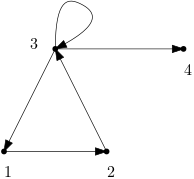
\includegraphics[width=0.3\linewidth]{img/relacije-graf.png}
            \caption{Graf relacije $R$}
        \end{figure}

        \item Naj bo $A = \NN_0$ in $R$ relacija, podana kot
        \[
            R = \{ (x,y) \in \NN_0 \times \NN_0 \mid \exists z \in \NN_0 \colon x + y = z \}.
        \]
        Ta relacija $R$ predstavlja relacijo $\leq$ na množici $\NN_0$, se pravi $(x,y) \in R \Leftrightarrow x \leq y$.

        \item V vsaki množici $A$ imamo naslednje relacije:
        \begin{itemize}
            \item $R = \emptyset \subset A \times A$. To je {\definicija prazna relacija}. V tej relaciji noben element množice $A$ ni v relaciji z nobenim drugim.
            \item $R = A \times A \subseteq A \times A$. To je {\definicija univerzalna relacija}. V tej relaciji je vsak element množice $A$ v relaciji z vsakim drugim.
            \item $R = id_A = \{ (x,x) \mid x \in A \} \subseteq A \times A$. To je {\definicija relacija enakosti}. V tej relaciji je vsak element množice $A$ v relaciji le s sabo.
        \end{itemize}
    \end{itemize}
\end{zgled}

Če je $R \subseteq A \times A$ relacija, potem namesto oznake $(x,y) \in R$ pišemo tudi $xRy$ in beremo \emph{$x$ je v relaciji $R$ z $y$}. 

Relacijo si lahko predstavljamo kot množico točk v \emph{kvadratu} $A \times A$. Za vsaka $x,y \in A$, za katera je $xRy$, označimo točko $(x,y)$ v tem kvadratu. Na ta način lahko relacijo $R$ vidimo kot neko množico točk v $A \times A$. Kot pri grafih funkcij uporabimo terminologijo, ki nam pove, kako izgleda ta množica točk. {\definicija Domena/definicijsko območje} relacije $R$ je množica
\[
    \mathcal{D}_R = \{ x \in A \mid \exists y \in A \colon x R y \},
\]
{\definicija zaloga vrednosti} relacije $R$ pa je
\[
    \mathcal{Z}_R = \{ y \in A \mid \exists x \in A \colon x R y \}.
\]

\begin{zgled} \leavevmode
    \begin{itemize}
        \item Naj bo $A = \{ 1,2,3,4 \}$ in $R = \{ (1,3), (2,2), (4,3) \}$. V tem primeru je $\mathcal{D}_R = \{1,2,3\}$ in $\mathcal{Z}_R = \{2,3\}$.
        \item Naj bo $A = \NN_0$ in $R  = \{ (x,y) \in \NN_0 \times \NN_0 \mid \exists z \in \NN_0 \colon x + z + 1 = y \}$. Relacija $R$ predstavlja relacijo $<$ v $\NN_0$. V tem primeru je $\mathcal{D}_R = \NN_0$ in $\mathcal{Z}_R = \NN$.
    \end{itemize}
\end{zgled}

Izpostavimo {\definicija nekaj lastnosti, ki jih lahko ima relacija} $R \subseteq A \times A$. Rečemo, da je relacija $R$:
\begin{itemize}
    \item {\definicija refleksivna}, če $\forall x \in A \colon x R x$,
    \item {\definicija irefleksivna}, če $\forall x \in A \colon \lnot x R x$,
    \item {\definicija simetrična}, če $\forall x,y \in A \colon (x R y \Rightarrow y R x)$,
    \item {\definicija asimetrična}, če $\forall x,y \in A \colon (x R y \Rightarrow \lnot y R x)$,
    \item {\definicija antisimetrična}, če $\forall x,y \in A \colon (xRy \land yRx \Rightarrow x = y)$,
    \item {\definicija tranzitivna}, če $\forall x,y,z \in A \colon (xRy \land yRz \Rightarrow xRz)$,
    \item {\definicija intranzitivna}, če $\forall x,y,z \in A \colon (xRy \land yRz \Rightarrow \lnot xRz)$,
    \item {\definicija strogo sovisna}, če $\forall x,y \in A \colon (xRy \lor yRx)$,
    \item {\definicija sovisna}, če $\forall x,y \in A \colon x \neq y \Rightarrow xRy \lor yRx$,
    \item {\definicija enolična}, če $\forall x,y,z \in A \colon (xRy \land xRz \Rightarrow y = z)$.
\end{itemize}

\begin{zgled} \leavevmode
    \begin{itemize}
        \item Opazujmo relacijo enakosti $=$ v množici $A$. Od naštetih lastnosti je ta relacija refleksivna, simetrična, antisimetrična, tranzitivna in enolična.
        \item Opazujmo relacijo $\leq$ v $\NN_0$. Ta relacija je refleksivna, antisimetrična, tranzitivna in strogo sovisna.
        \item Opazujmo relacijo $<$ v $\NN_0$. Ta relacija je irefleksivna, asimetrična, tranzitivna in sovisna.
        \item Opazujmo relacijo \emph{je mama} v množici ljudi. Ta relacija je irefleksivna, asimetrična, antisimetrična in intranzitivna.
    \end{itemize}
\end{zgled}

\section{Ekvivalenčne relacije}

Relacija $R \subseteq A \times A$ je {\definicija ekvivalenčna}, če je refleksivna, simetrična in tranzitivna.

\begin{zgled}
Naslednje relacije so ekvivalenčne:
\begin{itemize}
    \item relacija enakosti $=$,
    \item univerzalna relacija $A \times A$,
    \item relacija vzporednosti premic v $\RR^2$,
    \item relacija \emph{ima enako barvo oči kot} v množici ljudi,
    \item relacija \emph{ima enak BDP kot} v množici držav.
\end{itemize}
\end{zgled}

Naj bo $R \subseteq A \times A$ ekvivalenčna relacija. Vsakemu elementu $x \in A$ priredimo njegov {\definicija ekvivalenčni razred} 
\[
    R[x] = \{ y \in A \mid yRx \}.
\]
Element $x$ je {\definicija predstavnik} ekvivalenčnega razreda $R[x]$. Množico vseh ekvivalenčnih razredov označimo z
\[
    A/R = \{ R[x] \mid x \in A \}
\]
in jo imenujemo {\definicija kvocientna množica} množice $A$ po relaciji $R$.

\begin{lema}
Naj bo $R \subseteq A \times A$ ekvivalenčna relacija. Tedaj velja
\[
    \forall x,y \in A \colon (R[x] = R[y] \Leftrightarrow xRy).
\]
\end{lema}
\begin{dokaz}
Vzemimo poljubna $x,y \in A$.

$(\Rightarrow)$: Predpostavimo, da velja $R[x] = R[y]$. Ker je $R$ refleksivna relacija, velja $xRx$, torej je $x \in R[x]$. Od tod sledi $x \in R[y]$, zato je $xRy$. \kljuka

$(\Leftarrow)$: Predpostavimo, da velja $xRy$. Izberimo poljuben $z \in R[x]$. Velja torej $zRx$. Ker je $R$ tranzitivna relacija, iz $xRy$ in $zRx$ sledi $zRy$. To pomeni, da je $z \in R[y]$. Ker je bil $z$ poljuben element $R[x]$, od tod sklepamo, da velja $R[x] \subseteq R[y]$. Zaradi simetričnosti relacije $R$ lahko ponovimo ta argument, pri čemer vlogi $x$ in $y$ zamenjamo med sabo. Na ta način dobimo še vsebovanost $R[y] \subseteq R[x]$. Res torej velja $R[x] = R[y]$. \kljuka
\end{dokaz}

Iz leme v posebnem sledi, da je vsak element danega ekvivalenčnega razreda tudi njegov predstavnik.

\begin{izrek}
Naj bo $R \subseteq A \times A$ ekvivalenčna relacija. Tedaj velja:
\begin{enumerate}
    \item $\forall x \in A \colon R[x] \neq \emptyset$,
    \item $\forall x, y \in A \colon (R[x] \neq R[y] \Rightarrow R[x] \cap R[y] = \emptyset)$,
    \item $\bigcup_{x \in A} R[x] = A$.
\end{enumerate}
\end{izrek}

Povedano še drugače, ekvivalenčna relacija razdeli množico $A$ na paroma tuje neprazne bloke.

\begin{dokaz}
1. Vzemimo poljuben $x \in A$. Ker je $R$ refleksivna, velja $x R x$, zato je $x \in R[x]$. Torej je res $R[x] \neq \emptyset$. \kljuka

2. Vzemimo poljubna $x,y \in A$. Dokažimo kontrapozicijo trditve, se pravi veljavnost implikacije 
\[
    R[x]\cap R[y] \neq \emptyset \Rightarrow R[x] = R[y].
\]
Predpostavimo lahko, da obstaja $z \in R[x] \cap R[y]$. To pomeni, da velja $zRx \land zRy$. Zaradi simetričnosti $R$ sledi $xRz \land zRy$, od koder zaradi tranzitivnosti $R$ velja $xRy$. Iz leme zdaj sledi, da je $R[x] = R[y]$. \kljuka

3. Vzemimo poljuben $x \in A$. Velja $x \in R[x]$, zato je $x \in \bigcup_{y \in A} R[y]$. Ker je bil $x$ poljuben, sledi $\bigcup_{y \in A} R[y] \supseteq A$. Obratna vsebovanost je očitna. \kljuka
\end{dokaz}

\begin{zgled} \leavevmode
\begin{itemize}
    \item Naj bo $A$ množica ljudi in $R$ relacija \emph{ima enako barvo oči kot}. Ekvivalenčni razred neke osebe z modrimi očmi torej sestavljajo ravno vse osebe z modrimi očmi. Ekvivalenčni razredi torej ustrezajo barvam oči.
    \item Naj bo $A$ poljubna množica in $R$ relacija enakosti v $A$. Za vsak $x \in A$ velja $R[x] = \{ x \}$. Množica ekvivalenčnih razredov je enaka $A/R = \{ \{ x \} \mid x \in A \}$.
    \item Naj bo $A$ poljubna množica in $R$ univerzalna relacija v $A$. Za vsak $x \in A$ velja $R[x] = A$. Imamo torej en sam ekvivalenčni razred in velja $A/R = \{ A \}$.
    \item Naj bo $A$ množica premic v prostoru $\RR^3$ in naj bo $R$ relacija vzporednosti premic. Za dano premico $p$ je torej $R[p]$ ravno množica vseh premic, ki so vzporedne $p$. Ekvivalenčni razredi torej ustrezajo vsem smerem v $\RR^3$ oziroma enotskim vektorjem v $\RR^3$.
    \item Množico $\ZZ$ lahko definiramo kot kvocientno množico množice $A = \NN_0 \times \NN_0$ po relaciji $R$, kjer je $(a,b)R(c,d)$, če in samo če $a+d = b+c$. Velja $R[(a,b)] = \{ (c,d) \in \NN_0 \times \NN_0 \mid c-d = a-b \}$, zato lahko množic ekvivalenčnih razredov $A/R$ identificiramo z množico $\ZZ$ prek bijekcije $R[(a,b)] \mapsto a-b$ za $(a,b) \in A$.
    \item Naj bo $m \in \NN$. Na množici celih števil $\ZZ$ definiramo relacijo {\definicija kongruence po modulu} $m$ kot
    \[
        x \equiv y \pmod{m} \Longleftarrow \exists k \in \ZZ \mid x - y = k \cdot m.
    \]
    Elementa $x,y \in \ZZ$ sta torej kongruentna po modulu $m$, če im samo če dajeta isti ostanek pri deljenju z $m$. Ni se težko prepričati, da je to ekvivalenčni relacija. Označimo jo z $R_m$. Ekvivalenčni razredi ustrezajo ostankom pri deljenju z $m$:
    \begin{align*}
        R_m[0] &= \{ x \in \ZZ \mid \exists k \in \ZZ \colon x = k m \}, \\
        R_m[1] &= \{ x \in \ZZ \mid \exists k \in \ZZ \colon x = k m + 1 \}, \\
        \vdots \\
        R_m[m-1] &= \{ x \in \ZZ \mid \exists k \in \ZZ \colon x = k m +m-1 \}.
    \end{align*}
    Za $m = 1$ je torej $R_1 = A$, za $m = 2$ pa ima $R_2$ dva ekvivalenčna razreda, in sicer množico sodih števil in množico lihih števil.
\end{itemize}
\end{zgled}

\section{Operacije z relacijami}

Relacije v dani množici $A$ so podmnožice $A \times A$, zato lahko z njimi izvajamo vse operacije, ki jih imamo na voljo z množicami. Nekaj osnovnih takih operacij in njihovih interpretacij je zbranih v naslednji trditvi.

\begin{trditev}
Naj bosta $R,S \subseteq A \times A$ relaciji. Potem so tudi
\[
    R \cup S, \
    R \cap S, \
    R \backslash S, \
    R \oplus S
\]
relacije v $A$ in za vse $x,y \in A$ velja:
\begin{itemize}
    \item $x(R \cup S) y \Leftrightarrow x R y \lor x S y$,
    \item $x(R \cap S) y \Leftrightarrow x R y \land x S y$,
    \item $x(R \backslash S) y \Leftrightarrow x R y \land \lnot (x S y)$,
    \item $x(R \oplus S) y \Leftrightarrow x R y + x S y$.
\end{itemize}
\end{trditev}

Oglejmo si še nekaj manj poznanih operacij z relacijami. Za dano relacijo $R \subseteq A \times A$ je {\definicija komplement relacije} $R$ relacija $R^c = A \times A \backslash R$. {\definicija Transponirana relacija} relacije $R$ je relacija $R^T = \{ (x,y) \in A \times A \mid (y,x) \in R \}$. Tudi ti dve relaciji lahko intepretiramo na enostaven način.

\begin{trditev}
Za vse $x,y \in A$ velja:
    \begin{itemize}
        \item $x R^c y \Leftrightarrow \lnot (x R y)$,
        \item $x R^T y \Leftrightarrow y R x$.
    \end{itemize}
\end{trditev}

\begin{zgled}
Naj bo $A = \NN$. Med dobro poznanimi relacijami v $\NN$ veljajo naslednje enakosti:
\begin{itemize}
    \item $(<) \cup (=) = (\leq)$
    \item $(\leq) \backslash (=) = (<)$,
    \item $(\leq) \cap (\geq) = (=)$,
    \item $(\leq) \cup (\geq) = \NN \times \NN$,
    \item $(<) \cap (>) = \emptyset$,
    \item $(<) \cup (>) = (\neq) = (=)^c$,
    \item $(\leq)^c = (>)$,
    \item $(\leq)^T = (\geq)$.
\end{itemize}
\end{zgled}

Nazadnje si oglejmo še eno nekoliko bolj zapleteno operacijo. Naj bosta $R,S$ relaciji v $A$. {\definicija Kompozitum} relacij $R,S$ je relacija
\[
    R \circ S = \{ (x,y) \in A \times A \mid \exists u \in A \mid (x S u \land u R y)\}.
\]

Oglejmo si nekaj osnovnih lastnosti operacij transponiranja in kompozituma. Za vse relacije $R,S,T \subseteq A \times A$ velja:
\begin{itemize}
    \item $(R^T)^T = R$,
    \item $(R \cup S)^T = R^T \cup S^T$, \\ $(R \cap S)^T = R^T \cap S^T$, \\ $(R \backslash S)^T = R^T \backslash S^T$, \\ $(R \oplus S)^T = R^T \oplus S^T$,
    \item $R \circ id_A = R = id_A \circ R$ ({\definicija $id_A$ je enota za komponiranje}),
    \item $(R \circ S) \circ T = R \circ (S \circ T)$ ({\definicija asociativnost komponiranja}),
    \item $(R \circ S)^T = S^T \circ R^T$,
    \item $(R \cup S) \circ T = R \circ T \cup S \circ T$, \\ $R \circ (S \cup T) = R \circ S \cup R \circ T$ ({\definicija distributivnost $\circ$ glede na $\cup$}),
    \item $R \subseteq S \Rightarrow R \circ T \subseteq S \circ T$, \\ $R \subseteq S \Rightarrow T \circ R \subseteq T \circ S$ ({\definicija monotonost $\circ$ glede na $\subseteq$}).
\end{itemize}

Preverimo le zelo pomembno asociativnost komponiranja. Za vsaka $x,y \in A$ velja
\begin{align*}
    x (R \circ S) \circ T y &\Leftrightarrow \exists u \colon (xTu \land u R \circ S y) \\
    &\Leftrightarrow \exists u \colon (xTu \land \exists v \colon (uSv \land v Ry)) \\
    &\Leftrightarrow \exists u \exists v \colon (xTu \land (uSv \land vRy)) \\
    &\Leftrightarrow \exists v \exists u \colon ((xTu \land uSv) \land vRy) \\
    &\Leftrightarrow \exists v \colon (\exists u \colon ( (x T u \land uSv) \land vRy) ) \\
    &\Leftrightarrow \exists v \colon (x S \circ T v \land vRy) \\
    &\Leftrightarrow x R \circ (S \circ T) y.
\end{align*}

\begin{zgled}
Naj bo $A$ množica ljudi.
\begin{itemize}
    \item Kaj je relacija $\text{hči} \circ \text{mož}$? Za osebi $x,y \in A$ velja
    \[
        x (\text{hči} \circ \text{mož}) y \Leftrightarrow
        \exists u \colon (x \text{mož} u \land u \text{hči} y),
    \]
    torej kadar je $x$ hčerin mož $y$-a, se pravi kadar je $x$ zet $y$. Velja torej $\text{hči} \circ \text{mož} = \text{zet}$.
    \item $\text{oče} \circ \text{brat} = \text{stric}$
    \item $\text{zakonec} \circ \text{mati} = \text{tašča}$
\end{itemize}
\end{zgled}

Osnovne lastnosti relacij lahko opišemo v jeziku operacij z relacijami na naslednji način.

\begin{izrek}[algebraična karakterizacija lastnosti relacij]
Naj bo $R \subseteq A \times A$. Tedaj je:
\begin{enumerate}
    \item $R$ refleksivna, če in samo če $id_A \subseteq R$,
    \item $R$ irefleksivna, če in samo če $R \cap id_A = \emptyset$,
    \item $R$ simetrična, če in samo če $R = R^T$,
    \item $R$ asimetrična, če in samo če $R \cap R^T = \emptyset$,
    \item $R$ antisimetrična, če in samo če $R \cap R^T \subseteq id_A$,
    \item $R$ tranzitivna, če in samo če $R \circ R \subseteq R$,
    \item $R$ intranzitivna, če in samo če $(R \circ R) \cap R = \emptyset$,
    \item $R$ strogo sovisna, če in samo če $R \cup R^T = A \times A$,
    \item $R$ sovisna, če in samo če $R \cup R^T \cup id_A = A \times A$,
    \item $R$ enolična, če in samo če $R \circ R^T \subseteq id_A$.
\end{enumerate}
\end{izrek}
\begin{dokaz}
6. $(\Rightarrow)$: Predpostavimo, da je $R$ tranzitivna. Dokazati želimo, da je $R \circ R \subseteq R$. V ta namen izberimo poljuben element $(x,y) \in R \circ R$. To pomeni, da obstaja $u \in A$, za katerega velja $xRu \land uRy$. Iz tranzitivnosti relacije $R$ od tod sledi $xRy$. Slednje pomeni ravno $(x,y) \in R$. Ker je bil $(x,y)$ poljuben element $R \circ R$, smo s tem dokazali vsebovanost $R \circ R \subseteq R$. \kljuka

6. $(\Leftarrow)$: Predpostavimo, da je $R \circ R \subseteq R$. Dokazati želimo, da je $R$ tranzitivna. V ta namen predpostavimo, da za poljubne elemente $x,y,z \in A$ velja $xRy$ in $yRz$. Torej $\exists u \colon (xRu \land uRz)$, kar pomeni, da je $(x,z) \in R \circ R$. Ker je $R \circ R \subseteq R$, od tod sledi $(x,z) \in R$, se pravi $xRz$. S tem smo dokazali tranzitivnost relacije $R$. \kljuka

10. Velja 
\begin{align*}
    \text{$R$ enolična} &\Leftrightarrow \forall x,y,z \colon (xRy \land xRz \Rightarrow y=z) \\
    &\Leftrightarrow \forall x,y,z \colon (yR^Tx \land xRy \Rightarrow y = z) \\
    &\Leftrightarrow \forall y,z \colon \left( \forall x \colon (\lnot(yR^Tx \land xRy) \lor y=z) \right) \\
    &\Leftrightarrow \forall y,z \colon \left( \lnot \exists x \colon (yR^Tx \land xRy) \lor y=z \right) \\
    &\Leftrightarrow \forall y,z \colon \left( \lnot (y R \circ R^T z) \lor y = z \right) \\
    &\Leftrightarrow \forall y,z \colon (y R \circ R^T z \Rightarrow y = z) \\
    &\Leftrightarrow \forall y,z \colon \left( (y,z) \in R \circ R^T \Rightarrow y = z \right) \\
    &\Leftrightarrow R \circ R^T \subseteq id_A.
\end{align*}
\end{dokaz}

\section{Potence in ovojnice relacij}

Naj bo $R \subseteq A \times A$. {\definicija Kompozicijsko potenco} relacije $R$ definiramo induktivno na naslednji način:
\begin{description}
    \item[osnova:] $R^0 = id_A$,
    \item[indukcijski korak:] $\forall n \in \NN_0 \colon R^{n+1} = R^n \circ R^0$.
\end{description}

\begin{zgled}
Najprej velja
\[
    R^1 = R^{0+1} = R^0 \circ R = id_A \circ R = R,
\]
za tem velja
\[
    R^2 = R^{1+1} = R^1 \circ R = R \circ R
\]
in induktivno je $R^n$ enak kompoziciji $n$-tih $R$-jev. Ker je operacija komponiranja asociativna, nam pri tem ni potrebno postavljati oklepajev, saj je rezultat neodvisen od vrstnega reda izvajanja kompozicij.
\end{zgled}

Kompozicijske potence delijo nekatere lastnosti s potencami števil.

\begin{trditev}
Za vse $m,n \in \NN_0$ velja $R^n \circ R^m = R^{n+m}$ in $(R^n)^m = R^{n \cdot m}$.
\end{trditev}
\begin{dokaz}
    Vaja. Najlažje bo šlo z indukcijo na $m$.
\end{dokaz}

\begin{zgled}
Naj bo $A$ množica ljudi in $R = \text{otrok}$. Tedaj je $R^2 = \text{vnuk} \cup \text{vnukinja}$ in $R^3 = \text{pravnuk} \cup \text{pravnukinja}$ in za vsak $n \geq 2$ je
\[
    R^n = \text{(pra)$^{n-2}$vnuk} \cup \text{(pra)$^{n-2}$vnukinja}.
\]
\end{zgled}

Naj bo $R \subseteq A \times A$. S pomočjo kompozicijske potence definirajmo še dve pomembni konstrukciji, in sicer
\begin{itemize}
    \item $R^+ = \bigcup_{k = 1}^\infty R^k = R \cup R^2 \cup R^3 \cup \cdots$,
    \item $R^* = \bigcup_{k = 0}^\infty R^k = id_A \cup R \cup R^2 \cup R^3 \cup \cdots$,
\end{itemize}
Seveda velja $R^* = R^+ \cup id_A$. Relaciji $R^+$ in $R^*$ lahko opišemo še na naslednji način. Za vsaka $x,y \in A$ velja:
\begin{itemize}
    \item $x R^+ y \Leftrightarrow \exists k \in \NN \colon x R^k y$,\footnote{To pomeni, da v grafu relacije $R$ obstaja usmerjena pot dolžine vsaj $1$ od $x$ do $y$. Več o takih poteh bomo spoznali v razdelku o grafih.}
    \item $x R^+ y \Leftrightarrow \exists k \in \NN_0 \colon x R^k y$,\footnote{To pomeni, da v grafu relacije $R$ obstaja usmerjena pot od $x$ do $y$, pri čemer dopuščamo tudi možnost zanke.}
\end{itemize}

\begin{zgled}
Naj bo $A$ množica ljudi in $R = \text{otrok}$. Velja $R^+ = \text{potomec} \cup \text{potomka}$.
\end{zgled}

Nazadnje se pogovorimo še o tem, kako dano relacijo $R \subseteq A \times A$, ki ne zadošča določenim želenim lastnostim,\footnote{Na primer, $R$ morda ni refleksivna ali pa ni tranzitivna.} \emph{popraviti} do nove relacije, ki ni preveč drugačna od $R$, a za razliko od $R$ zadošča želenim lastnostim. Iščemo torej novo relacijo, ki \emph{vsebuje} relacijo $R$, ima želene lastnosti in je hkrati \emph{najmanjša} relacija med vsemi relacijami, ki imajo ti dve lastnosti.

Naj bo $\mathcal{L}$ neka lasnost relacij v množici $A$. Naj bo $R \subseteq A \times A$. Relacija $R^{\mathcal{L}}$ je {\definicija $\mathcal{L}$-ovojnica} relacije $R$, če velja:
\begin{itemize}
    \item $R \subseteq R^{\mathcal{L}}$,
    \item $R^{\mathcal{L}}$ ima lastnost $\mathcal{L}$,
    \item če ima poljubna relacija $S \subseteq A \times A$ lastnost $\mathcal{L}$ in velja $R \subseteq S$, potem je $R^{\mathcal{L}} \subseteq S$.
\end{itemize}
V primeru, ko relacija $R$ že ima lastnost $\mathcal{L}$, je seveda $R^{\mathcal{L}} = R$. V splošnem pa ovojnica $R^{\mathcal{L}}$ ne obstaja vedno. Prepričajmo se, da vselej obstajajo vsaj ovojnice glede na najbolj pomembne lastnosti relacij.

\begin{izrek}
Za vsako relacijo $R \subseteq A \times A$ obstajajo ovojnice $R^\text{refleksivnost}$, $R^\text{simetričnost}$, $R^\text{tranzitivnost}$, $R^\text{ekvivalenčnost}$ in velja:
\begin{itemize}
    \item $R^\text{refleksivnost} = R \cup id_A$ ({\definicija refleksivna ovojnica}), 
    \item $R^\text{simetričnost} = R \cup R^T$ ({\definicija simetrična ovojnica}), 
    \item $R^\text{tranzitivnost} = R^+$ ({\definicija tranzitivna ovojnica}), 
    \item $R^\text{ekvivalenčnost} = (R \cup R^T)^*$ ({\definicija ekvivalenčna ovojnica}).
\end{itemize}
\end{izrek}
\begin{dokaz}
Preverimo le trditev glede tranzitivne ovojnice. Dokazati torej želimo, da relacija $R^+$ zadošča vsem trem kriterijem v definiciji ovojnice.

Preverimo najprej, da velja $R \subseteq R^+$. Res, ker je $R^+ = R \cup R^2 \cup \cdots$, je seveda $R \subseteq R^+$. \kljuka

Prepričajmo se zdaj, da je relacija $R^+$ vselej tranzitivna. V ta namen predpostavimo, da za poljubne $x,y,z \in A$ velja $xR^+y$ in $yR^+z$. To pomeni
\[
    \exists k \in \NN \colon x R^k y \land \exists l \in \NN \colon y R^l z,
\]
kar lahko prepišemo v
\[
    \exists k, l \in \NN \colon (x R^k y \land y R^l z).
\]
Od tod sklepamo, da velja
\[
    \exists k, l \in \NN \colon (x R^l \circ R^k z),
\]
torej velja tudi
\[
    \exists m \in \NN \colon x R^m z,
\]
saj lahko vzamemo $m = k + l$. S tem smo dokazali $x R^+ z$, kar pomeni, da je relacija $R^+$ res tranzitivna. \kljuka

Nazadnje preverimo še, da je $R^+$ najmanjša tranzitivna relacija, ki vsebuje $R$. V ta namen naj bo $S$ tranzitivna relacija v $A$, za katero velja $R \subseteq S$. Dokazati želimo, da velja $R^+ \subseteq S$. Ker je $R^+ = R \cup R^2 \cup R^3 \cup \cdots$, bo za to dovolj dokazati, da za vsak $k \in \NN$ velja vsebovanost $R^k \subseteq S$. Slednje dokažimo z indukcijo na $k$.
\begin{description}
    \item[Osnova indukcije ($k = 1$):] Dokazati želimo $R \subseteq S$. To velja po predpostavki. \kljuka
    \item[Indukcijski korak ($k \to k+1$):] Predpostavimo, da velja $R^k \subseteq S$. Dokazati želimo, da velja $R^{k+1} \subseteq S$. Na predpostavki uporabimo $\circ R$ in zaradi monotonosti kompozicije dobimo $R^{k+1} = R^k \circ R \subseteq S \circ R$. Hkrati lahko na predpostavki $R \subseteq S$ uporabimo $S \circ$ in zopet iz monotonosti sledi $S \circ S \subseteq S \circ S$. Ker je $S$ tranzitivna relacija, velja $S \circ S \subseteq S$. S tem smo torej dokazali
    \[
        R^{k+1} \subseteq S \circ R \subseteq S \circ S \subseteq S,
    \]
    kar je ravno želena vsebovanost. \kljuka
\end{description}
\end{dokaz}

\begin{zgled}
Naj bo $A$ množica ljudi. Velja
\[
    \text{otrok}^\text{tranzitivnost} = \text{otrok}^+ = \text{potomec} \cup \text{potomka}.
\]
\end{zgled}

\chapter{Urejenosti}

V tem poglavju si bomo podrobneje pogledali \emph{strukture urejenosti}. To so relacije na dani množici, ki imajo določene dodatne lastnosti, s katerimi izrazimo, da te relacije podajajo \emph{ureditev} elementov dane množice. Glede na lastnosti razlikujemo več tipov urejenosti.

\section{Delna in linearna urejenost}

Naj bo $R$ relacija v $A$. Rečemo, da $R$ {\definicija delno ureja} $A$, če je $R$ refleksivna, antisimetrična in tranzitivna. Rečemo, da $R$ {\definicija linearno ureja} $A$, če $R$ delno ureja $A$ in je $R$ sovisna.

\begin{zgled} \leavevmode
\begin{itemize}
    \item Relacija $\leq$ linearno ureja realna števila $\RR$.
    \item Relacija deljivosti $|$ delno ureja naravna števila $\NN$.
    \item Naj bo $A$ neka množica množic, na primer $A = \{ B \mid B \subseteq \{ 1,2,\dots, 10\} \}$. Tedaj relacija $\subseteq$ vsebovanosti množic delno ureja $A$.
\end{itemize}
\end{zgled}

Kadar je $R$ relacija delne urejenosti, ponavadi namesto oznake $R$ pišemo kar $\leq$. Formulo $x R y$ torej zapišemo kot $x \leq y$, preberemo pa jo kot \emph{$x$ je pod $y$}.

Iz vsake relacije delne urejenosti $\leq$ v $A$ lahko konstruiramo še dve relaciji, in sicer:
\begin{itemize}
    \item {\definicija relacija stroge delne urejenosti} $<$:
    \[
        \forall x, y \in A \colon (x < y \Leftrightarrow x \leq y \land x \neq y),
        \]
    \item {\definicija relacija neposrednega predhodnika} $< \cdot$:
    \[
        \forall x, y \in A \colon \left( x < \cdot y \Leftrightarrow x < y \land \lnot \exists z \in A \colon (x < z \land z < y) \right).
    \]
\end{itemize}

Relacija $<$ je vselej irefleksivna, asimetrična in tranzitivna. Relacija $< \cdot$ je vselej irefleksivna, asimetrična in intranzitivna.

Delno urejeno množico $A$ lahko predstavimo grafično s {\definicija Hassejevim diagramom}. Elemente množice $A$ pri tem narišemo kot točke v ravnini. Če je $x < y$, potem $x$ narišemo niže od točke $y$. Če je $x < \cdot y$, potem $x$ in $y$ povežemo s črto.

\begin{zgled} \leavevmode
\begin{itemize}
    \item Naj bo $A = \{ 1,2,\dots, 10 \}$, opremljena z relacijo deljivosti naravnih števil $|$.
    
    \begin{figure}[h]
        \centering
        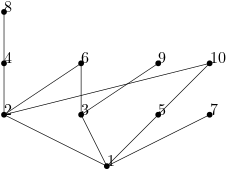
\includegraphics[width=0.5\linewidth]{img/relacije-hasse.png}
        \caption{Hassejev diagram relacije deljivosti}
    \end{figure}
    
    \item Naj bo $A = \{ B \mid B \subseteq \{ 1,2,3 \} \}$, opremljena z relacijo $\subseteq$ vsebovanosti množic.
    
    \begin{figure}[h]
        \centering
        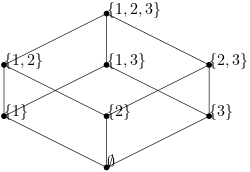
\includegraphics[width=0.5\linewidth]{img/relacije-hasse-mnozice.png}
        \caption{Hassejev diagram relacije vsebovanosti množic}
    \end{figure}

    \item Naj bo $A = \{ 1,2,3,4,5 \}$, opremljena z običajno relacijo $\leq$ (manjše ali enako).
    
    \begin{figure}[h]
        \centering
        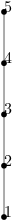
\includegraphics[height=0.5\linewidth]{img/relacije-hasse-linearna.png}
        \caption{Hassejev diagram običajne relacije $\leq$}
    \end{figure}

\end{itemize}
\end{zgled}

\section{Posebni elementi v delno urejenih množicah}

Naj relacija $\leq$ delno ureja množico $A$. Izpostavimo nekaj posebnih elementov množice $A$ glede na to delno urejenost, in sicer tiste, ki so v Hassejevem diagramu narisani tako, da pod oziroma nad njimi ni nobenega drugega elementa ali pa so celo pod oziroma nad vsemi drugimi elementi. 

Naj bo $a \in A$. Rečemo, da:
\begin{itemize}
    \item $a$ je {\definicija minimalen} v $A$, če in samo če $\forall x \in A \colon (x \leq a \Rightarrow x = a)$,
    \item $a$ je {\definicija maksimalen} v $A$, če in samo če $\forall x \in A \colon (a \leq x \Rightarrow x = a)$,
    \item $a$ je {\definicija prvi/najmanjši} v $A$, če in samo če $\forall x \in A \colon a \leq x$,
    \item $a$ je {\definicija zadnji/največji} v $A$, če in samo če $\forall x \in A \colon x \leq a$.
\end{itemize}

\begin{zgled} \leavevmode
\begin{itemize}
    \item Naj bo $A = \{ 1, 2, \dots, 10 \}$, opremljena z relacijo deljivosti $|$. Minimalni element je $1$ in to je hkrati tudi prvi element. Maksimalnih elementov je več, in sicer $7$, $10$, $9$, $6$, $8$. Zadnjih elementov pa ni.
    \item Naj bo $A = \{ B \mid B \subseteq \{ 1, 2, 3 \} \} \backslash \{ \emptyset \}$, opremljena z relacijo vsebovanosti množic $\subseteq$. Minimalni elementi so $\{ 1 \}$, $\{ 2 \}$, $\{ 3 \}$. Prvih elementov ni. Maksimalni element je $\{ 1, 2, 3 \}$ in ta je hkrati zadnji.
    \item Naj bo $A = \ZZ$, opremljena z relacijo $\leq$. Tukaj ni nobenih posebnih elementov.
    \item Naj bo $A$ poljubna množica, opremljena z relacijo $id_A$. Tukaj je vsak element maksimalen in vsak minimalen. Če ima $A$ vsaj $2$ elementa, potem ni niti prvih niti zadnjih elementov.
\end{itemize}
\end{zgled}

\begin{trditev}
Naj bo $A$ delno urejena z $\leq$.
\begin{enumerate}
    \item Vsak prvi element je minimalen.
    \item Vsak zadnji element je maksimalen.
    \item Če v $A$ obstaja prvi element, je en sam.
    \item Če v $A$ obstaja zadnji element, je en sam.
\end{enumerate}
\end{trditev}
\begin{dokaz}
1. Naj bo $a \in A$ prvi. Dokazujemo, da je $a$ minimalen. V ta namen izberimo poljuben $x \in A$, za katerega velja $x \leq a$. Dokazati želimo, da je $x = a$. Ker je $a$ prvi, velja $a \leq x$. Iz antisimetričnosti relacije $\leq$ od tod sledi $x = a$. \kljuka

2. Naj bosta $a,b \in A$ prva. Dokazati želimo, da je $a = b$. Ker je $a$ prvi, velja $a \leq b$. Ker je $b$ prvi, velja $b \leq a$. Iz antisimetričnosti relacije $\leq$ sledi $a = b$. \kljuka
\end{dokaz}

\begin{trditev}
Naj bo $A$ \emph{linearno} urejena z $\leq$.
\begin{enumerate}
    \item Element $a \in A$ je prvi, če in samo če je $a$ minimalen.
    \item Element $a \in A$ je zadnji, če in samo če je $a$ maksimalen.
\end{enumerate}
\end{trditev}
\begin{dokaz}
1. Po prejšnji trditvi bo dovolj dokazati implikacijo $(\Leftarrow)$. Naj bo torej $a \in A$ minimalen. Dokazati želimo, da je $a$ prvi. V ta namen izberimo poljuben $x \in A$. Dokazati želimo, da je $a \leq x$. Linearna urejenost je strogo sovisna, zato velja $a \leq x$ ali $x \leq a$. Uporabimo analizo primerov. 
\begin{itemize}
    \item Če je $a \leq x$, potem želeno velja. \kljuka 
    \item Če je $x \leq a$, iz minimalnosti $a$ sledi $x = a$, torej velja tudi $a \leq x$. \kljuka.
\end{itemize}
\end{dokaz}

Naj bo množica $A$ delno urejena z relacijo $R$ in naj bo $B \subseteq A$ poljubna podmnožica $A$. V tem primeru lahko relacijo $R$ {\definicija zožimo} na množico $B$ in dobimo relacijo
\[
    R |_B = R \cap (B \times B) \subseteq B \times B
\]
v množici $B$. Na ta način lahko govorimo o minimalnih, maksimalnih, prvih in zadnjih elementih množice $B$ glede na relacijo $R|_B$.
\begin{itemize}
    \item Če ima $B$ prvi element, ga imenujemo {\definicija minimum} množice $B$ in označimo z $\min B$.
    \item Če ima $B$ zadnji element, ga imenujemo {\definicija maksimum} množice $B$ in označimo z $\max B$.
    \item Element $a \in A$ je {\definicija zgornja meja} za $B$, če $\forall x \in B \colon \; x \leq a$.
    \item Element $a \in A$ je {\definicija spodnja meja} za $B$, če $\forall x \in B \colon \; a \leq x$.
\end{itemize}

\begin{zgled} \leavevmode
\begin{itemize}
    \item Naj bo $A = \RR$, opremljena z relacijo $\leq$. Naj bo $B = (0,1)$ odprti interval. Tedaj $\min B$ in $\max B$ ne obstajata. Vsako število $a \geq 1$ je zgornja meja za $B$ in vsako število $a \leq 0$ je spodnja meja za $B$.
    \item Naj bo $A = \NN$, opremljena z relacijo deljivosti $|$. Naj bo $B = \{ 12, 18, 24, 72 \}$. Tedaj $\min B$ ne obstaja, $\max B$ pa je enak $72$. Vsako število oblike $72k$ za $k \in \NN$ je zgornja meja za $B$. Števila $1$,$2$,$3$,$6$ so spodnje meje za $B$.
\end{itemize}
\end{zgled}

Med vsemimi zgornjimi oziroma spodnjimi mejami včasih obstajajo najmanjše oziroma največje take meje. Za te uvedemo posebno ime.
\begin{itemize}
    \item Naj bo $M$ množica vseh zgornjih mej za $B$, se pravi
    \[
        M = \{ a \in A \mid \forall x \in B \colon \; x \leq a \}.
    \]
    Če ima $M$ prvi element, ga imenujemo {\definicija supremum} ali {\definicija najmanjša zgornja meja} množice $B$ in označimo s $\sup B$.
    
    \item Naj bo $m$ množica vseh spodnjih mej za $B$, se pravi
    \[
        m = \{ a \in A \mid \forall x \in B \colon \; a \leq x \}.
    \]
    Če ima $m$ zadnji element, ga imenujemo {\definicija infimum} ali {\definicija največja spodnja meja} množice $B$ in označimo s $\inf B$.
\end{itemize}

\begin{zgled} \leavevmode
    \begin{itemize}
        \item Naj bo $A = \RR$, opremljena z običajno relacijo $\leq$. Naj bo $B = (0,1)$. Velja
        $\inf B = 0$ in $\sup B = 1$.
        \item Naj bo $A = \NN$, opremljena z relacijo deljivosti $|$. Naj bo $B = \{ 12, 18, 24, 72 \}$. Tedaj je infimum $\inf B$ enak največjemu skupnemu delitelju $D(12, 18, 24, 72) = 6$, supremum $\sup B$ pa je enak najmanjšemu skupnemu večkratniku $v(12, 18, 24, 72) = 72$.
        \item Infimum in supremum ne obstajata vedno. Na primer, če vzamemo $A = \RR$ z relacijo $\leq$ in $B = \{ n \mid n \in \NN \}$, potem množica $B$ nima zgornjih mej v množici $A$, torej je $M = \emptyset$. Prazna množica seveda nima prvega elementa, torej množica $B$ nima supremuma.
    \end{itemize}
\end{zgled}

Kadar ima množica $B$ zadnji element, je ta seveda enak $\sup B$. Sorodno velja v primeru, ko ima $B$ prvi element, takrat je ta enak $\inf B$.

\section{Mreža}

Nazadnje si na hitro oglejmo še eno strukturo urejenosti, ki leži vmes med delno urejenostjo in linearno urejenostjo.

Delno urejena množica $A$ je {\definicija mreža}, če za vsaka dva elementa $a,b \in A$ obstajata $\inf \{ a, b \}$ in $\sup \{ a, b \}$.

\begin{zgled} \leavevmode
    \begin{itemize}
        \item Vsaka linearno urejena množica $A$ je mreža. Res, za vsaka $a,b \in A$ velja $\inf \{ a, b \} = \min \{ a,b \}$ in $\sup \{ a, b \} = \max \{ a, b \}$ in tako minimum kot maksimum obstajata, ker je $A$ linearno urejena in zato v posebnem sovisna.
        \item Naj bo $A = \NN$, opremljena z relacijo deljivosti $|$. Ta delno urejena množica je mreža, saj za vsaka $a, b \in \NN$ velja $\inf \{ a,b \} = D(a,b)$ in $\sup \{ a, b \} = v(a,b)$.
        \item Naj bo $S$ poljubna neprazna množica in naj bo $A$ množica podmnožic $S$, se pravi $A = \{ B \mid B \subseteq S \}$, opremljena z relacijo vsebovanosti množic $\subseteq$. Ta delno urejena množica je mreža, saj za vsaki množici $B, C \in A$ velja $\inf \{ B, C \} = B \cap C$ in $\sup \{ B, C \} = B \cup C$.
        \item Zadnji zgled modificirajmo tako, da za množico $A$ vzamemo le \emph{neprazne} podmnožice množice $S$. To je še vedno delno urejena množica. Za različna elementa $x,y \in S$ infimum $\inf \{ \{ x \}, \{ y \} \}$ \emph{ne} obstaja. To torej ni mreža.
    \end{itemize}
\end{zgled}

\emph{Linearna urejenost} je torej poseben primer \emph{mreže}, ta pa je poseben primer \emph{delne urejenosti}.

\chapter{Grafi}

Diskretne strukture, ki smo jih obravnavali do sedaj (torej relacije), so izhajale iz našega študija izjavnega in predikatnega računa. Ogledali smo si že, kako lahko relacije predstavimo z  \emph{grafom relacije}. V tem zadnjem razdelku bomo ta abstrakten objekt, \emph{graf}, obravnavali neodvisno. Ta diskretna struktura je zelo pogosta v različnih področjih matematike, še posebej v njenih aplikacijah v resničnem svetu. Ogledali si bomo nekaj lastnosti te strukture in dokazali nekaj osnovnih izrekov o njej. 

\section{Osnovne definicije}

{\definicija Graf} $G$ je par množic $(V,E)$, kjer je $V$ neka končna\footnote{Mi se bomo omejili le na končne grafe, v matematiki pa sicer obravnavamo tudi neskončne grafe.} neprazna množica, $E$ pa je neka množica dvoelementnih podmnožic\footnote{Spomnimo se, da je relacija na množici $V$ podmnožica množice $V \times V$, torej sestoji iz \emph{urejenih} parov elementov iz $V$. Po drugi strani pa množica $E$ sestoji iz \emph{neurejenih parov} elementov iz $V$, se pravi iz podmnožic $V$ z dvema elementoma.} množice $V$. Množici $V$ pravimo {\definicija množica točk/vozlišč grafa}, množici $E$ pa pravimo {\definicija množica povezav grafa}.

\begin{zgled}
Naj bo $V = \{ 1, 2, 3, 4, 5 \}$ in naj bo
\[
    E = \{  
        \{ 1, 2 \}, 
        \{ 2, 3 \},
        \{ 3, 4 \},
        \{ 4, 1 \},
        \{ 1, 3 \},
        \{ 4, 5 \}
         \}.
\]

Graf $G = (V,E)$ si lahko vizualiziramo tako, da vozlišča narišemo kot točke v ravnini, za tem pa vozlišči $u,v \in V$ povežemo, če in samo če je $\{ u, v \} \in E$.

\begin{figure}[h]
    \centering
    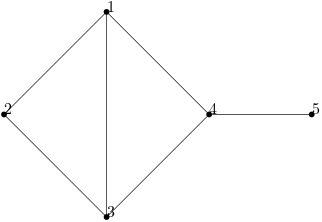
\includegraphics[width=0.5\linewidth]{img/grafi-prvizgled.png}
    \caption{Zgled vizualizacije grafa}
\end{figure}

\end{zgled}

Kadar za vozlišči $u,v \in V$ velja $\{ u, v \} \in E$, potem rečemo, da sta vozlišči $u,v$ {\definicija sosednji} in pišemo $u \sim v$. Povezavo $\{ u, v \} \in E$ včasih pišemo krajše kot $uv$.

Včasih definicijo grafa nekoliko omehčamo do te mere, da dopustimo obstoj {\definicija vzporednih povezav} (to pomeni, da med istim parom točk obstaja več povezav) in {\definicija zank} (to so povezave, ki imajo obe krajišči enaki). Takim splošnejšim strukturam rečemo {\definicija multigrafi}.

\begin{zgled}
    \begin{figure}[h]
        \centering
        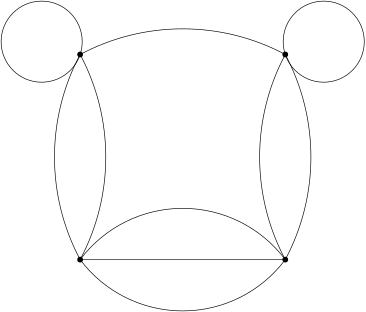
\includegraphics[width=0.5\linewidth]{img/grafi-multigraf.png}
        \caption{Zgled multigrafa}
    \end{figure}
\end{zgled}

Naj bo $G = (V,E)$ graf in $u \in V$. {\definicija Stopnja točke} $u$ je število povezav v $E$, ki imajo $u$ za svoje krajišče. Stopnjo označimo kot $\deg_G(u)$ ali krajše kot $d(u)$. Točkam stopnje $0$ pravimo {\definicija izolirane točke}, točkam stopnje $1$ pa {\definicija listi}.

\begin{zgled}
Naj bo $G$ graf, predstavljen na naslednji sliki.

\begin{figure}[h]
    \centering
    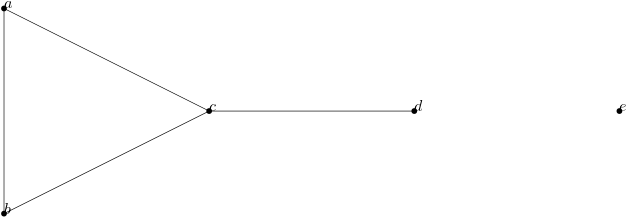
\includegraphics[width=0.75\linewidth]{img/grafi-std-izolirana.png}
    \caption{Graf z listom in izolirano točko}
\end{figure}

Stopnje vozlišč so $d(a) = 2$, $d(b) = 2$, $d(c) = 3$, $d(d) = 1$, $d(e) = 0$. Vozlišče $d$ je list, vozlišče $e$ pa je izolirana točka.
\end{zgled}

Najmanjšo stopnjo vozlišča označimo z
\[
    \delta(G) = \min \{ d(u) \mid u \in V \},
\]
največjo stopnjo pa označimo z 
\[
  \Delta(G) = \max \{ d(u) \mid u \in V \}. 
\]
Graf je {\definicija regularen}, če je $\delta(G) = \Delta(G)$, torej če imajo vsa vozlišča enako stopnjo. Če je ta stopnja $d$, rečemu grafu {\definicija $d$-regularen}.

\begin{zgled} \leavevmode
\begin{itemize}
    \item
    \begin{figure}[h]
        \centering
        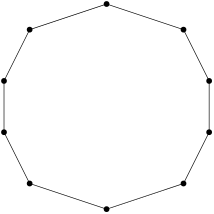
\includegraphics[width=0.5\linewidth]{img/grafi-2reg.png}
        \caption{Zgled $2$-regularnega grafa}
    \end{figure}

    \item
    \begin{figure}[h]
        \centering
        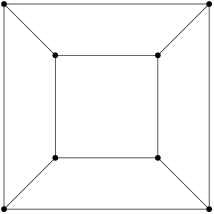
\includegraphics[width=0.5\linewidth]{img/grafi-3reg.png}
        \caption{Zgled $3$-regularnega grafa}
    \end{figure}

    \item
    \begin{figure}[h]
        \centering
        \includegraphics[width=0.5\linewidth]{img/opis-petersen.png}
        \caption{Petersenov graf je $3$-regularen}
    \end{figure}
\end{itemize}
\end{zgled}

Grafe lahko ekvivalentno opišemo s pomočjo matrik. Za to imamo na voljo dve možnosti.

Prva možnost je {\definicija matrika sosednosti} grafa $G$. Za njeno konstrukcijo najprej oštevilčimo množico vozlišč $V = \{ v_1, v_2, \dots, v_n \}$ in nato sestavimo matriko $A(G) = [a_{ij}]_{1 \leq i,j \leq n}$ z vnosi
\[
    a_{ij} = \begin{cases}
        1 & v_i \sim v_j \\
        0 & \text{sicer.}
    \end{cases}
\]

\begin{zgled}
Naj bo $G$ graf, predstavljen na naslednji sliki. Ta graf bomo srečali še večkrat, zato mu dajmo ime {\definicija lizika}.

\begin{figure}[h]
    \centering
    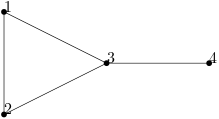
\includegraphics[width=0.5\linewidth]{img/grafi-std.png}
    \caption{Lizika}
\end{figure}

Matrika sosednosti lizike je 
\[
    A(G) = \begin{pmatrix}
        0 & 1 & 1 & 0 \\
        1 & 0 & 1 & 0 \\
        1 & 1 & 0 & 1 \\
        0 & 0 & 1 & 0
    \end{pmatrix}.
\]
Opazimo, da je ta matrika simetrična. To ni slučaj, saj za vsaka $i,j$ velja $a_{ij} = 1$, če in samo če je $v_i \sim v_j$, torej če in samo če je $a_{ji} = 1$.
\end{zgled}

Druga možnost je {\definicija incidenčna matrika} grafa $G$. Za njeno konstrukcijo najprej oštevilčimo množico vozlišč $V = \{ v_1, v_2, \dots, v_n \}$ in povezav $E = \{ e_1, e_2, \dots, e_m \}$ in nato sestavimo matriko $B(G) = [b_{ij}]_{1 \leq i \leq n, 1 \leq j \leq m}$ z vnosi
\[
    b_{ij} = \begin{cases}
        1 & v_i \in e_j \\
        0 & \text{sicer.}
    \end{cases}
\]

\begin{zgled}
Opazujmo liziko. Povezave označimo kot $e_1 = \{ 1, 2 \}$, $e_2 = \{ 1, 3 \}$, $e_3 = \{ 2, 3 \}$ in $e_4 = \{ 3, 4 \}$. Incidenčna matrika je 
\[
    B(G) =
    \begin{pmatrix}
        1 & 1 & 0 & 0 \\
        1 & 0 & 1 & 0 \\
        0 & 1 & 1 & 1 \\
        0 & 0 & 0 & 1
    \end{pmatrix}.
\]
Ta matrika ni simetrična. V splošnem to niti ni kvadratna matrika, saj je število vozlišč grafa lahko različno od števila povezav.
\end{zgled}

Vsak stolpec incidenčne matrike vsebuje natanko dve enici, ker ima vsaka povezava natanko dve krajišči. Torej je vsota vseh členov matrike $B(G)$ enaka dvakratniku števila povezav, se pravi $2 |E|$. Po drugi strani pa je število enic v $i$-ti vrstici matrike $B(G)$ enako stopnji $d(v_i)$. Torej je vsota vseh členov matrike $B(G)$ enaka vsoti stopenj vseh vozlišč grafa. Na ta način smo izpeljali naslednjo elementarno, a pomembno lastnost grafov.

\begin{lema}[o rokovanju]
    Za vsak graf $G = (V,E)$ velja
    \[
        \sum_{v \in V} d(v) = 2 |E|.
    \]
\end{lema}

\begin{zgled} \leavevmode
    \begin{itemize}
        \item Petersenov graf je $3$-regularen graf na $10$ vozliščih. Iz leme o rokovanju sklepamo, da je $10 \cdot 3 = 2 \cdot |E|$, torej ima Petersenov graf $15$ povezav. Ta sklep velja za vsak $3$-regularen graf na $10$ vozliščih.
        \item Ali obstaja $3$-regularen graf na $9$ vozliščih? Če bi obstajal, potem bi po lemi o rokovanju veljalo $9 \cdot 3 = 2 \cdot |E|$, torej je $|E| = 27/2$, kar ni mogoče. Tak graf torej ne obstaja.
    \end{itemize}
\end{zgled}

\begin{posledica}
Vsak graf ima sodo mnogo točk lihe stopnje.
\end{posledica}
\begin{dokaz}
Naj bo $G = (V,E)$ graf. Po lemi o rokovanju je $\sum_{v \in V} d(v)$ sodo število. Naj bo $V^0 = \{ v \in V \mid \text{$d(v)$ je sodo} \}$ in $V^1 = \{ v \in V \mid \text{$d(v)$ je liho} \}$. Torej je 
\[
    \sum_{v \in V^0} d(v) + \sum_{v \in V^1} d(v)
\]
sodo število. Ker so v prvi vsoti vsi členi $d(v)$ sodi, mora biti druga vsota soda. Vsak člen v drugi vsoti pa je lih, zato mora biti velikost množice $V^1$ soda. S tem je dokaz zaključen.
\end{dokaz}

Graf $H$ je {\definicija podgraf} grafa $G$, če velja $V(H) \subseteq V(G)$ in $E(H) \subseteq E(G)$. V tem primeru pišemo $H \subseteq G$. Rečemo tudi, da graf $G$ {\definicija vsebuje} graf $H$. Podgraf $H$ je {\definicija vpet}, če velja $V(H) = V(G)$.

\begin{zgled}
Naj bo $G$ lizika z vozlišči $V(G) = \{ 1,2,3,4 \}$. Naj bo $H$ graf z vozlišči $V(H) = \{ 1,2,3,4 \}$ in povezavami $E(H) = \emptyset$. Tedaj je $H$ vpet podgraf grafa $G$.
\end{zgled}

\section{Standardni primeri in operacije}

V tem razdelku si bomo ogledali nekaj standardnih primerov grafov in elementarne operacije, ki jih lahko izvajamo na njih, da dobimo nove grafe.

\subsection{Standardni primeri}

Naj bo $n \in \NN$ in naj bo $\ZZ/n\ZZ$ kvocientna množica množice $\ZZ$ po relaciji $\mod{n}$. Elemente množice $\ZZ/n\ZZ$ lahko torej identificiramo z ostanki pri deljenju z $n$, se pravi s števili $0, 1, \dots, n-1$. Te ostanke lahko tudi seštevamo (po modulu $n$).\footnote{Na primer $3 + 7 \equiv 1 \pmod{9}$.} S pomočjo množice $\ZZ/n\ZZ$ bomo definirali nekaj osnovnih primerov grafov.

\begin{itemize}
    \item {\definicija Poln graf} $K_n$ ima vozlišča in povezave 
\[
    V = \ZZ/n\ZZ, \quad
    E = \{ \{ u,v \} \mid u,v \in \ZZ/n\ZZ, \ u \neq v \}.
\]
Ta graf ima $n$ vozlišč in $\binom{n}{2}$ povezav. Je $(n-1)$-regularen graf.

    \item {\definicija Pot} $P_n$ ima vozlišča in povezave
\[
    V = \ZZ/n\ZZ, \quad
    E = \{ \{ u, u+1 \} \mid u \in \{ 0, 1, \dots, n-2 \}.
\]
Ta graf ima $n$ vozlišč in $n-1$ povezav. Rečemo, da je {\definicija dolžina} poti $P_n$ enaka $n-1$.

    \item {\definicija Cikel} $C_n$ (definiran le za $n \geq 3$) ima vozlišča in povezave
\[
    V = \ZZ/n\ZZ, \quad
    E = \{ \{ u, u+1 \} \mid u \in \ZZ/n\ZZ \}.
\]
Ta graf ima $n$ vozlišč in $n$ povezav. Je $2$-regularen graf.
\end{itemize}

Nekaj dodatnih primerov grafov bomo uvedli s pomočjo naslednje lastnosti grafov. Graf $G = (V,E)$ je {\definicija dvodelen}, če lahko množico vozlišč $V$ zapišemo kot disjunktno unijo $V = A \cup B$, $A \cap B = \emptyset$, pri čemer mora za vsako povezavo v $E$ biti eno krajišče v $A$, drugo pa v $B$.\footnote{Vozlišča grafa lahko torej razdelimo na dva dela, pri čemer povezave v grafu potekajo le med vozlišči iz različnih delov.}

\begin{zgled} \leavevmode
    \begin{itemize}
        \item Poln graf $K_n$ ni dvodelen graf za $n \geq 3$.
        \item Pot $P_n$ je dvodelen graf za $n \geq 2$, saj lahko množico $\ZZ/n\ZZ$ zapišemo kot unijo sodih števil ($A$) in lihih števil ($B$) med $0$ in $n-1$, povezave v $P_n$ pa vedno tečejo le med sodimi in lihimi števili.
        \item Cikel $C_n$ je dvodelen graf, če je $n$ sodo število. V tem primeru lahko namreč uporabimo enak argument kot za pot $P_n$, saj lahko $\ZZ/n\ZZ$ razdelimo na soda in liha števila in vse povezave v $C_n$ tečejo le med sodimi in lihimi števili. 
        
        Ta argument pa ne deluje, ko je $n$ liho število, saj takrat dobimo še dodatno povezavo med sodima številoma $0 \sim n-1$. Prepričajmo se, da cikel $C_n$ za $n$ lih \emph{ni} dvodelen. Res, denimo, da je z razčlenitvijo vozlišč $V = A \cup B$. Brez škode lahko predpostavimo, da je $0 \in A$. Potem je nujno $1 \in B$ in za tem $2 \in A$ in za tem $3 \in B$ in tako dalje vse do $n-1 \in A$, saj je $n$ liho. Ker pa je $0 \sim n-1$ v ciklu $C_n$, dobimo povezavo dveh vozlišč v množici $A$, kar je sprto s predpostavko o dvodelnosti grafa. Lihi cikli torej niso dvodelni.
    \end{itemize}
\end{zgled}

Ni se težko prepričati, da je obstoj lihih ciklov v grafu \emph{edina} obstrukcija k dvodelnosti grafa.

\begin{trditev}
Graf je dvodelen natanko tedaj, ko ne vsebuje lihega cikla.
\end{trditev}
\begin{dokaz}
$(\Rightarrow)$: Naj bo $G$ dvodelen graf. Tedaj je vsak njegov podgraf tudi dvodelen. Ker lihi cikli niso dvodelni, jih $G$ ne more vsebovati. \kljuka

$(\Leftarrow)$: Predpostavimo, da $G$ ne vsebuje lihega cikla. Naj bo $v \in V(G)$ poljubno začetno vozlišče. Za vozlišče $u \in V(G)$ naj bo $d(v,u)$ najmanjše število povezav, ki jih potrebujemo, da od vozlišča $v$ pridemo do vozlišča $u$.\footnote{Kasneje bomo številu $d(v,u)$ rekli tudi dolžina najkrajše poti od $v$ do $u$. Lahko se zgodi, da je od $v$ sploh ne moremo priti do $u$, na primer če je $u$ izolirana točka. V tem primeru definiramo $d(v,u) = \infty$.} Vozlišča $u$, za katera je $d(v,u)$ sodo število, obarvamo z rdečo, vozlišča $u$, za katera je $d(v,u)$ liho število, pa obarvamo z modro.\footnote{Če je $d(v,u) = \infty$, potem vozlišča $u$ zaenkrat ne obarvamo.} Naj bo $A$ množica vseh rdečih vozlišč, $B$ pa množica modrih vozlišč.

Predpostavimo, da je $\{ u, w \}$ povezava v $G$, za katero je $u, w \in B$.\footnote{Analogen argument deluje, če sta obe krajišči v $A$.} Torej sta $d(v,u)$ in $d(v,w)$ oba liha. V grafu $G$ lahko torej pridemo od vozlišča $v$ do $u$ po liho povezavah in prav tako od vozlišča $v$ do $w$ po liho povezavah. V grafu $G$ lahko torej začnemo pri vozlišču $v$ in po liho korakih pridemo do $u$, za tem prečkamo povezavo $uw$ in nato nadaljujemo od $w$ do $v$. Skupaj se sprehodimo po liho mnogo povezavah.\footnote{Pri tem morda kakšno vozlišče sicer obiščemo več kot enkrat, zato to morda ni podgraf $G$.} Nekoliko kasneje bomo premislili, da ima vsak graf z obhodom lihe dolžine tudi lih cikel. Ker pa lihih ciklov v $G$ po predpostavki ni, smo dosegli protislovje s predpostavko, da v $G$ obstajajo povezave med vozlišči v množici $B$ oziroma v množici $A$. Takih povezav torej ni in graf $G$ je dvodelen.\footnote{Natančneje, podgraf grafa $G$, vpet v vozlišča $u$, za katera velja $d(v,u) < \infty$, je dvodelen. Če obstaja kakšno vozlišče z $d(v,u) = \infty$, zdaj vzamemo to vozlišče za začetno in ponovimo opisan postopek.}
\end{dokaz}

\begin{itemize}
    \item {\definicija Poln dvodelni graf} $K_{m,n}$ ima vozlišča in povezave
\[
    V = A \cup B, |A| = m, |B|=n, A \cap B = \emptyset, \quad
    E = \{ \{ u,v\} \mid u \in A, v \in B \}.
\]
V tem grafu so torej vsa vozlišča množice $A$ povezana z vsemi vozlišči množice $B$. Ta graf ima $m+n$ vozlišč in $m \cdot n$ povezav. 

    \item Grafom $K_{1,n}$ za $n \geq 3$ pravimo {\definicija zvezde}.

    \item {\definicija Kolo} $W_n$ (definiran le za $n \geq 3$) ima vozlišča in povezave
\[
    V = \ZZ/n\ZZ \cup \{ \infty \}, \quad
    E = \{ \{ u, u+1 \} \mid u \in \ZZ/n\ZZ \} \cup \{ \{ u, \infty \} \mid u \in \ZZ/n\ZZ \}.
\]
Ta graf ima $n+1$ vozlišč in $2n$ povezav.
\end{itemize}

\subsection{Operacije}

Oglejmo si zdaj še nekaj osnovnih operacij, ki jih lahko izvedemo na danem grafu oziroma grafih.

\begin{itemize}
    \item {\definicija Odstranjevanje vozlišč}. Dan je graf $G = (V,E)$ in $u \in V$. Graf $G - u$ ima vozlišča in povezave
    \[
        V(G - u) = V \backslash \{ u \}, \quad
        E(G - u) = \{ e \in E \mid u \notin e \}.
    \]

    \item {\definicija Odstranjevanje povezav}. Dan je graf $G = (V,E)$ in $e \in E$. Graf $G - e$ ima vozlišča in povezave
    \[
        V(G - e) = V, \quad
        E(G - e) = E \backslash \{ e \}.   
    \]

    \item {\definicija Komplementiran graf}. Dan je graf $G = (V,E)$. Graf $\bar G$ ima vozlišča in povezave
    \[
        V(\bar G) = V, \quad
        E(\bar G) = \{ \{ u,v \} \mid u,v \in V, \{ u,v \} \notin E \}.
    \]

    \item {\definicija Unija grafov}. Dana sta grafa $G_1, G_2$. Graf $G_1 \cup G_2$ ima vozlišča in povezave
    \[
        V(G_1 \cup G_2) = V(G_1) \cup V(G_2), \quad 
        E(G_1 \cup G_2) = E(G_1) \cup E(G_2).
    \]
\end{itemize}

\section{Invariante grafov}

Dana sta grafa $G_1, G_2$, ki sicer na prvi pogled izgledata drugače, a če ustrezno oštevilčimo vozlišča obeh grafov, potem vidimo, da povezave v obeh grafih potekajo med natanko istimi pari vozlišč. V tem primeru lahko \emph{identificiramo} ta dva grafa. Natančneje, preslikava $h \colon V(G_1) \to V(G_2)$ je {\definicija izomorfizem grafov}, če je $h$ bijekcija in velja
\[
    \forall u,v \in V(G_1) \colon 
    \left( \{ u,v \} \in E(G_1) \Leftrightarrow \{ h(u), h(v) \} \in E(G_2) \right).
\]
V tem primeru rečemo, da sta grafa $G_1$ in $G_2$ {\definicija izomorfna} in pišemo $G_1 \cong G_2$. V posebnem primeru, ko je $G_1 = G_2$, izomorfizmu grafov $h$ pravimo {\definicija avtomorfizem grafa} $G_1$.

\begin{zgled} \leavevmode
    \begin{itemize}
        \item Za vsak graf $G$ je preslikava
        \[
            h \colon V(G) \to V(G), \quad 
            u \mapsto u  
        \]
        avtomorfizem grafa $G$. Pravimo mu {\definicija trivialni avtomorfizem}.

        \item Naj bo $G = C_n$ cikel dolžine $n$. Ta cikel lahko \emph{zavrtimo} za $1$ v smeri urinega kazalca. Natančneje, definirajmo preslikavo
        \[
            h \colon \ZZ/n\ZZ \to \ZZ/n\ZZ, \quad
            u \mapsto u + 1.
        \]
        Za vsaki vozlišči $u,v \in \ZZ/n\ZZ$ velja
        \[
            \{ u,v \} \in E(C_n) \Leftrightarrow v = u \pm 1 \pmod{n}
        \]
        in
        \[
            \{ h(u), h(v) \} \in E(C_n) \Leftrightarrow h(v) = h(u) \pm 1 \pmod{n}
            \Leftrightarrow v = u \pm 1 \pmod{n}.
        \]
        Preslikava $h$ je torej avtomorfizem grafa $C_n$.

        \item Naj bo $G_1 = C_6$ cikel dolžine $6$ in $G_2$ graf z vozlišči in povezavami
        \[
            V(G_2) = \{ a,b,c,d,e,f \}, \quad
            E(G_2) = \{ ad, ae, bd, bf, ce, cf \}.
        \]
        Prepričajmo se, da sta grafa $G_1$ in $G_2$ izomorfna. Definirajmo preslikavo
        \[
            h \colon V(G_1) \to V(G_2), \quad
            0 \mapsto d, 1 \mapsto a, 2 \mapsto e, 3 \mapsto c, 4 \mapsto f, 5 \mapsto b.
        \]
        Za vsaka $i,j \in V(G_1)$ velja $i \sim j$, če in samo če $h(i) \sim h(j)$. Preslikava $h$ je torej izomorfizem grafov.
    \end{itemize}
\end{zgled}

Kako bi dokazali, da dana grafa \emph{nista} izomorfna? V tem primeru ponavadi uporabimo kakšno lastnost grafov (na primer število povezav, dvodelnost), ki se pri izomorfizmu ohranja. Natančneje, naj bo $\mathcal{L}$ neka lastnost grafov. Rečemo, da je $\mathcal{L}$ {\definicija invarianta grafa}, če za vsaka dva izomorfna grafa $G_1, G_2$ velja, da ima $G_1$ lastnost $\mathcal{L}$ natanko tedaj, ko ima $G_2$ lastnost $\mathcal{L}$.

\begin{zgled}
    Invariante grafov so število točk, število povezav, dvodelnost, število točk stopnje $3$, število trikotnikov, \dots
\end{zgled}

Če želimo dokazati, da dana grafa nista izomorfna, lahko torej poiščemo kakšno invarianto, v kateri se obravnavana grafa razlikujeta.

\begin{zgled} \leavevmode
    \begin{itemize}
        \item Naj bo $L$ lizika in $C_4$ cikel. Lizika ima vozlišče stopnnje $3$, cikel pa je $2$-regularen. Ta dva grafa torej nista izomorfna.
        
        \item Dana sta naslednja grafa $G_1$ in $G_2$.
        
        \begin{figure}[h]
            \centering
            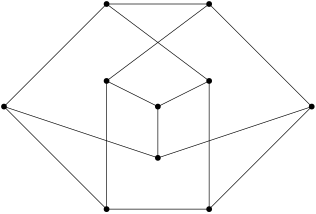
\includegraphics[width=0.5\linewidth]{img/grafi-zanimiv-zgled.png}
            \caption{Graf $G_1$}
        \end{figure}

        \begin{figure}[h]
            \centering
            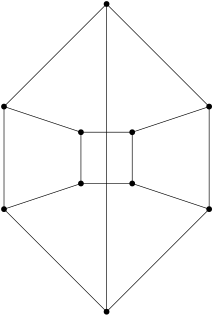
\includegraphics[width=0.5\linewidth]{img/grafi-primerjava.png}
            \caption{Graf $G_2$}
        \end{figure}

        Ali sta $G_1$ in $G_2$ izomorfna? Ujemata se v številu vozlišč in številu povezav. Oba vsebujeta $5$-cikel, zato nista dvodelna. Oba sta kubična grafa. Noben od grafov ne vsebuje trikotnika. Ta dva grafa pa se razlikujeta v dolžini najkrajšnega cikla v grafu, ki ji pravimo {\definicija ožina grafa}. Ožina je seveda invarianta grafov. Ožina grafa $G_1$ je $5$, ožina grafa $G_2$ pa je $4$. Ta dva grafa torej nista izomorfna.
    \end{itemize}
\end{zgled}

Poglejmo si še nekaj invariant grafov, ki temeljijo na opazovanju \emph{poti}. Naj bo $G = (V,E)$ graf. 

\begin{itemize}
    \item {\definicija Sprehod} v $G$ je zaporedje
    \[
        v_0 e_1 v_1 e_2 v_2 \cdots v_{k-1} e_k v_k,
    \]
    kjer je $v_i \in V$, $e_i = \{ v_{i-1}, v_i \} \in E$. Pri tem številu $k$ pravimo {\definicija dolžina sprehoda}. Pogosto izpustimo podatke o povezavah in zapišemo le zaporedje vozlišč $v_0 v_1 v_2 \dots v_k$.

    \item {\definicija Obhod} je sklenjen sprehod, se pravi $v_0 = v_k$.
    \item {\definicija Enostaven sprehod} je sprehod, v katerem so vse \emph{povezave} različne med sabo.
    \item {\definicija Pot} je enostaven sprehod, v katerem so vsa \emph{vozlišča} različna med sabo.
    \item {\definicija Cikel} je enostaven obhod, v katerem so vozlišča $v_0, v_1, \dots, v_{k-1}$ različna med sabo.
\end{itemize}

\begin{zgled}
    V naslednjem grafu je označen primer poti in primer cikla.
    \begin{figure}[h]
        \centering
        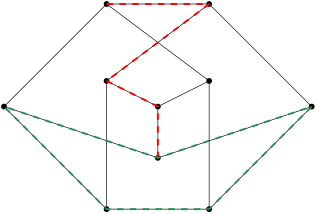
\includegraphics[width=0.5\linewidth]{img/grafi-pot-cikel.png}
        \caption{Graf z rdečo potjo in zelenim ciklom}
    \end{figure}
\end{zgled}

Ni vsak sprehod pot. Je pa povsod, kjer je sprehod, tudi pot.

\begin{trditev}
Če v grafu obstaja sprehod od $u$ do $v$, potem obstaja tudi pot od $u$ do $v$.
\end{trditev}
\begin{dokaz}
Dokazujemo z indukcijo na dolžino sprehoda $k$.

Baza indukcije je $k = 1$. V tem primeru je sprehod kar enak $P_2$, kar je pot. \kljuka

Predpostavimo zdaj, da trditev že velja za vse sprehodi dolžine kvečjemu $k$. Naj bo $v_1 v_1 \dots v_{k+1}$ sprehod dolžine $k+1$. Po indukcijski predpostavki obstaja pot od $v_0$ do $v_k$, označimo jo z $v_0 u_1 u_2 \dots u_{k-1} v_k$. 

\begin{itemize}
    \item Če se $v_{k+1}$ ne pojavi na tej poti, potem je $v_0 u_1 u_2 \dots u_{k-1} v_k v_{k+1}$ pot od $v_0$ do $v_{k+1}$. \kljuka
    \item Predpostavimo zdaj, da se $v_{k+1}$ pojavi na tej poti, se pravi $v_{k+1} = u_j$ za nek $1 \leq j \leq k-1$. Tedaj je $v_0 u_1 u_2 \dots u_j$ pot od $v_0$ do $v_{k+1}$. \kljuka
\end{itemize}
\end{dokaz}

\begin{domacanaloga}
Dokaži, da v vsakem grafu, v katerem obstaja sklenjen sprehod lihe dolžine, obstaja tudi cikel lihe dolžine. S tem v dokaz kriterija dvodelnosti grafov vstaviš še zadnji kos sestavljanke.
\end{domacanaloga}

S pomočjo koncepta poti na množico vozlišč grafa vpeljemo naslednjo relacijo $R$. Za vozlišči $u,v$ grafa velja $u R v$, če in samo če v grafu obstaja pot od $u$ do $v$. Lahko je preveriti, da je $R$ ekvivalenčna relacija.\footnote{Tranzitivnost relacije $R$ sledi iz zadnje trditve: če v grafu obstaja pot od $u$ do $v$ in pot od $v$ do $w$, potem v grafu obstaja \emph{sprehod} od $u$ do $w$, zato po trditvi obstaja tudi \emph{pot} od $u$ do $w$.} Ekvivalenčne razrede $V/R$ imenujemo {\definicija povezane komponente} grafa. Število povezanih komponent označimo z $\Omega(G)$. Če je $\Omega(G) = 1$, potem rečemo, da je graf {\definicija povezan}. Število povezanih komponent je invariatna grafov.

\begin{zgled}
Lizika je povezan graf. Če liziki odstranimo vozlišče stopnje $3$, dobimo graf, ki je disjunktna unija grafov $P_2$ in izolirane točke. Ta graf ni povezan, ima dve povezani komponenti.
\end{zgled}

{\definicija Razdalja} med vozliščema $u,v$, ki jo označimo kot $d(u,v)$, je dolžina najkrajše poti med vozliščema $u$ in $v$, če je le $u R v$. V primeru, ko $u$ in $v$ nista v relaciji $R$, definiramo $d(u,v) = \infty$.

\begin{zgled}
    V naslednjem grafu za vozlišči $u,v$ na zunanjem ciklu velja $d(u,v)=2$.
    \begin{figure}[h]
        \centering
        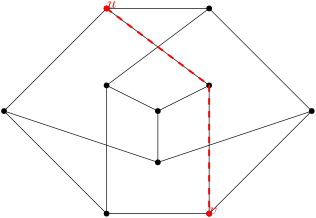
\includegraphics[width=0.5\linewidth]{img/grafi-razdalja.png}
        \caption{Razdalja med vozliščema}
    \end{figure}
\end{zgled}

{\definicija Premer} grafa je
\[
    \mathrm{diam}(G) = \max_{u,v \in G} d(u,v),
\]
se pravi največja možna razdalja med vsakim parom vozlišč. Premer je invarianta grafov.

\begin{domacanaloga}
    Prepričaj se, da je premer grafa iz zadnjega zgleda enak $2$. Določi še premer Petersenovega grafa.
\end{domacanaloga}

\section{Drevesa}

Grafu, ki ne vsebuje ciklov, pravimo {\definicija gozd}. Povezanemu gozdu pravimo {\definicija drevo}.

\begin{zgled}
Drevo je povezan graf brez ciklov. Njegova vozlišča stopnje $1$ so listi.
\begin{figure}[h]
    \centering
    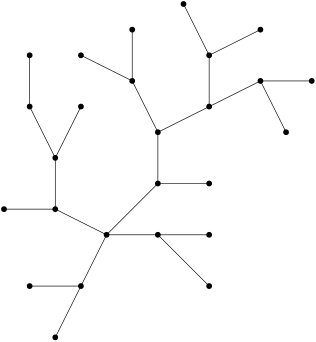
\includegraphics[width=0.5\linewidth]{img/grafi-drevo.png}
    \caption{Drevo}
\end{figure}    
\end{zgled}

Ker drevesa nimajo ciklov, so dvodelna. Imajo pa drevesa še veliko drugih čudovitih lastnosti.

\begin{trditev}
    Naj bo $T$ drevo.
    \begin{enumerate}
        \item Če je $|V(T)| > 1$, potem ima $T$ vsaj $2$ lista.
        \item $|E(T)| = |V(T)| - 1$.
        \item Za vsaka $u,v \in V(T)$ obstaja \emph{natanko ena} pot od $u$ do $v$.
    \end{enumerate}
\end{trditev}
\begin{dokaz}
1. Naj bo $P$ pot \emph{nadaljše možne dolžine} v drevesu $T$. Naj bo $u$ začetek in $v$ konec poti $P$. Trdimo, da je $d(u) = d(v) = 1$. Uporabimo dokaz s protislovjem. Naj bo $w$ predzadnje vozlišče na poti $P$. Predpostavimo, da velja $d(v) \geq 2$. Torej obstaja vozlišče $x \in V$, $x \neq w$, $x \sim v$. Ker v grafu $T$ ni ciklov, vozlišče $x$ ni na poti $P$. Zato lahko pot $P$ podaljšamo s povezavo $v \sim x$. To je protislovje z izbiro najdaljše možne poti $P$. Torej je res $d(v) = 1$. Podobno dokažemo $d(u) = 1$. Vozlišči $u$ in $v$ sta torej lista drevesa. \kljuka

2. Dokazujemo z indukcijo na $n = |V(T)|$. Baza je primer $n = 1$, ko drevo $T$ sestoji iz enega samega vozlišča in nima nič povezav. V tem primeru formula $0 = 1 - 1$ seveda drži. Za indukcijski korak predpostavimo, da formula drži za vsako drevo na $n$ vozliščih in naj bo $T$ drevo na $n+1$ vozliščih. Naj bo $v$ list $T$, ki obstaja po prejšnji točki. Naj bo $T' = T - v$. Tedaj je graf $T'$ brez ciklov in povezan,\footnote{List $v$ je lahko le začetek ali konec poti, zato pot med vozliščema $x,y \in V(T)$, $x,y \neq v$, \emph{ne} vsebuje $v$.} torej je $T'$ drevo z $n$ vozlišči. Po indukcijski predpostavki sledi $|E(T')| = n - 1$. Hkrati velja $|E(T)| = |E(T')| + 1$, torej ima drevo $T$ natanko $n$ povezav in formula velja. \kljuka

3. Predpostavimo, da obstajata različni poti od nekega vozlišča $u$ do nekega vozlišča $v$, recimo jima $P_1, P_2$. Naj bo $w$ zadnje vozlišče, v katerem se $P_1, P_2$ še ujemata. Naj bo $x$ prvo vozlišče na $P_1$ po $w$, ki je hkrati na $P_2$. Tedaj dobimo cikel $wP_1xP_2w$. To je protislovje, ker je $T$ drevo. \kljuka
\end{dokaz}

Drevesa zelo preprosto postanejo nepovezana. Povezava $e$ v povezanem grafu $G$ je {\definicija most}, če graf $G - e$ \emph{ni} povezan. Vsaka povezava, ki povezuje list s preostankom drevesa, je most. Res pa je še več.

\begin{trditev}
Vsaka povezava v drevesu je most.
\end{trditev}
\begin{dokaz}
    Naj bo $T$ drevo. Naj bo $e = \{ u, v \}$ poljubna povezava v $T$. Po zadnji trditvi je ta povezava \emph{edina} pot od $u$ do $v$ v drevesu $T$. Torej v grafu $T - e$ \emph{ne} obstaja pot od $u$ do $v$. To pomeni, da graf $T - e$ ni povezan. Povezava $e$ je torej most.
\end{dokaz}

Vse te čudovite lastnosti, ki jih imajo drevesa, v resnici \emph{karakterizirajo} drevesa.

\begin{trditev}
    Naj bo $G$ graf. Naslednje trditve so ekvivalentne.
    \begin{enumerate}
        \item $G$ je drevo.
        \item Med vsakima dvema vozliščema v $G$ obstaja natanko ena pot.
        \item $G$ je povezan in $|E(G)| = |V(G)| - 1$.
        \item $G$ je povezan in vsaka njegova povezava je most.
    \end{enumerate}
\end{trditev}
\begin{dokaz}
Po predzadnji trditvi vemo, da 1. $\Rightarrow$ 2. in 1. $\Rightarrow$ 3. Po zadnji trditvi vemo, da celo 2. $\Rightarrow$ 4.\footnote{V dokazu trditve smo namreč uporabili le lastnost 2. drevesa.} Dokažimo zdaj še 4. $\Rightarrow$ 1. in 3. $\Rightarrow$ 1.

4. $\Rightarrow$ 1.: Predpostavimo, da $G$ ni drevo in da v $G$ torej obstaja cikel $C$. Naj bo $e$ povezava na $C$. Tedaj po predpostavki graf $G - e$ \emph{ni} povezan. Naj bosta $x,y$ vozlišči grafa $G$, ki nista povezani v $G - e$. Ker je graf $G$ povezan, obstaja pot $P$ od $x$ do $y$ v $G$. Ta pot nujno prečka povezavo $e$. Nadomestimo to prečkanje povezave $e$ s potjo $C - e$. Torej v grafu $G - e$ obstaja sprehod od $x$ do $y$, zato pa tudi pot. To je protislovje z izbiro vozlišč $x,y$. Torej cikel $C$ v $G$ ne obstaja in $G$ je res drevo. \kljuka

3. $\Rightarrow$ 1.: Predpostavimo, da $G$ ni drevo in da v $G$ torej obstaja cikel $C$. Za vsako vozlišče $v \in V(G) \backslash V(C)$ izberimo pot $P_v$ najkrajše možne dolžine od $v$ do cikla $C$. Naj bo $e_v$ prva povezava na poti $P_v$. Trdimo, da za $u \neq v$ velja $e_u \neq e_v$. Res, če je $e_u = e_v$, potem sta $u$ in $v$ nujno povezani vozlišči vozlišče $u$ je povezano s ciklom $C$ s potjo $P_v - e$. Torej je dolžina poti $P_u$, ki je najkrajše možne dolžine, enaka kvečjemu dolžini poti $P_v$ manj $1$. Od tod sledi, da je dolžina poti $P_u - e$ strogo manjša od dolžine poti $P_v$. Torej smo našli pot, ki povezuje $u$ s $C$ in je krajše dolžine kot $P_v$. To je protislovje. Res torej za $u \neq v$ velja $e_u \neq e_v$. Od tod sledi
\[
    |E(G)| \geq |E(C)| + |\{ e_v \mid v \in V(G) \backslash V(C) \}|
    = |V(C)| + (|V(G)| - |V(C)|)
    = |V(G)|.
\]
Dobljeno je sprto s predpostavko $|E(G)| = |V(G)| - 1$. Cikel $C$ v $G$ torej ne obstaja in $G$ je res drevo. \kljuka
\end{dokaz}


\section{Eulerjevi grafi}

Sprehod v grafu je {\definicija Eulerjev sprehod}, če vsebuje \emph{vsako povezavo} grafa natanko enkrat. {\definicija Eulerjev obhod} je obhod, ki je Eulerjev sprehod.

\begin{zgled}
Lizika vsebuje Eulerjev sprehod, cikel $C_5$ vsebuje Eulerjev obhod, poln graf $K_5$ vsebuje Eulerjev obhod.
\end{zgled}

Graf je {\definicija Eulerjev}, če vsebuje Eulerjev obhod. Za to, da je graf Eulerjev, morata biti izpolnjena naslednja dva pogoja:
\begin{itemize}
    \item graf je povezan,
    \item vsa vozlišča so sode stopnje.\footnote{Če namreč med Eulerjevim obhodom pridemo v neko vozlišče, moramo iz njega tudi oditi. Enako velja za začetno vozlišče obhoda, ki je enako končnemu.}
\end{itemize}

Presenetljivo pa sta ta dva očitna potrebna pogoja tudi zadostna.

\begin{izrek}
    Naj bo $G$ povezan graf. Potem je $G$ Eulerjev natanko tedaj, ko so vsa vozlišča sode stopnje.
\end{izrek}
\begin{dokaz}
Dokazujemo le implikacijo iz desne v levo. Naj bo $S$ sprehod najdaljše možne dolžine v $G$, ki vsebuje vsako povezavo v $G$ \emph{kvečjemu enkrat}. Naj bo $u$ začetno vozlišče $S$ in $v$ končno vozlišče. Za vsakega soseda $w \sim u$ mora biti tudi povezava $\{ u, w \}$ na $S$, sicer lahko $S$ podaljšamo. Ker je $u$ sode stopnje in se sprehod $S$ začne v $u$, se mora tudi končati v $u$.\footnote{Vsaka povezava, ki je na $S$ in vstopi v $u$ in ni začetna povezava na $S$, mora iz $u$ tudi izstopiti.} Torej je $u = v$ in sprehod $S$ je v resnici \emph{obhod}. 

Premislimo, da je ta obhod Eulerjev. Res, če ni, potem izberimo neko povezavo $e = \{ x, y \}$, ki ni na $S$. Naj bo $Q$ neka najkrajša pot od $y$ do sprehoda $S$.\footnote{Taka pot obstaja, ker je graf $G$ povezan.}, zapišimo $Q = y \cdots z$ za vozlišče $z$ na obhodu $S$. Ker je $Q$ najkrajša, nobeno od njegovih vozlišč razen $v$ ne leži na $S$. Potemtakem je sprehod $xy \cdots v \cdots y \cdots v$, kjer se najprej sprehodimo od $x$ do $y$ prek $e$, potem od $y$ do $v$ prek $Q$ in nazadnje od $v$ do $v$ prek $S$, daljši od $S$ in vsako povezavo vsebuje kvečjemu enkrat. To je protislovje z izbiro $S$.
\end{dokaz}

Soroden kriterij imamo na voljo tudi za Eulerjeve sprehode.

\begin{izrek}
Naj bo $G$ povezan graf. Potem ima $G$ Eulerjev sprehod natanko tedaj, ko ima največ $2$ vozlišči lihe stopnje.
\end{izrek}
\begin{dokaz}
$(\Rightarrow)$: Vsa vozlišča razen morda začetnega in končnega imajo sodo stopnjo, ker za vsako vhodno povezavo obstaja izhodna. \kljuka

$(\Leftarrow)$: Število vozlišč lihe stopnje je sodo po lemi o rokovanju, torej je lahko enako le $0$ ali $2$. 
\begin{itemize}
    \item Če je enako $0$, potem so vsa vozlišča sode stopnje, zato obstaja celo Eulerjev obhod. \kljuka
    \item Če je enako $2$, potem vozlišči lihe stopnje označimo z $u,v$. Dodajmo povezavo $\{ u, v \}$ grafu $G$. Nov graf $G + uv$ ima vsa vozlišča sode stopnje, torej ima Eulerjev obhod $S$. Tedaj je $S - uv$ Eulerjev sprehod v grafu $G$. \kljuka
\end{itemize}
\end{dokaz}

\subsection{Mostovi}

Eulerjeva izvirna motivacija za študiranje obhodov v grafih, ki jim danes pravimo Eulerjevi obhodi, je bil {\definicija problem königsberških mostov}. Ta vprašuje, ali se je v takratnem mestu Königsberg\footnote{Danes imenovanem Kaliningrad.} bilo mogoče sprehoditi po mestu na tak način, da bi začeli in končali sprehod na isti točki, pri tem pa bi se po vsakem od mostov mesta sprehodili natanko enkrat.\footnote{Ta problem je Euler razrešil leta 1736.}

\begin{figure}[h]
    \centering
    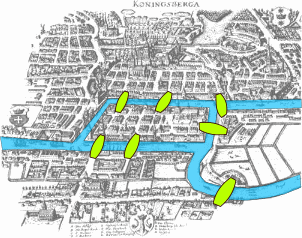
\includegraphics[width=0.5\linewidth]{img/konigsberg.png}
    \caption{Mostovi v Königsbergu, vir: Wikipedia}
\end{figure}    

Ta problem lahko prevedemo na teorijo grafo na naslednji način. Vsaki zemeljski masi priredimo vozlišče, mostu pa povezavo. Dobimo multigraf s štirimi vozlišči, eno je stopnje $5$, tri pa so stopnje $3$. Po dokazanih izrekih\footnote{Ni se težko prepričati, da ta dva izreka veljata tudi za multigrafe.} o obstoju Eulerjeve poti oziroma obhoda sklepamo, da v tem grafu ne obstaja niti Eulerjev sprehod. Želen obhod v mestu torej ni mogoč. 

\begin{figure}[h]
    \centering
    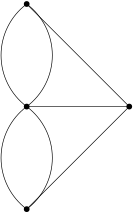
\includegraphics[width=0.25\linewidth]{img/grafi-konigsberg.png}
    \caption{Graf königsberških mostov}
\end{figure}    

Sorodno lahko obravnavamo {\definicija problem ljubljanskih mostov}. Ljubljana ima sicer bistveno več mostov kot stari Königsberg, zato se osredotočimo le na centralni del mesta, ki ga severno od gradu omejuje Ljubljanica, južno pa Gruberjev prekop.

\begin{figure}[h]
    \centering
    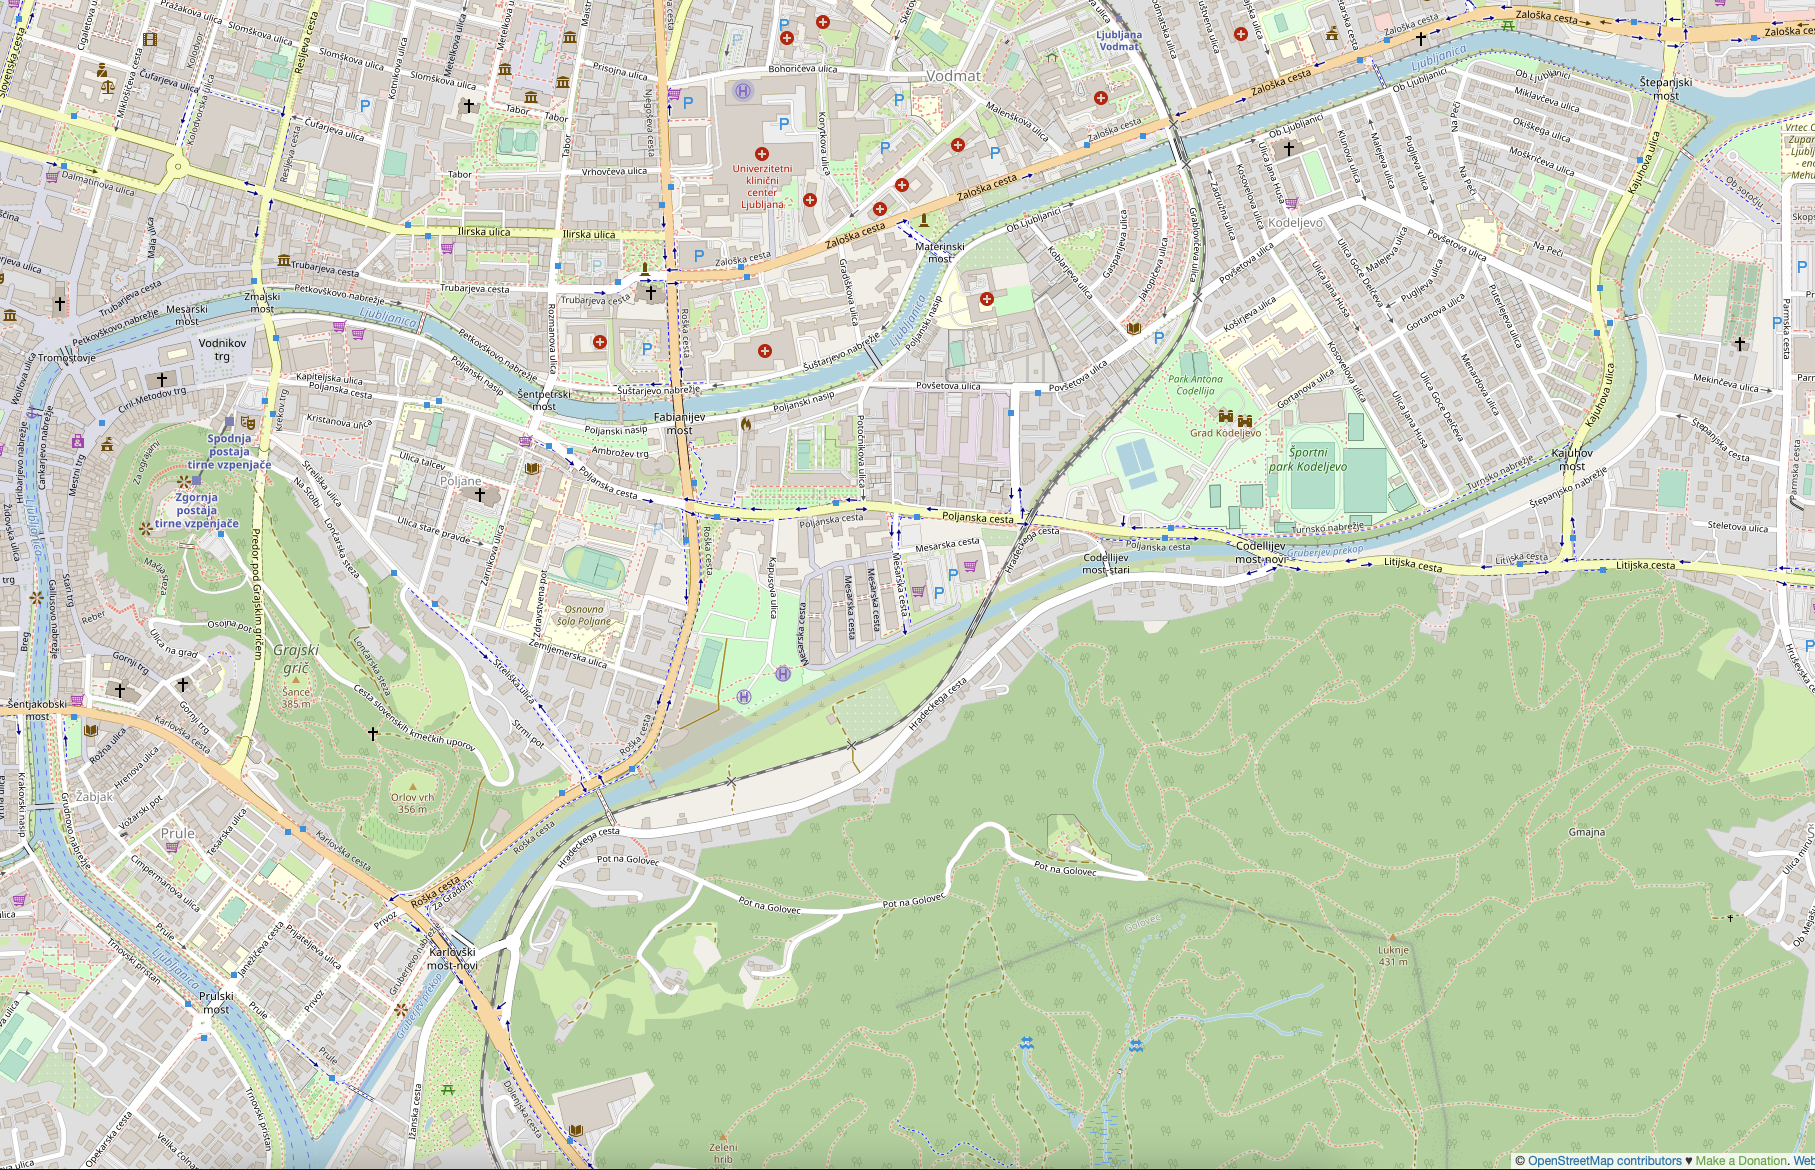
\includegraphics[width=1\linewidth]{img/ljubljana.png}
    \caption{Ljubljanski mostovi, vir: OpenStreetMap}
\end{figure}    

Imamo torej tri zemeljske mase: severo-zahodno (vključuje FMF), osrednjo (vključuje grad) in južno (vključuje Golovec). Prva je z drugo povezana z $18$ mostovi, druga pa s tretjo z $9$ mostovi. Dobimo torej multigraf s tremi vozlišči stopnje $18$, $27$ in $9$. Po izreku v centralni Ljubljani Eulerjev obhod ne obstaja, obstaja pa Eulerjev sprehod. Pri tem moramo v slednjem začeti in končati sprehod v vozliščih lihe stopnje, torej v posebnem ne na FMF.

\subsection{Risanje grafa v eni potezi}

Dan je graf. Ali ga lahko narišemo v eni potezi? Se pravi, ali lahko na list papirja narišemo graf tako, da vzamemo v roke pisalo, se z njim dotaknemo papirja, neprekinjeno rišemo povezave grafa (brez da bi večkrat potegnili pisalo čez isto povezavo) in na ta način narišemo vse povezave grafa? 

Ta problem je enakovreden temu, da v grafu najdemo Eulerjev sprehod, ki ga lahko neprekinjeno narišemo. Če graf nima Eulerjevega sprehoda, ga torej v eni potezi ne moremo narisati.

\begin{zgled}
Oglejmo si naslednji graf.

\begin{figure}[h]
    \centering
    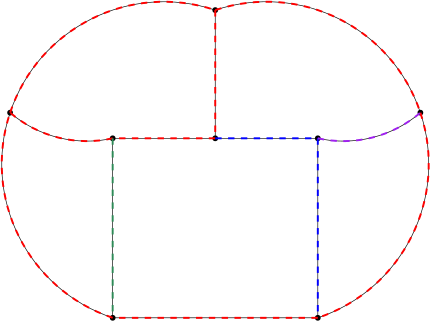
\includegraphics[width=0.5\linewidth]{img/grafi-enapoteza.png}
    \caption{Risanje grafa s čim manj potezami}
\end{figure}    

Ta graf je kubičen, zato nima Eulerjevega obhoda in ga ne moremo narisati v eni potezi. Kolikšno je najmanjše število potez, ki zadoščajo, da narišemo ta graf? Na sliki je prikazano, kako ta graf lahko narišemo s $4$ potezami. Vsaka poteza je prikazana s svojo barvo. Prepričajmo se, da pa tega grafa ne moremo narisati z manj kot $4$ potezami. To lahko vidimo tako, da seštejemo stopnje vseh vozlišč v grafu. Po lemi o rokovanju je ta vsota soda. Po drugi strani ima vsaka poteza svoje začetno in končno vozlišče (morda sta to enaki vozlišči), torej skupno prispeva k vsoti stopenj $2$ za vozlišča na sprehodu in $1$ za začetno in končno vozlišče. Graf, narisan v $3$ potezah, bi zato imel kvečjemu $6$ vozlišč lihe stopnje. Obravnavan graf pa ima $8$ vozlišč stopnje $3$.
\end{zgled}

Zadnji zgled lahko posplošimo na naslednji način.

\begin{trditev}
Naj bo $G$ povezan graf z $\ell$ vozlišči lihe stopnje. Najmanjše število potez, s katerimi lahko narišemo $G$, je $1$ za $\ell = 0$ in $\ell/2$ za $\ell > 0$.
\end{trditev}
\begin{dokaz}
Po lemi o rokovanju je $\ell$ sodo število. Če je $\ell = 0$, po izreku obstaja Eulerjev obhod, torej lahko graf narišemo v eni potezi. Če pa je $\ell > 0$, potem po argumentu v zadnjem zgledu gotovo potrebujemo vsaj $\ell/2$ potez, da narišemo graf $G$. Prepričajmo se, da $\ell/2$ potez tudi zadostuje. Res, naj bodo $u_1, u_2, \dots, u_{\ell/2}$ ter $v_1, v_2, \dots, v_{\ell/2}$ vozlišča lihe stopnje v $G$. Tedaj graf $G + u_1 v_1 + u_2 v_2 + \cdots u_{\ell/2} v_{\ell/2}$ nima vozlišč lihe stopnje, torej ima Eulerjev obhod
\[
    S = u_1 v_1 \cdots u_2 v_2 \cdots u_{\ell/2} v_{\ell/2} \cdots u_1.
\]
To pomeni, da lahko graf $G$ narišemo v $\ell/2$ potezah, in sicer v 1. potezi narišemo del $S$ od $v_1$ do $u_2$, v 2. potezi narišemo del $S$ od $u_2$ do $v_2$, \dots, v $\ell/2$-ti potezi narišemo del $S$ od $v_{\ell/2}$ do $u_1$.
\end{dokaz}

\section{Hamiltonovi grafi}

Hamiltonovi grafi so analogni Eulerjevim, kjer le zamenjamo vlogo povezav in vozlišč. Vpeta pot v grafu je {\definicija Hamiltonova pot}. Vpeti cikel v grafu je {\definicija Hamiltonov cikel}. 

\begin{zgled}
    \leavevmode
    \begin{itemize}
        \item Lizika vsebuje Hamiltonovo pot, poln graf $K_4$ vsebuje Hamiltonov cikel.
        \item Naslednji grafi vsebujejo Hamiltonove cikle, ki so označeni z rdečo barvo.
        
        \begin{figure}[h]
            \centering
            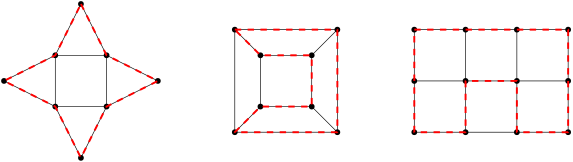
\includegraphics[width=1\linewidth]{img/grafi-hamilton.png}
            \caption{Grafi s Hamiltonovim ciklom}
        \end{figure}  

        \item Ali naslednji graf vsebuje Hamiltonov cikel?

        \begin{figure}[h]
            \centering
            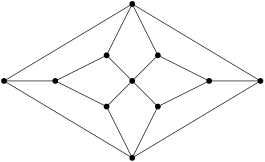
\includegraphics[width=0.5\linewidth]{img/grafi-hamilton-zgled.png}
            \caption{Ali ta graf vsebuje Hamiltonov cikel?}
        \end{figure}  

    \end{itemize}
\end{zgled}

Graf je {\definicija Hamiltonov}, če vsebuje Hamiltonov cikel. 

V prejšnjem razdelku smo spoznali, da lahko za poljuben graf zelo hitro ugotovimo, ali je Eulerjev. Za ugotavljanje hamiltonskosti grafa pa ni znan noben preprost postopek, ki bi bil uporaben za vse grafe. Preverjanje hamiltonskosti je običajno bistveno težji problem od preverjanja, ali je graf Eulerjev.\footnote{Hamilton je Hamiltonove grafe opazoval približno sto let po Eulerju.} Poznanih pa je nekaj \emph{potrebnih} pogojev in nekaj \emph{zadostnih} pogojev za hamiltonskost. 

\begin{izrek}[potreben pogoj za hamiltonskost]
Naj bo $G$ graf. Predpostavimo, da v $G$ obstaja neprazna podmnožica $S \subseteq V(G)$, za katero velja $\Omega(G-S) > |S|$. Tedaj graf $G$ \emph{ni} Hamiltonov.
\end{izrek}
\begin{dokaz}
Predpostavimo, da je $G$ Hamiltonov graf s Hamiltonovim ciklom $C$. Naj bo $S$ neka neprazna množica vozlišč grafa $G$. Ko odstranimo vozlišča $S$ s cikla $C$, ta cikel razpade na kvečjemu $|S|$ komponent (krožnih lokov). Ti loki so prek povezav grafa $G$, ki ne ležijo na ciklu $C$, lahko morda še povezani med sabo. Graf $G - S$ ima zatorej kvečjemu $|S|$ komponent in velja torej $\Omega(G - S) \leq |S|$. S tem je dokaz zaključen.
\end{dokaz}

\begin{zgled}
Ko liziki odstranimo vozlišče stopnje $3$, razpade na dve komponenti. Lizika torej ni Hamiltonov graf.
\end{zgled}

Zabeležimo poseben primer dokazanega izreka za dvodelne grafe.

\begin{posledica}
Naj bo $G$ dvodelen graf z $V(G) = A \cup B$, $A \cap B = \emptyset$, pri čemer ima vsaka povezava v $E(G)$ eno krajišče v $A$, drugo pa v $B$. Če je $|A| \neq |B|$, potem $G$ \emph{ni} Hamiltonov.
\end{posledica}
\begin{dokaz}
    Brez škode za splošnost lahko predpostavimo, da velja $|A| < |B|$. Vzemimo $S = A$. Ko v grafu $G$ odstranimo vozlišča $A$, nam ostane graf z vozlišči $B$ in brez povezav. Velja torej $\Omega(G-A) = |B| > |A|$. Po izreku graf $G$ zato ni Hamiltonov.
\end{dokaz}

\begin{zgled}
Vrnimo se k zadnjemu zgledu iz začetka tega razdelka. Obravnavani graf je dvodelen z biparticijo vozlišč $A \cup B$, pri čemer je $|A| = 5$ in $|B| = 6$. Po posledici ta graf zato ni Hamiltonov.

\begin{figure}[h]
    \centering
    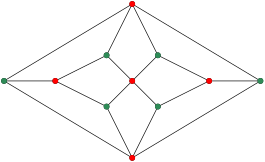
\includegraphics[width=0.5\linewidth]{img/grafi-hamilton-zgled-dvodelen.png}
    \caption{Dvodelen graf, ki ni Hamiltonov}
\end{figure}  
\end{zgled}

Analogen potreben pogoj lahko izpeljemo za obstoj Hamiltonove poti.

\begin{izrek}[potreben pogoj za obstoj Hamiltonove poti]
Naj bo $G$ graf. Predpostavimo, da v $G$ obstaja neprazna podmnožica $S \subseteq V(G)$, za katero velja $\Omega(G-S) > |S| + 1$. Tedaj graf $G$ \emph{nima} Hamiltonove poti.   
\end{izrek}
\begin{dokaz}
    Predpostavimo, da ima $G$ Hamiltonovo pot $P$. Naj bo $S$ neka neprazna množica vozlišč grafa $G$. Ko odstranimo vozlišča $S$ s poti $P$, ta pot razpade na kvečjemu $|S|+1$ komponent (delov poti). Ti deli so prek povezav grafa $G$, ki ne ležijo na poti $P$, lahko morda še povezani med sabo. Graf $G - S$ ima zatorej kvečjemu $|S| + 1$ komponent in velja torej $\Omega(G - S) \leq |S| + 1$. S tem je dokaz zaključen.
\end{dokaz}

\begin{zgled}
Dvodelen graf iz zadnjega zgleda ni Hamiltonov, saj z odstranitvijo $5$ točk graf razpade na $6$ komponent. Iz tega argumenta pa še ne sledi, da ta graf nima Hamiltonove poti, saj bi za to moral razpasti na vsaj $7$ komponent. V resnici ta graf ima Hamiltonovo pot, kot je prikazano na naslednji sliki. 

\begin{figure}[h]
    \centering
    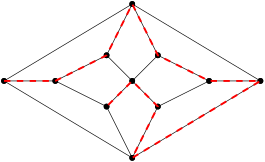
\includegraphics[width=0.5\linewidth]{img/grafi-hamilton-zgled-pot.png}
    \caption{Hamiltonova pot v grafu}
\end{figure}  
\end{zgled}

Zdaj si bomo pogledali še nekaj zadostnih pogojev za hamiltonskost. Naslonili jih bomo na naslednjo lemo.

\begin{lema}
    Naj za vozlišči $u,v$ grafa $G$ velja $u \neq v$, $u \not\sim v$, $d(u) + d(v) \geq |V(G)|$. Tedaj je $G$ Hamiltonov, če in samo če je $G + uv$ Hamiltonov.
\end{lema}
\begin{dokaz}
$(\Rightarrow)$: Če je graf $G$ Hamiltonov s Hamiltonovim ciklom $C$, potem je isti cikel $C$ tudi Hamiltonov cikel v grafu $G + uv$. \kljuka

$(\Leftarrow)$: Naj bo $C$ Hamiltonov cikel v grafu $G + uv$. Privzemimo, da $G$ ni Hamiltonov graf. Torej je povezava $uv$ nujno na ciklu $C$. Graf $G$ zato vsebuje Hamiltonovo pot $C - uv = v_1 v_2 \dots v_n$ z začetkom v $u = v_1$ in koncem v $v = v_n$, pri čemer je $n = |V(G)|$.

Opazumo sosede vozlišča $u$. Recimo, da za nek $i < n$ velja $u \sim v_{i+1}$. Premislimo, da tedaj vozlišče $v$ ni povezano z neposrednim predhodnikom vozlišča $v_{i+1}$, to je $v_i$. Res, če je $v \sim v_i$, potem v $G$ najdemo Hamiltonov cikel $v_1 \dots v_i v_n \dots v_{i+1} v_1$, ki pa po predpostavki ne obstaja.

Noben od $d(u)$ neposrednih predhodnikov sosedov $u$ torej ni sosed $v$. To pomeni, da je število sosedov $v$ enako kvečjemu $n - 1 - d(u)$, kjer smo upoštevali še, da vozlišče $v$ ni povezano samo s sabo. Od tod sledi $d(v) \leq n - 1 - d(u)$, kar je enakovredno $d(u) + d(v) \leq n -1$. To je sprto s predpostavko $d(u) + d(v) \geq n = |V(G)|$. Graf $G$ je nazadnje torej res Hamiltonov. \kljuka
\end{dokaz}

\begin{izrek}[Ore]
    Naj bo $G$ graf z $|V(G)| \geq 3$. Če za vsaki dve vozlišči $u,v \in V(G)$ z lastnostjo $u \neq v$, $u \not\sim v$ velja $d(u) + d(v) \geq |V(G)|$, potem je $G$ Hamiltonov.
\end{izrek}
\begin{dokaz}
Grafu $G$ dodajamo povezave, dokler ne dobimo polnega grafa $K_n$. Po lemi je graf $G$ Hamiltonov, če in samo če je $K_n$ Hamiltonov, kar pa je res (za $\geq 3$).
\end{dokaz}

\begin{zgled}
    Za vsaki različni nepovezani vozlišči v naslednjem grafu velja $d(u) + d(v) \geq 7$. Po Orejevem izreku je graf Hamiltonov. Poišči Hamiltonov cikel v njem!

    \begin{figure}[h]
        \centering
        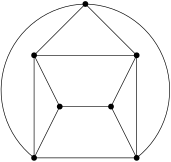
\includegraphics[width=0.5\linewidth]{img/grafi-hamilton-ore.png}
        \caption{Hamiltonov graf po Orejevem izreku}
    \end{figure}  
\end{zgled}

\begin{izrek}[Dirac]
    Naj bo $G$ graf z $|V(G)| \geq 3$. Če je $\delta(G) \geq |V(G)|/2$, potem je $G$ Hamiltonov.
\end{izrek}
\begin{dokaz}
    Po predpostavki za vsaki vozlišči $u,v \in V(G)$ velja $d(u) + d(v) \geq |V(G)|$. Po Orejevem izreku je graf $G$ zato Hamiltonov.
\end{dokaz}

\begin{zgled}
    Najmanjša stopnja vozlišča v naslednjem grafu je $3$, število vozlišč pa je $6$. Po Diracovem izreku je graf Hamiltonov. Poišči Hamiltonov cikel v njem!

    \begin{figure}[h]
        \centering
        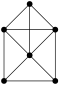
\includegraphics[width=0.25\linewidth]{img/grafi-hamilton-dirac.png}
        \caption{Hamiltonov graf po Diracovem izreku}
    \end{figure}  
\end{zgled}

Včasih se znajdemo v situaciji, ko nam ob danem grafu niti potrebni niti zadostni pogoji ne odgovorijo na vprašanje, ali je graf Hamiltonov. V tem primeru posežemo po bolj ad hoc tehnikah, kot je prikazano v naslednjem zgledu.

\begin{zgled}
    Ali je Petersenov graf Hamiltonov? Na naslednji sliki je prikazana Hamiltonova pot.

    \begin{figure}[h]
        \centering
        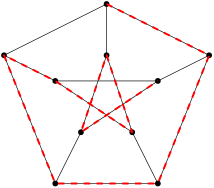
\includegraphics[width=0.25\linewidth]{img/grafi-petersen-hamilton-pot.png}
        \caption{Hamiltonova pot v Petersenovem grafu}
    \end{figure}     

    S protislovjem premislimo, da Hamiltonov cikel ne obstaja. Če bi namreč $C$ bil Hamiltonov cikel, potem bi vseboval $10$ vozlišč Petersenovega grafa in $10$ povezav. Označimo vozlišča na $C$ z $v_1v_2 \dots v_{10}$. Ker ima Petersenov graf $15$ povezav, iščemo torej še $5$ dodatnih tetivnih povezav, ki jih dodamo ciklu $C$, da dobimo Petersenov graf. Vemo, da je Petersenov graf $3$-regularen, zato moramo po eno tako tetivno povezavo dodati vsakemu vozlišči na ciklu $C$. Vemo, da Petersenov graf nima $3$-ciklov in nima $4$-ciklov, hkrati pa ima $5$-cikel. Gotovo torej obstaja vozlišče na $C$, brez škode je to kar $v_1$, ki ima tetivno povezavo do soseda antipodnega vozlišča $v_6$, brez škode je to kar $v_5$. Opazujmo zdaj vozlišče $v_6$. Tudi to vozlišče mora imeti tetivno povezavo do nekega vozlišča na $C$. Ker pa Petersenov graf nima $3$-ciklov in nima $4$-ciklov, taka tetivna povezava ne obstaja. To je protislovje z obstojem Hamiltonovega cikla v Petersenovem grafu.
\end{zgled}

\subsection{Šahovski konjiček}

Opazujmo gibanje šahovskega konjička na šahovnici dimenzij $m \times n$. Ali lahko konjiček z zaporedjem skokov obišče vsako polje šahovnice natanko enkrat in zaključi na začetnem polju? To je problem {\definicija požrešnega šahovskega konjička}. 

Polja šahovnice si lahko predstavljamo kot vozlišča grafa, možnost skoka konjička iz enega polja na drugega pa predstavimo s povezavo. V tem smislu je problem požrešnega šahovskega konjička enakovreden obstoju Hamiltonovega cikla v tem grafu.

\begin{figure}[h]
    \centering
    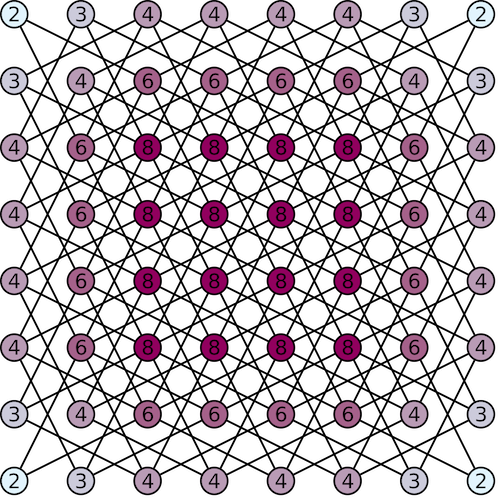
\includegraphics[width=0.5\linewidth]{img/grafi-konjicek-graf.png}
    \caption{Graf, ki prikazuje možne skoke konjička na šahovski plošči $8 \times 8$; v vozliščih so vpisane stopnje, vir: Wikipedia}
\end{figure}    

Poglejmo si nekaj posebnih primerov.

\begin{zgled} \leavevmode
\begin{itemize}
    \item Obravnavajmo šahovnico dimenzij $3 \times 3$. Če konjiček začne v centralnem polju, potem nima kam skočiti, saj je plošča premajhna. Centralno vozlišče prirejenega grafa je torej izolirana točka in graf ni povezan, zato seveda tudi nima Hamiltonovega cikla.
    \item Obravnavajmo šahovnico dimenzij $5 \times 5$. Dobimo graf na $25$ vozliščih. Če obarvamo vozlišča s črno in belo barvo kot na šahovnici, potem je zaradi dejstva, da konjiček vedno skoči s črnega polja na belo oziroma obratno, prirejeni graf \emph{dvodelen}. Ker ima šahovnica $25$ vozlišč, je število belih vozlišč različno od števila črnih vozlišč. Po izreku ta graf torej ni Hamiltonov. Enak argument deluje za vse šahovnice z lihim številom polj.
\end{itemize}
\end{zgled}

\begin{domacanaloga}
    Obravnavaj šahovnico dimenzije $4 \times n$ za $n \geq 4$. Dokaži, da Hamiltonov cikel \emph{ne} obstaja.\footnote{V pomoč ti bo, če vozlišča v vrsticah $1$ in $4$ obarvaš rdeče, vozlišča v vrsticah $2$ in $3$ pa modro. Konjiček lahko sicer skoči iz modrega vozlišča nazaj v modro vozlišče, na primer iz polja $(2,1)$ v $(3,3)$, ampak iz rdečega vozlišča pa konjiček lahko skoči le v modro vozlišče.}
\end{domacanaloga}

Izkaže se, da sta po eni strani lihost števila polj in po drugi strani premajhno število vrstic oziroma stolpcev šahovnice \emph{edini} oviri za obstoj Hamiltonovega cikla, a tega ne bomo dokazali.

\begin{izrek}[Schwenk]
    Konjičkov obhod na šahovnici $m \times n$ obstaja, če je le $m \cdot n$ sodo število in $m, n > 4$.
\end{izrek}

V posebnem torej obstaja obhod na standardni šahovnici $8 \times 8$.

\begin{figure}[h]
    \centering
    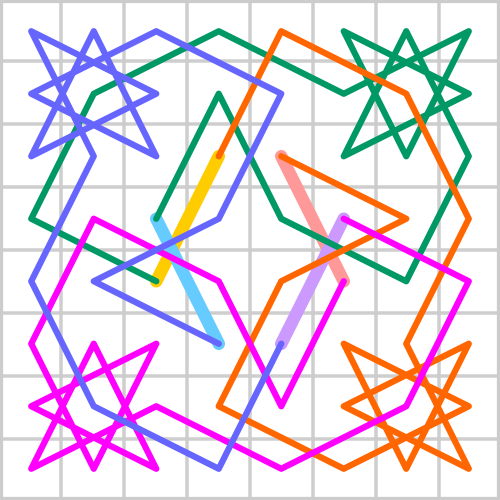
\includegraphics[width=0.5\linewidth]{img/grafi-konjicek.png}
    \caption{Konjičkov obhod na šahovnici $8 \times 8$, vir: Wikipedia}
\end{figure}  

\section{Ravninski grafi}

Obravnavajmo naslednji izziv, ki je na prvi pogled osnovnošolska naloga. Pred nami so $3$ hiše in $3$ drevesa. S potjo je potrebno povezati vsako hišo z vsakim drevesom, ne da bi se pri tem poti sekale med sabo. Če si vsako hišo oziroma drevo predstavljamo kot vozlišče, pot pa kot povezavo, potem pravzaprav vprašujemo, če lahko graf $K_{3,3}$ narišemo v ravnino tako, da se nobeni dve povezavi med sabo ne sekata (razen v vozliščih). Splošneje se lahko torej vprašamo, ali lahko poljuben graf narišemo v ravnini brez križanja povezav.

\begin{zgled}
    Nekatere grafe gotovo lahko narišemo v ravnini brez križanja povezav, na primer liziko, cikle, drevesa. Tudi poln graf $K_4$ lahko narišemo na ta način, kot je prikazano na sliki.

    \begin{figure}[h]
        \centering
        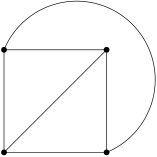
\includegraphics[width=0.5\linewidth]{img/grafi-ravninski-k4.png}
        \caption{Ravninski graf $K_4$}
    \end{figure}    
\end{zgled}

Po nekaj poskusih se zdi, da grafa $K_{3,3}$ ne moremo narisati na želeni način v ravnini. Kako bi dokazali, da je to res nemogoče? Preden lahko odgovorimo na to vprašanje, moramo najprej matematično bolj natančno formulirati problem.

{\definicija Vložitev grafa $G$ v ravnino} je injektivna preslikava $\phi \colon V(G) \to \RR^2$ skupaj z družino zveznih preslikav $\phi_e \colon [0,1] \to \RR^2$ za vsako povezavo $e \in E(G)$, da velja:
\begin{enumerate}
    \item če je $e = \{ u,v \} \in E(G)$, potem je $\{ \phi_e(0), \phi_e(1) \} = \{ \phi(u), \phi(v) \}$,\footnote{Preslikava $\phi_e$ torej preslika rob intervala $[0,1]$ v sliki krajišč povezave $e$ s povezavo $\phi$.}
    \item za vsak $e \in E(G)$ je $\phi_e|_{(0,1)}$ injektivna,\footnote{Pri risanju povezave $e$ ni nobenih samopresečnih točk.}
    \item za vsaka $e, e' \in E(G)$, $e \neq e'$, velja $\mathrm{im} \phi_e|_{(0,1)} \cap \mathrm{im} \phi_{e'}|_{(0,1)} = \emptyset$,\footnote{Tukaj smo z $\phi_e |_{(0,1)}$ označili zožitev preslikave $\phi_e$ na odprti interval $(0,1)$, z $\mathrm{im} f$ pa smo označili sliko preslikave $f$. Nobeni dve narisani povezavi se torej ne sekata (razen morda v robnih točkah).}
    \item za vsak $e \in E(G)$ velja $\mathrm{im} \phi_e|_{(0,1)} \cap \mathrm{im} \phi = \emptyset$.\footnote{Narisana povezava lahko prečka narisano vozlišče, če in samo če je to rob narisane povezave.}
\end{enumerate}
Vse podatke o vložitvi grafa v ravnino zberemo v par $(\phi, \{ \phi_e \}_{e \in E(G)})$, ki ga krajše označimo kot $\GG$.\footnote{Oznako $G$ torej uporabljamo za abstraktni graf, se pravi $G = (V,E)$, oznako $\GG$ pa uporabljamo za vložitev grafa $G$ v ravnino, se pravi $\GG = (\phi, \{ \phi_e \}_{e \in E})$.}
    
Graf $G$ je {\definicija ravninski}, če ima kakšno vložitev v ravnino. Pri tem seveda lahko obstajajo različne vložitve.

\begin{zgled}
Disjunktno unijo $K_3 \cup K_3$ lahko narišemo v ravnino na dva vsaj načina, in sicer lahko en trikotnik narišemo znotraj drugega ali pa dva trikotnika narišemo enega ob drugem.

\begin{figure}[h]
    \centering
    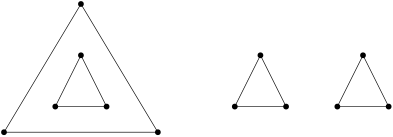
\includegraphics[width=0.5\linewidth]{img/grafi-ravninski-k3k3.png}
    \caption{Dve različni vložitvi grafa $K_3 \cup K_3$ v ravnino}
\end{figure} 
\end{zgled}

Vložitev grafa razdeli ravnino na povezane dele, ki jim pravimo {\definicija lica} vložitve. Vselej je natanko eno lice neomejeno -- imenujemo ga {\definicija zunanje lice}.

\begin{zgled} \leavevmode
    \begin{itemize}
        \item Vsaka ravninska vložitev drevesa ima eno samo lice, saj graf nima nobenih ciklov.
        \item Obe vložitvi grafa $K_3 \cup K_3$ iz zadnjega zgleda imata $3$ lica.

\begin{figure}[h]
    \centering
    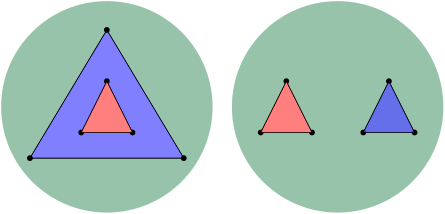
\includegraphics[width=0.5\linewidth]{img/grafi-ravninski-k3k3-lica.png}
    \caption{Lica vložitev grafa $K_3 \cup K_3$ v ravnino}
\end{figure} 
\end{itemize}
\end{zgled}


Naj bo $\GG$ vložitev grafa $G$ v ravnino. Označimo množico točk v ravnini, ki predstavljajo vozlišča, povezave in lica:
\begin{align*}
    V(\GG) &= \{ \phi(u) \mid u \in V(G) \} \subseteq \RR^2, \\
    E(\GG) &= \{ \mathrm{im} \phi_e \mid e \in E(G) \}, \\
    F(\GG) &= \{ f \mid \text{$f$ lice vložitve $\GG$}\}.
\end{align*}
{\definicija Dolžina lica} $f \in F(\GG)$ je število povezav, ki ležijo na robu lica $f$. To dolžino označimo z $\ell(f)$.

\begin{zgled}
Obravnavajmo ravninski vložitvi $K_3 \cup K_3$ iz zadnjega zgleda. V prvi ravninski vložitvi je dolžina rdečega lica enaka $3$, dolžina modrega je enaka $6$ in dolžina zelenega je enaka $3$. V drugi ravninski vložitvi sta dolžini modrega in rdečega lica enaki $3$, dolžina zelenega pa je enaka $6$.
\end{zgled}

\begin{izrek}[lema o rokovanju za ravninske grafe]
    Naj bo $G$ graf z ravninsko vložitvijo $\GG$. Potem je
    \[
        \sum_{f \in F(\GG)} \ell(f) = 2 \cdot |E(G)|.
    \]
\end{izrek}
\begin{dokaz}
Pristopimo podobno kot pri dokazu leme o rokovanju. Slika vsake povezave v $E(G)$ pripada robu dveh lic (vsakemu enkrat) ali enega samega lica (dvakrat). Naj bo $E(G) = \{ e_1, e_2, \dots, e_a \}$ in $F(\GG) = \{ f_1, f_2, \dots, f_b \}$. Definirajmo matriko $M = [m_{ij}]_{1 \leq i \leq a, 1 \leq j \leq b}$ razsežnosti $a \times b$ z vnosi
\[
    m_{ij} = \begin{cases}
        0 & \text{$e_j$ ni na robu $f_i$,} \\
        1 & \text{$e_j$ je na robu $f_i$ (enkrat),} \\
        2 & \text{$e_j$ je na robu $f_i$ (dvakrat).}
    \end{cases}
\]
Vsota vseh vnosov matrike $M$ je po eni strani enaka
\[
    \sum_{i = 1}^a \sum_{j = 1}^b m_{ij} = \sum_{i = 1}^a \ell(f_i) = \sum_{f \in F(\GG)} \ell(f),
\]
po drugi strani pa je enaka
\[
    \sum_{j = 1}^b \sum_{i = 1}^a  m_{ij} = \sum_{j = 1}^b 2 = 2b = 2 \cdot |E(G)|,
\]
s čimer je dokaz zaključen.
\end{dokaz}

Med števili $|V(\GG)|$, $|E(\GG)|$ in $|F(\GG)|$ velja naslednja povezava.

\begin{izrek}[Eulerjeva formula]
    Naj bo $G$ \emph{povezan} graf z ravninsko vložitvijo $\GG$. Tedaj je
    \[
        |V(\GG)| - |E(\GG)| + |F(\GG)| = 2.
    \]
\end{izrek}
\begin{dokaz}
Dokazujemo z indukcijo na število ciklov $c$ v grafu $G$.

Baza indukcije je $c = 0$. V tem primeru je $G$ drevo. Velja torej $|E(\GG)| = |V(\GG)| - 1$ in hkrati $|F(\GG)| = 1$, torej Eulerjeva formula velja. \kljuka

Privzemimo zdaj, da formula velja za vse grafe z največ $c$ cikli. Naj bo $G$ graf s $c+1$ cikli. Naj bo $C$ nek cikel v $G$ z povezavo $\{ u,v \}$ na $C$. Opazujmo graf $G' = G - uv$. Naj bo $\GG'$ ravninska vložitev tega grafa, ki ga dobimo iz ravninske vložitve $\GG$. Graf $G'$ je povezan in ima manj ciklov kot $G$, zato lahko na njem uporabimo indukcijsko predpostavko. Za ta graf velja $|V(G')| = |V(G)|$ in $|E(G')| = |E(G)| - 1$, hkrati pa se z odstranitvijo povezave $uv$ lici s skupnim robom $uv$ spojita v eno lice, zato je $|F(\GG')| = |F(\GG)| - 1$. Ker po indukcijski predpostavki velja $|V(\GG')| - |E(\GG')| + |F(\GG')| = 2$, od tod sledi $|V(\GG)| - |E(\GG)| + |F(\GG)| = 2$. \kljuka
\end{dokaz}

Eulerjevo formulo lahko posplošimo tudi na neravninske grafe.

\begin{posledica}
Naj bo $G$ graf z $\Omega$ povezanimi komponentami in z ravninsko vložitvijo $\GG$. Tedaj je
\[
    |V(\GG)| - |E(\GG)| + |F(\GG)| = 1 + \Omega.
\]
\end{posledica}
\begin{dokaz}
Naj bodo $G_1, G_2, \dots, G_\Omega$ povezane komponente grafa $G$. Dodajmo povezave $e_1, e_2, \dots, e_{\Omega - 1}$ grafu $G$, da postane povezan in da v vložitvi $\GG$ ne ustvarimo lic (na primer vse komponente grafa $G$ povežemo s prvo). Tedaj za graf $G + e_1 + e_2 + \cdots + e_{\Omega - 1}$ velja Eulerjeva formula. Ta graf ima enako število vozlišč in lic kot $\GG$, hkrati pa ima $\Omega-1$ več povezav. Velja torej
\[
    |V(\GG)| - (|E(\GG)| + \Omega - 1) + |F(\GG)| = 2,
\]
od koder sledi želeno
\[
    |V(\GG)| - |E(\GG)| + |F(\GG)| = 1 + \Omega.
\]
\end{dokaz}

S pomočjo Eulerjeve formule lahko izpeljemo \emph{potreben} pogoj za ravninskost grafa.

\begin{trditev}
    Naj bo $G$ ravninski graf z vsaj tremi vozlišči. Tedaj je
    \[
        |E(G)| \leq 3 \cdot |V(G)| - 6.
    \]
    Če je graf $G$ brez $3$-ciklov, potem je celo
    \[
        |E(G)| \leq 2 \cdot |V(G)| - 4.
    \]
\end{trditev}
\begin{dokaz}
    Naj bo $\GG$ ena od vložitev grafa $G$ v ravnino. Ocenimo število lic te vložitve. Vsako lice je dolžine vsaj $3$.\footnote{Ker ima $G$ vsaj $3$ vozlišča, je vsako lice omejeno s ciklom dolžine vsaj $3$ ali pa s $P_2$ (dvakrat).} Po lemi o rokovanju za ravninske grafe od tod sledi ocena
    \[
        2 \cdot |E(G)| = \sum_{f \in F(\GG)} \ell(f) \geq \sum_{f \in F(\GG)} 3 = 3 \cdot |F(\GG)|.
        \]
    Število lic lahko torej ocenimo navzgor kot $|F(\GG)| \leq \frac23 |E(G)|$. Iz Eulerjeve formule zdaj sledi
    \[
        2 \leq |V(G)| - |E(G)| + |F(\GG)| \leq |V(G)| - \frac13 |E(G)|,
    \]
    ker je enakovredno želeni neenakosti $|E(G)| \leq 3 \cdot |V(G)| - 6$.

    Če graf $G$ nima $3$-ciklov, potem je vsako lice dolžine vsaj $4$. Če torej v prvi neenakosti uporabimo to močnejšo oceno o dolžinah lic, z enakim postopkom dobimo še drugo neenakost v trditvi.
\end{dokaz}

\begin{zgled}
\leavevmode
\begin{itemize}
    \item Uporabimo zadnjo trditev za to, da dokažemo, da graf $K_{3,3}$, ki smo ga obravnavali na začetku tega razdelka, res ni ravninski. Ta graf ima $6$ vozlišč in $9$ povezav. Ker je dvodelen, ne vsebuje $3$-ciklov. Če bi bil ravninski, bi zanj torej morala veljati neenakost $9 \leq 2 \cdot 6 - 4 = 8$, kar pa ne drži.
    \item Premislimo, da tudi graf $K_5$ ni ravninski. Ta graf ima $5$ vozlišč in $10$ povezav. Če bi bil ravninski, bi zanj morala veljati neenakost $10 \leq 3 \cdot 5 - 6 = 9$, kar pa ne drži.
\end{itemize}
\end{zgled}

Naj bo $G$ ravninski graf. Če je $H$ \emph{podgraf} grafa $G$, potem je tudi $H$ ravninski, saj lahko iz ravninske vložitve $\GG$ preprosto odstranimo nepotrebna vozlišča in povezave. Na ta način lahko najdemo še več grafov, ki niso ravninski. Poznamo pa še dve malo bolj fleksibilni konstrukciji s podobno lastnostjo.

\begin{enumerate}
    \item Graf $H$ je {\definicija minor} grafa $G$, če ga lahko konstruiramo iz nekega podgrafa $G$ s \emph{krčenjem nekaterih povezav}.\footnote{Predstavljamo si, da izbrane povezave počasi krajšamo, dokler se krajišči ne združita. Po tem morebitne zanke odstranimo in vzporedne povezave identificiramo, da dobimo na koncu tega postopka res graf in ne multigrafa.}
    
    \begin{zgled}
        Če v Petersenovem grafu skrčimo povezave, ki povezujejo zunanji cikel z notranjim, dobimo graf $K_5$. Ta graf je torej minor Petersenovega grafa.
    \end{zgled}
        
    Minor ravninskega grafa je ravninski graf, saj lahko krčenje povezav v ravnini izvedemo tako, da pri tem ne pride do sekanja ostalih povezav.

    \begin{posledica}
        Če graf $G$ vsebuje minor $K_{3,3}$ ali $K_5$, potem ni ravninski.
    \end{posledica}

    \begin{zgled}
        Petersenov graf ni ravninski.
    \end{zgled}

    {\definicija Wagnerjev izrek} nam pove, da velja celo obrat posledice. Če graf $G$ \emph{ne} vsebuje minorja $K_{3,3}$ ali $K_5$, potem \emph{je} ravninski. Dokaz izpustimo.

    \item Graf $H$ je {\definicija subdivizija} grafa $G$, če ga lahko konstruiramo iz $G$ tako, da \emph{nekatere povezave nadomestimo s potmi dolžine $2$ ali več}.\footnote{Določenim povezavam torej dodamo nekaj vozlišč.}
        
    Subdivizija ravninskega grafa je ravninski graf.

    \begin{posledica}
        Če graf $G$ vsebuje subdivizijo $K_{3,3}$ ali $K_5$, potem ni ravninski.
    \end{posledica}

    {\definicija Izrek Kuratowskega} nam pove, da velja celo obrat posledice. Če graf $G$ \emph{ne} vsebuje subdivizije $K_{3,3}$ ali $K_5$, potem \emph{je} ravninski. Dokaz izpustimo.

    \begin{domacanaloga}
        Vemo že, da Petersenov graf ni ravninski. Po izreku Kuratowskega torej vsebuje subdivizijo $K_{3,3}$ ali $K_5$. Poišči to subdivizijo!
    \end{domacanaloga}
\end{enumerate}


\end{document}
